\NeedsTeXFormat{LaTeX2e}
\documentclass[12pt,a4paper,oneside,openright]{Book}
%\pagestyle{empty}
\usepackage[utf8]{vietnam}
\usepackage{listings}
\usepackage{indentfirst}
\usepackage{amsmath,amsfonts,amssymb,fancyhdr}
\usepackage{amsthm,amsxtra,latexsym, amscd}
\usepackage[top=3.5cm, bottom=3cm, left=3.5cm, right=2.0cm] {geometry}
\usepackage[unicode]{hyperref}
\usepackage{graphicx}
\graphicspath{images}
\usepackage{titlesec}
\usepackage{color}
\usepackage[table]{xcolor}
\graphicspath{ {images}}
\setcounter{secnumdepth}{5}
\usepackage{afterpage}
\usepackage{boxedminipage,fancybox}
%\hoffset=-0.3truecm %
%\voffset=-2.5truecm %
%\textheight=26truecm %
%\textwidth=16truecm %
%\oddsidemargin 28pt \footskip 30pt
\font\tench=t5-lmb10 at18pt%
\titleformat{\chapter}[display]
{\normalfont\large\filcenter\bfseries}
{{{\chaptertitlename\,}\thechapter}} {1pc}{%\vspace{1pc}%
{\tench}\MakeUppercase}% Dinh nghia lai ten chuong
%{\tench}}%\MakeUppercase}% Dinh nghia lai ten chuong

\renewcommand{\theequation}{\thechapter.\arabic{equation}}% Danh lai so cong thuc toan
\font\tieude=t5-lmb10 at 14pt
 \pagestyle{fancy}
\renewcommand\headrulewidth{0 pt}
 \lhead{ }
 \chead{\thepage }
 \rhead{  }
\lfoot{ }
\cfoot{ }
\rfoot{ }
\numberwithin{subsection}{section}
%------------------------------------------------------------
\theoremstyle{definition}
%\swapnumbers
%{\theorembodyfont{\rmfamily}
\theoremstyle{plain}
\newtheorem{theorem}{Định lý}[section]
\newtheorem{dl}[theorem]{Định lý}
\newtheorem{hq}[theorem]{Hệ quđả}
\newtheorem{corollary}[theorem]{Hệ quả}
\newtheorem{problem}{Bài toán}
\newtheorem{main}{Định lý cơ bản}
\newtheorem{bd}[theorem]{Bổ đề}
\newtheorem{lemma}[theorem]{Bổ đề}
\newtheorem{md}[theorem]{Mệnh đề}
\newtheorem{proposition}[theorem]{Mệnh đề}
\theoremstyle{definition}
\newtheorem{dn}[theorem]{Định nghĩa}
\newtheorem{definition}[theorem]{Định nghĩa}
\theoremstyle{definition}
\theoremstyle{remark}
\theoremstyle{definition}
\newtheorem{note}[theorem]{\bf Chú ý}
\newtheorem{vd}[theorem]{\bf Ví dụ}
\newtheorem{example}[theorem]{Ví dụ}
\newtheorem{nx}[theorem]{\bf Nhận xét}
\newtheorem{remark}[theorem]{Nhận xét}
\newtheoremstyle{vd}% name
  {3pt}%      Space above
  {3pt}%      Space below
  {}%         Body font
  {}%         Indent amount (empty = no indent, \parindent = para indent)
  {\bfseries}% Thm head font
  {.}%        Punctuation after thm head
  {.5em}%     Space after thm head: " " = normal interword space;
        %       \newline = linebreak
  {}%

\fancyhf{}
\pagestyle{fancy}
\fancyhead[L]{\textbf{Đề cương luận văn 2018}}
\renewcommand{\headrulewidth}{1pt}
\fancyfoot{} % clear all footer fields
\fancyfoot[C]{ \thepage}
\renewcommand{\headrulewidth}{0.3pt}


%-----------------------------------------------------------------------
%\includeonly{bia1}
\renewcommand{\baselinestretch}{1.5}
\begin{document}
\font\chuong=t5-lmb10 at12pt%
 \def\chaptername{\chuong CHƯƠNG}
\fontsize{14pt}{14pt}\selectfont% Chon cỡ font
%Dinh n ghia viet tat
\def\e{$\varepsilon$}
\def\ptd {\,$p$-trơn đều\,}
\def\xs{$(\Omega,\mathcal{F},\mathbf{P})$}
\def\F{$\mathcal{F}$}
\def\X{$\Bbb{E}$\,\,}
\def\a{$\mathcal{A}$}
\def\E{\,$\Bbb{E}$\,}
\def\be{$\mathcal{B}(\Bbb{E})$\,\,}
\def\spm{$E,;\;{\mathcal{B}}$}
\def\htxs{\xrightarrow{\mathbf{P}}}
\def\m{{\bf m}}
\def\n{{\bf n}}
\def\k{{\bf k}}
\def\l{{\bf l}}
%\def\i{{\bf i}}
%----------------------------------------------------------------------------
\def\RR{$\Bbb{R}\times\Bbb{R}$}
\def\R2{$\Bbb{R}^2$}
\def\Fn{\mathcal{F}_n}
\def\Fmn{\mathcal{F}_{mn}}
\def\Fij{\mathcal{F}_{ij}}
\def\Xi{\{X_i, i\geq 1\}}
\def\Xij{\{X_{ij};i\geq 1,j\geq 1\}}
%--------------------------------------------------------------------------
\newcommand{\I}{\mathbb I}% hàm chỉ tiêu
\newcommand{\bE}{\mathbb E}% không gian Banach
\newcommand{\fP}{\mathbf P}% xác suất
\newcommand{\mL}{\mathcal{L}}
\newcommand{\mF}{\mathcal{F}\,}
\newcommand{\fE}{\mathbf E}
\newcommand{\BE}{$\mathcal{B}(\mathbb{E})$\,}
\newcommand{\hcc}{$\xrightarrow{h.c.c}$\,}
\newcommand{\tb}{$\xrightarrow{\mathcal{L}}$}
\newcommand{\xij}{$\{X_{ij}; i, j \geq1\}$\,}
\newcommand{\xmn}{$\{X_{mn}; m\geq 1, n \geq1\}$\,}
\newcommand{\aij}{$\{A_{mnij};\, m, n, i, j \geq  1\}$}
%-----------------------------------------------------------------------
\def\al{{\alpha}}
\def\R{{\Bbb R}}
\def\F{{\mathcal F}}
\def\N{\Bbb{N}^d}
%----------------------------------------------------------------------------------------------------------%
\lstset{
    language=Java,
    basicstyle=\ttfamily\small,
    aboveskip={1.0\baselineskip},
    belowskip={1.0\baselineskip},
    columns=fixed,
    extendedchars=true,
    breaklines=true,
    tabsize=4,
    prebreak=\raisebox{0ex}[0ex][0ex]{\ensuremath{\hookleftarrow}},
    frame=lines,
    showtabs=false,
    showspaces=false,
    showstringspaces=false,
    keywordstyle=\color[rgb]{0.627,0.126,0.941},
    commentstyle=\color[rgb]{0.133,0.545,0.133},
    stringstyle=\color[rgb]{01,0,0},
    numbers=left,
    numberstyle=\small,
    stepnumber=1,
    numbersep=10pt,
    captionpos=t,
    escapeinside={\%*}{*)}
}
%----------------------------------------------------------------------------------------------------------%
\font\td=t5-lmb10 at 14pt
\setlength{\fboxsep}{1pt}
\begin{boxedminipage}[t]{15.5cm}
\begin{boxedminipage}[t]{15.4cm}
\begin{titlepage}
\begin{center}
{ ĐẠI HỌC QUỐC GIA}\\
{\td TRƯỜNG ĐẠI HỌC BÁCH KHOA TP HỒ CHÍ MINH}\\
\rule{0.1in}{1pt}\ \rule{0.1in}{1pt}\ \rule{0.1in}{1pt}\ \rule{0.1in}{1pt}\ \rule{0.1in}{1pt}\ \rule{0.1in}{1pt}\ \rule{0.1in}{1pt}\ \rule{0.1in}{1pt}\ \rule{0.1in}{1pt}\ \rule{0.1in}{1pt}
\end{center}

 \vspace{0cm}

\begin{center}

\includegraphics[width=4cm,height=4cm]{logo.jpg}\\
\end{center}

\vspace{0cm}

\begin{center}
 {\bf {ĐỀ CƯƠNG LUẬN VĂN TỐT NGHIỆP}}
\end{center}

\vspace{.4cm}
\begin{center}
\centerline{\bf \td XÂY DỰNG HỆ THỐNG THU THẬP DỮ LIỆU}
\vspace{.1 cm}
\centerline{\bf \td TRÊN NỀN TẢNG CẢM BIẾN KHÔNG DÂY MULTI-HOP}
\vspace{.1 cm}
\centerline{\bf \td VÀ HỆ ĐIỀU HÀNH NHÚNG}
\vspace{.1 cm}
\centerline{\bf \td PHỤC VỤ CHO ỨNG DỤNG INTERNET OF THINGS}
\end{center}

\begin{center}
\bf GVHD: TS. LÊ TRỌNG NHÂN\\
\bf GVPB: TS. PHẠM QUỐC CƯỜNG
\end{center}
\vspace{0.5cm}
\begin{flushright}
			{\rowcolors{2}{blue!10!white!90}{white!80}
				\begin{tabular}{|l|l|}
					\multicolumn{2}{l}{Tên thành viên - Nhóm LoRa} \\ 
					\hline
					MSSV & Tên \\ 
					\hline
					1512067 & Lê Phương Nam \\ 
					1512009 & Nguyễn Văn Minh \\ 
					\hline
				\end{tabular}
			}
		\end{flushright}
\vfill
\begin{center}
TP Hồ Chí Minh - 2018
\end{center}
\end{titlepage}
\end{boxedminipage}
\end{boxedminipage}
\begin{titlepage}
\begin{center}
{ĐẠI HỌC QUỐC GIA}\\
{\bf TRƯỜNG ĐẠI HỌC BÁCH KHOA TP HỒ CHÍ MINH}\\
\rule{0.1in}{1pt}\ \rule{0.1in}{1pt}\ \rule{0.1in}{1pt}\ \rule{0.1in}{1pt}\ \rule{0.1in}{1pt}\ \rule{0.1in}{1pt}\ \rule{0.1in}{1pt}\ \rule{0.1in}{1pt}\ \rule{0.1in}{1pt}\ \rule{0.1in}{1pt}
\end{center}

\begin{center}

\includegraphics[width=4cm,height=4cm]{logo.jpg}\\
\end{center}

\vspace{0.5cm}
\begin{center}
 {\bf {ĐỀ CƯƠNG LUẬN VĂN TỐT NGHIỆP}}
\end{center}
\vspace{0.7cm}

\begin{center}
\centerline{\bf \td XÂY DỰNG HỆ THỐNG THU THẬP DỮ LIỆU TRÊN NỀN TẢNG}
\vspace{.4 cm}
\centerline{\bf \td  CẢM BIẾN KHÔNG DÂY  MULTI-HOP VÀ HỆ ĐIỀU HÀNH NHÚNG}
\vspace{0.4 cm}
\centerline{\bf \td PHỤC VỤ CHO ỨNG DỤNG INTERNET OF THINGS}
\end{center}


\vspace{.5cm}
\begin{center}
\bf Chuyên ngành: Kỹ Thuật Máy Tính\\
\end{center}

\vspace{1cm}
\begin{center}
\bf Người hướng dẫn khoa học:\\
TS. Lê Trọng Nhân
\end{center}

\vspace{1.5cm}
\vfill
\begin{center}
TP Hồ Chí Minh - 2018
\end{center}
\end{titlepage}


\newcommand\pagetitle{%
	\null
	\thispagestyle{empty}%
	\addtocounter{page}{-1}%
	\begin{center}
		
		\huge{\textbf{Xây dựng hệ thống thu thập dữ liệu trên nền tảng mạng cảm biến không dây multi-hop và hệ điều hành nhúng phục vụ cho ứng dụng Internet of Things }}\\        
        \vspace{1.5cm}
        \LARGE{\textbf{
        Version 1.0
		}}
	\end{center}  
	\newpage  
}
\pagetitle

\newcommand\blankpage{%
	\null
	\thispagestyle{empty}%
	\addtocounter{page}{-1}%
	\begin{center}
	\end{center}  
	\newpage  
}
\blankpage

\section*{Revision history }
\begin{center}
	\begin{table}[!h]
		\begin{tabular}{|l|c|p{9cm}|}
			\hline
			\textbf{Date} & \textbf{Version} &\textbf{ Description} \\ 
			\hline
			17/09/2018 & 0.1 & Tìm hiểu chuẩn giao tiếp không dây LoRa 
			
			Tìm hiểu hệ điều hành nhúng Android Things đang được hỗ trợ bởi Google cho các mạng cảm biến IoTs\\
			\hline
			02/10/2018 & 0.2 & Nạp hệ điều hành nhúng Android Things lên mạch Raspberry Pi 3\\ 
			\hline
			10/10/2018 & 0.3 & Tìm hiểu và thực hiện giao tiếp SPI giữa Raspberry Pi 3B và mạch LoRa Hat\\ 
			\hline
			08/12/2017 & 1.0 & Đề xuất hướng phát triển trong giai đoạn luận văn, chỉnh sửa hoàn thiện chương 1,2,3 và điều chỉnh định dạng tài liệu\\ 
			\hline
		\end{tabular}
	\end{table}
\end{center}

\newpage

\tableofcontents
\begin{center}
\bf{LỜI CẢM ƠN}
\end{center}

	Để hoàn thành tài liệu này, chúng em xin tỏ lòng biết ơn sâu sắc đến thầy Lê Trọng Nhân, đã tận tình hướng dẫn trong suốt quá trình thực hiện đề tài.

	Chúng em chân thành cảm ơn quý thầy cô trong khoa Khoa học và kỹ thuật máy tính trường Đại học Bách Khoa TP.HCM đã tận tình truyền đạt kiến thức trong những năm chúng em học tập. Với vốn kiến thức được tiếp thu trong quá trình học không chỉ là nền tảng cho quá trình thực hiện đề tài mà còn là hành trang quý báu để chúng em bước vào đời một cách vững chắc và tự tin.

	Cuối cùng, chúng em xin chúc quý thầy cô dồi dào sức khỏe và thành công trong sự nghiệp cao quý.
\begin{center}
\bf{DANH MỤC VIẾT TẮT}
\end{center}

\begin{table}[!h]
\begin{center}

\begin{tabular}{|l|l|}
\hline
\textbf{Từ viết tắt} & \textbf{Giải thích} \\ 
\hline
IoT & Internet of Things\\
\hline
AT & Android Things\\
\hline
Rpi3 & Raspberry Pi 3 Model B\\
\hline
CS1 & Đại học Bách Khoa, cơ sở 1 - Lý Thường Kiệt\\
\hline
CS2 & Đại học Bách Khoa, cơ sở 2 - Thủ Đức\\
\hline
KTXA & Ký túc xá khu A, Đại Học Quốc Gia - Thủ Đức\\
\hline
KTXXHH & Ký túc xá xã hội hóa, Đại Học Quốc Gia - Thủ Đức\\
\hline
\end{tabular}
\caption{Chú giải từ viết tắt}
\end{center}
\end{table}


\setlength{\parindent}{0pt}

\listoffigures
\listoftables
\newpage
\chapter{Giới thiệu tổng quan}

\section{Tổng quan về mạng IoT và công nghiệp 4.0}

\subsection{Mạng IOT}
Internet of things là Mạng lưới vạn vật kết nối Internet hoặc là Mạng lưới thiết bị kết nối Internet viết tắt là IoT. khi mà mỗi đồ vật, con người được cung cấp một định danh của riêng mình, và tất cả có khả năng truyền tải, trao đổi thông tin, dữ liệu qua một mạng duy nhất mà không cần đến sự tương tác trực tiếp giữa người với người, hay người với máy tính. IoT đã phát triển từ công nghệ không dây, công nghệ vi cơ điện tử và Internet. Hay có thể hiểu là một tập hợp các thiết bị có khả năng kết nối với nhau, với Internet và với thế giới bên ngoài để thực hiện một công việc nào đó. 
\newline
\newline
Việc kết nối các thiết bị có thể thực hiện qua Wi-Fi, mạng viễn thông băng rộng (3G, 4G), Bluetooth, ZigBee, hồng ngoại… Các thiết bị có thể là điện thoại thông minh, máy pha cafe, máy giặt, tai nghe, bóng đèn, và nhiều thiết bị khác\cite{tl1}. 
\newline
\newline
Ước tính trước năm 2020, sẽ có ít nhất 26 tỉ thiết bị được kết nối với Internet. IoT là một mạng lưới khổng lồ nơi mà tất cả mọi “thứ” kết nối với nhau (con người với con người, con người với máy móc, máy với máy).Mạng lưới kết nối khổng lồ, vô tận này đem đến nhiều lợi ích cho cả cá nhân và doanh nghiệp. Xe hơi thông minh hay nhà thông minh là những ví dụ điển hình. Ví dụ bạn vừa thức dậy, lập tức chiếc đồng hồ báo thức báo hiệu cho máy pha cà phê, đồng thời rèm cửa cũng tự động được kéo và vòi sen cũng tự động mở nước cho bạn. Một ví dụ khác, bạn bị trễ buổi họp vì kẹt xe, chiếc xe hơi thông minh của bạn sẽ lập tức gửi tin nhắn thông báo đến nhân viên của bạn hoặc tìm một hướng đi khác. Trên diện rộng, một khi công nghệ đã phát triển đến một tầm cao mới, nó có thể biến thành phố thành các siêu đô thị thông minh nhằm giải quyết các vấn đề như thiếu hụt năng lượng và quản lý rác thải. Khả năng ứng dụng IoT vào cuộc sống hằng ngày của chúng ta là vô tận\cite{tl2}. 

\subsection{Công nghiệp 4.0}
Industry 4.0 mô tả về một môi trường mà máy tính, tự động hóa và con người nói chung sẽ cùng nhau làm việc theo một cách hoàn toàn mới. Những con robot, hay máy móc nói chung, sẽ được kết nối vào những hệ thống máy tính. Các hệ thống này sử dụng thuật toán machine learning để học hỏi và điều khiển máy móc, cần rất ít hoặc thậm chí là không cần sự can thiệp nào từ con người cả. Đây là lý do mà nhiều người gọi Industry 4.0 như là một "nhà máy thông minh". Và để có đủ dữ liệu phục vụ cho Industry 4.0, các máy móc phải "cống hiến" dữ liệu ngược lại về hệ thống trung tâm cũng như thu thập dữ liệu từ các nguồn bên ngoài thì quyết định được máy đưa ra mới chính xác. \\
Lợi ít công nghiệp 4.0
\begin{enumerate}
\item Sản xuất nhanh hơn, tốn ít sức người hơn, dữ liệu thu thập đầy đủ hơn, quyết định được đưa ra nhanh chóng hơn.
\item Con người sẽ được làm những việc vui vẻ hơn, hấp dẫn hơn, không bị nhàm chán. Những thứ này để máy làm.
\item Trong những môi trường làm việc nguy hiểm, con người không phải xuất hiện nên giảm tỉ lệ tử vong, bệnh tật cho người lao động.
\item Kiểm soát được món hàng từ nguyên vật liệu cho đến khi thành hình và chuyển đến tay người tiêu dùng
\item Đảm bảo chất lượng đồng đều giữa các mẻ thành phẩm (vì máy làm tự động, không phải người làm)
\item Khi có dữ liệu càng chi tiết và càng nhiều, các thuật toán machine learning lại càng chạy chính xác hơn để đưa ra những quyết định tốt hơn.
\item Các công ty sẽ giảm chi phí, tăng thị phần, lợi nhuận.
\end{enumerate}

Dữ liệu trong Cách mạng công nghiệp 4.0 rất quan trọng. Để các thuật toán machine learning chạy được, và chạy đúng, cần rất nhiều dữ liệu thu thập liên tục từ nhiều máy móc, hệ thống khác nhau: hệ thống nhân sự, hệ thống kế toán, hệ thống vận hành kho bãi, nhà máy, hệ thống bán hàng... Nếu dữ liệu không được thu thập đúng và đủ, thuật toán sẽ chạy sai, công thức sẽ bị lệch khiến thành phẩm đưa ra không giống như ý muốn.\\
Do đó, dữ liệu là thứ quan trọng số 1, không chỉ với thế giới Internet of Things mà còn với Industry 4.0. Không có dữ liệu, những thứ mà người ta vẽ ra về Industry 4.0 chỉ là trên lý thuyết và mãi mãi không bao giờ áp dụng ra thực tế được\cite{tl9}.
\vspace{0.25cm}


\section{Các ứng dụng tiềm năng dựa trên IoTs}
Internet of Things giúp kết nối các thiết bị và nâng cao tính tự động hóa của các loại máy móc.Để hiểu hơn về cách áp dụng IoT sau đây là các ứng dụng tiềm năng của IoTs.
\begin{enumerate}
    \item Smart home\\
Có thể nói smart home chính là ứng dụng được tìm kiếm nhiều nhất trên google. Vậy như thế nào được hiểu là một ngôi nhà thông minh? Bạn sẽ có thể bật điều hòa, bình nóng lạnh trước khi về nhà hay thậm chí tắt đèn ngay khi bạn không có nhà, bạn có thể mở cửa cho bạn bè vào chơi trong khi bạn vẫn còn ở cơ quan. Các công ty đang xây dựng và sản xuất hàng loạt các sản phẩm để làm cho cuộc sống con người đơn giản và thuận tiện hơn. Smart home chính là bậc thang mang tính cách mạng của quá trình phát triển xu hướng IoT. Sự xuất hiện của smart home được dự đoán sẽ trở nên phổ biến như smart phone hiện nay.\\
Để sống trong một ngôi nhà thông minh như vậy chủ nhà phải bỏ ra chi phí sở hữu nhà vô cùng lớn. Các sản phẩm trong các ngôi nhà thông minh được dự đoán sẽ giúp tiết kiệm thời gian, năng lượng và tiền bạc.
\begin{center}
    \begin{figure}[htp]
    \begin{center}
     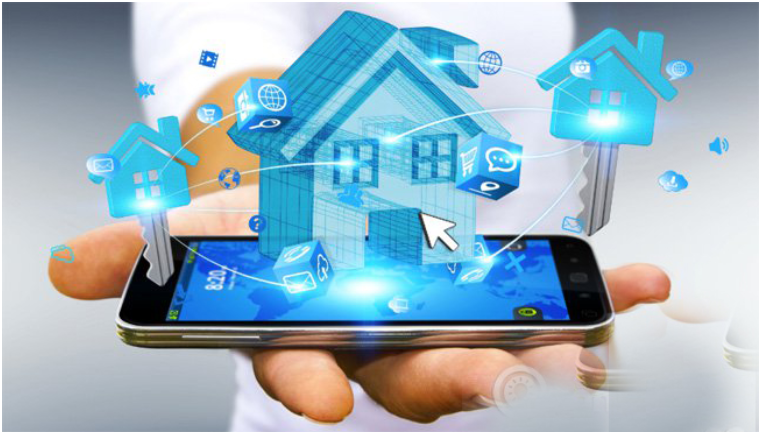
\includegraphics[scale=0.6]{image1/marthome.png}
    \end{center}
    \caption{Smarthome.}
    \label{refhinh1}
    \end{figure}
\end{center}
    \item Các thiết bị đeo thông minh\\
    Hiện nay ở nhiều nước đã xuất hiện các thiết bị đeo trên người với những tính năng vô cùng thông minh như: tai nghe, các loại kính, ba lô, vòng tay siêu thông minh,… Những thiết bị này dần bùng nổ tại các thị trường trên toàn thế giới. Google và Samsung là những công ty lớn có những khoản đầu tư khổng lồ cho việc tạo ra các thiết bị như vậy. Các thiết bị đeo được cài đặt cảm biến và các phần mềm thu thập dữ liệu, thông tin người dùng. Các thiết bị này bao gồm các yêu cầu về thể chất, sức khỏe và có tính giải trí cao. Điều kiện tiên quyết cho các thiết kế này là công suất cực thấp và kích thước nhỏ gọn, có tính thẩm mỹ cao.
\newpage
 \begin{center}
    \begin{figure}[htp]
    \begin{center}
     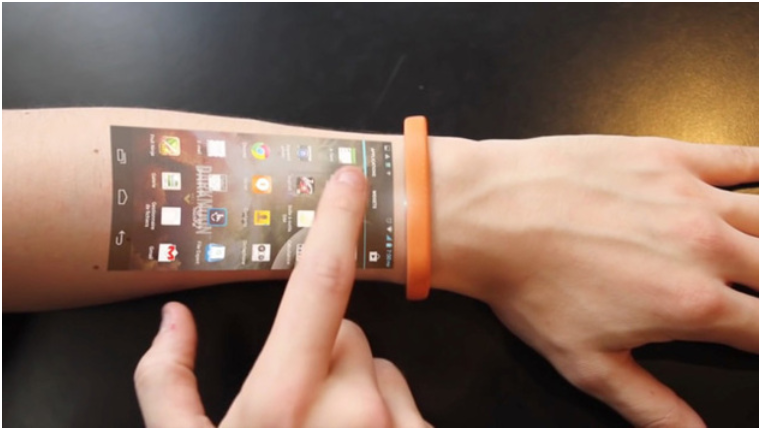
\includegraphics[scale=0.6]{image1/thietbi.png}
    \end{center}
    \caption{Thiết bị đeo tay thông minh.}
    \label{refhinh1}
    \end{figure}
\end{center} 
    \item Những chiếc ô tô được kết nối
 \begin{center}
    \begin{figure}[htp]
    \begin{center}
     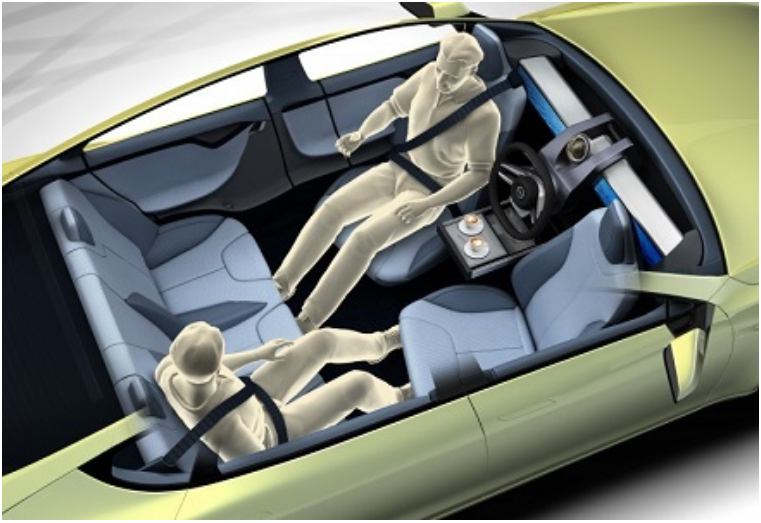
\includegraphics[scale=0.5]{image1/oto.png}
    \end{center}
    \caption{Ô tô thông minh.}
    \label{refhinh1}
    \end{figure}
\end{center} 
    Các nhà sản xuất ô tô đã bước qua giai đoạn tập trung vào việc tối ưu hóa các chức năng nội bộ của một chiếc xe. Giờ đây họ quan tâm đến việc tối ưu hóa sự hài lòng của người sử dụng với việc nâng cao trải nghiệm trong xe hơi.

    Một chiếc xe được kết nối là chiếc xe có khả năng tối ưu hóa hoạt động, bảo trì cũng như sự thoải mái của khách hàng khi sử dụng. Các thương hiệu lớn như BMW, Tesla, … đang nỗ lực cho cuộc cách mạng tiếp theo của ngành sản xuất ô tô.
    
    \item Internet công nghiệp
 \begin{center}
    \begin{figure}[htp]
    \begin{center}
     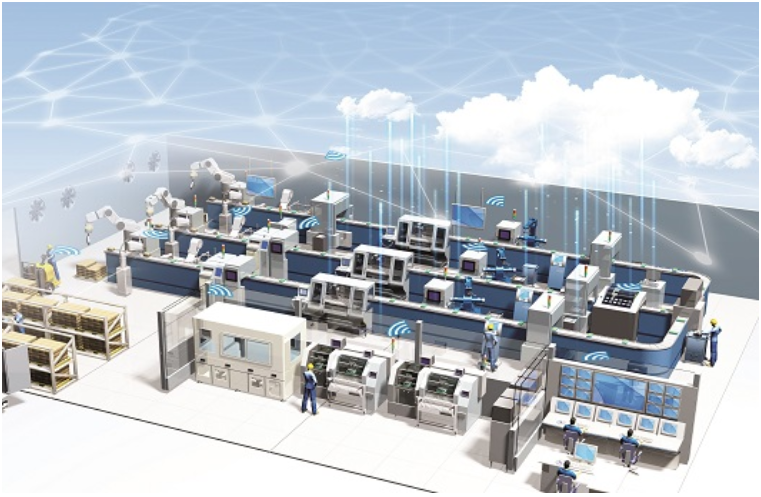
\includegraphics[scale=0.6]{image1/congnghiep.png}
    \end{center}
    \caption{Internet công nghiệp.}
    \label{refhinh1}
    \end{figure}
\end{center} 
    Industrial Internet là tiếng vang mới trong ngành công nghiệp, được gọi tắt là IIoT (Industrial Internet of Thing). IIoT hỗ trợ kĩ thuật công nghiệp với các cảm biến, phần mềm lớn để tạo ra những cỗ máy vô cùng thông minh. Máy móc sẽ có tính chính xác và nhất quán hơn con người trong giao tiếp thông qua dữ liệu. Từ những dữ liệu thu thập được giúp các công ty, nhà quản lí giải quyết các vấn đề sớm hơn, đạt hiệu quả cao hơn.

    IIoT có tiềm năng lớn về kiểm soát chất lượng và tính bền vững. Những ứng dụng trao đổi thông tin giữa nhà cung cấp, nhà phân phối và nhà bán lẻ về thông tin hàng hóa, hàng tồn kho sẽ làm tăng hiệu quả chuỗi cung ứng.
    
    \item Smart city
    Thành phố thông minh là một ứng dụng của IoT tạo được sự tò mò của đông dảo người dân. Giám sát thông minh, vận chuyển tự động, hệ thống quản lý năng lượng thông minh hơn, phân phối nước, an ninh đô thị và giám sát môi trường tất cả là ví dụ về internet của các ứng dụng cho thành phố thông minh. IoT giúp giải quyết các vấn đề gặp phải tại các thành phố lớn đó là ô nhiễm môi trường, tắc nghẽn giao thông và thiếu năng lượng. Một ví dụ có thể kể đến của các thiết bị được sử dụng truyền thông di động như: thùng rác thông minh, chúng sẽ gửi cảnh báo đến bộ phận vệ sinh môi trường khi cần dọn sạch.

    Bằng cách cài đặt ứng dụng và dùng các thiết bị thông minh chúng ta hoàn toàn có thể dễ dàng tìm thấy các cây xăng, siêu thị, quán ăn hay thậm chí là những bãi gửi xe miễn phí. Ngoài ra hệ thống điện cũng được bảo vệ bởi các cảm biến sẽ giúp phát hiện nhanh chóng các vấn đề gây nhiễu, trục trặc, hay các vấn đề về lắp đặt.
    
\begin{center}
    \begin{figure}[htp]
    \begin{center}
     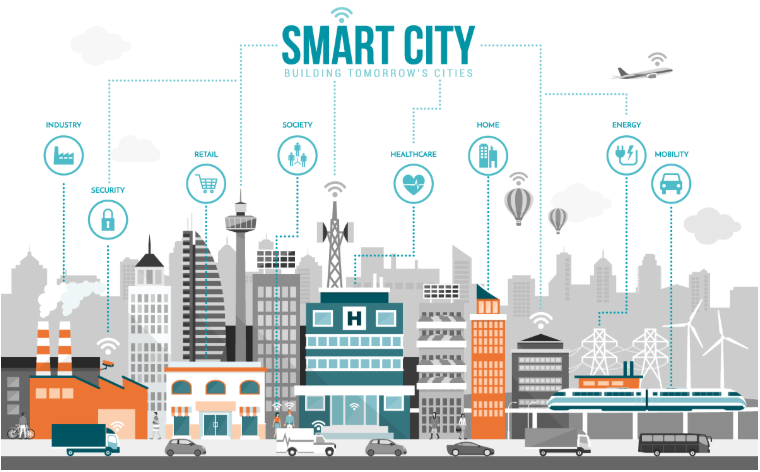
\includegraphics[scale=0.6]{image1/city.png}
    \end{center}
    \caption{Smart city.}
    \label{refhinh1}
    \end{figure}
\end{center} 
    \item IoT trong nông nghiệp
    Với sự gia tăng liên tục của dân số đồng nghĩa với việc nhu cầu sử dụng lương thực tăng lên nhiều lần. Nông dân có thể áp dụng các kỹ thuật mới, công nghệ tiên tiến để tăng sản lượng sản xuất nông nghiệp. Nông nghiệp thông minh có thể nói là lĩnh vực phát triển nhanh nhất với IoT.

    Những thông tin người nông dân thu được giúp họ có những quyết định đầu tư sáng suốt tránh tình trạng “được mùa mất giá, được giá mất mùa” như hiện nay. Cảm biến độ ẩm, chất dinh dưỡng của đất, mức độ hấp thụ nước góp phần quan trọng vào việc kiểm soát sự tăng trưởng của cây trồng giúp người gieo trồng có thể xác định, tùy chỉnh lượng phân bón cần thiết.
\begin{center}
    \begin{figure}[htp]
    \begin{center}
     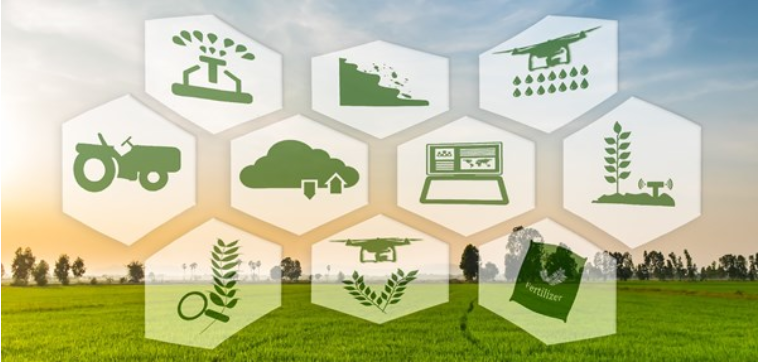
\includegraphics[scale=0.6]{image1/nongnghiep.png}
    \end{center}
    \caption{IoT trong nông nghiệp.}
    \label{refhinh1}
    \end{figure}
\end{center} 

    \item Bán lẻ thông minh
    IoT tạo nên một sự kết nối mật thiết giữa nhà bán lẻ với khách hàng giúp nâng cao trải nghiệm của khách hàng khi đến với cửa hàng. Tiềm năng phát triển IoT trong lĩnh vực bán lẻ là vô cùng lớn.

    Smart phone là thiết bị phổ biến nhất được sử dụng để các nhà bán lẻ duy trì kết nối với khách hàng của mình khi khách hàng đến với cửa hàng hay thậm chí ngay cả khi họ ra khỏi cửa hàng. Tương tác qua điện thoại và việc sử dụng các công nghệ giúp cho các nhà bán lẻ phục vụ khách hàng tốt hơn, thay đổi cách bài trí cửa hàng cho phù hợp với nhu cầu tiêu dùng.
\newpage 
\begin{center}
    \begin{figure}[htp]
    \begin{center}
     
\includegraphics[scale=0.6]{image1/banle.png}
    \end{center}
    \caption{Bán lẻ thông minh.}
    \label{refhinh1}
    \end{figure}
\end{center} 
    \item Năng lượng
\begin{center}
    \begin{figure}[htp]
    \begin{center}
     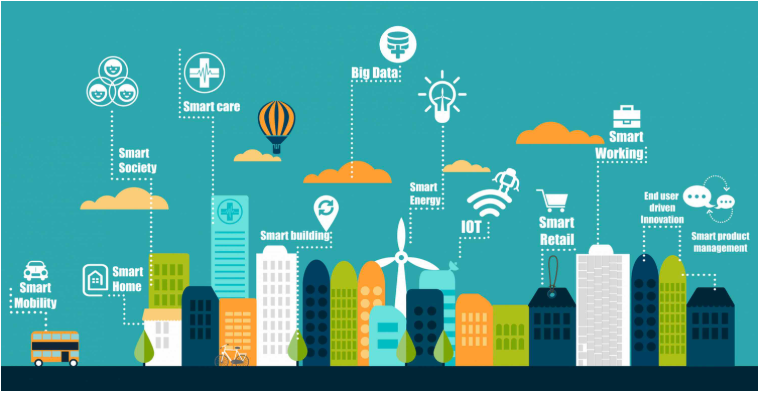
\includegraphics[scale=0.6]{image1/nangluong.png}
    \end{center}
    \caption{Năng lượng.}
    \label{refhinh1}
    \end{figure}
\end{center} 
    Mạng lưới điện trong vài năm tới sẽ trở nên thông minh và đáng tin cậy hơn. Khái niệm lưới điện thông minh đang trở nên phổ biến trên toàn thế giới.

    Dữ liệu được thu thập một cách tự động để phân tích hành vi tiêu dùng điện của người dùng và nhà cung cấp để góp phần nâng cao hiệu quả sử dụng điện. Lưới điện thông minh giúp phát hiện nguồn ngắt điện thông minh ở cấp độ các hộ gia đình.
    
    \item Sức khỏe
\begin{center}
    \begin{figure}[htp]
    \begin{center}
     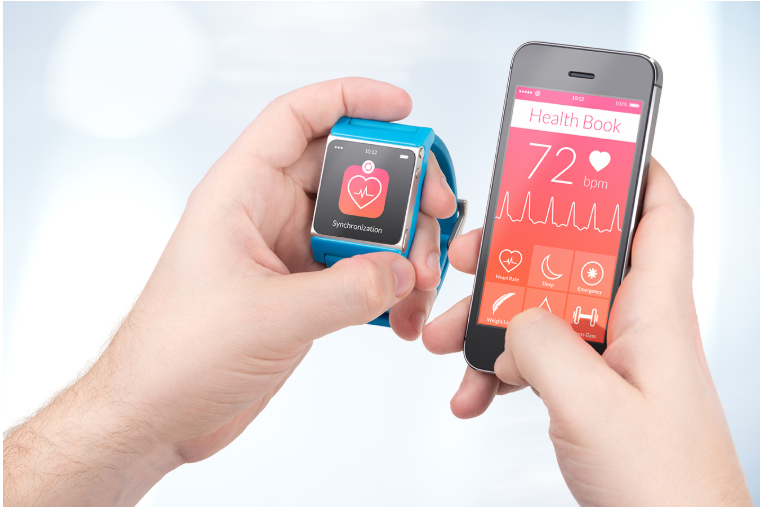
\includegraphics[scale=0.6]{image1/suckhoe.png}
    \end{center}
    \caption{Sức khỏe.}
    \label{refhinh1}
    \end{figure}
\end{center} 
    Đây có thể nói là một lĩnh vực chưa được khai phá hết của Internet of Things bởi những ứng dụng không ngờ mà nó mang lại. Một hệ thống chăm sóc sức khỏe được kết nối cùng các thiết bị y tế thông minh mang lại tiềm năng to lớn cho các công ty đầu tư sản xuất. IoT trong chăm sóc sức khỏe giúp mọi người có cuộc sống khỏe mạnh hơn bằng việc đeo các thiết bị kết nối. Các dữ liệu thu thập được giúp phân tích sức khỏe của người dùng thiết bị kết nối và nhà cung cấp, sản xuất sẽ có được những thiết kế để chống lại bệnh tật.
    
    \item IoT và chăn nuôi gia cầm, sản xuất nông trại.
    Kiểm soát các khâu trong quy trình chăn nuôi giúp tiết kiệm thời gian và chi phí. Sử dụng các công cụ IoT để thu thập dữ liệu về sức khỏe của gia súc, các chủ trang trại có thể biết sớm về bệnh tật của động vật giúp ngăn ngừa số lượng lớn các gia súc bị bệnh bởi virus lây lan. Với những dữ liệu thu thập được cũng giúp chủ trang trại tăng nhanh được sản lượng gia súc, gia cầm.

\begin{center}
    \begin{figure}[htp]
    \begin{center}
     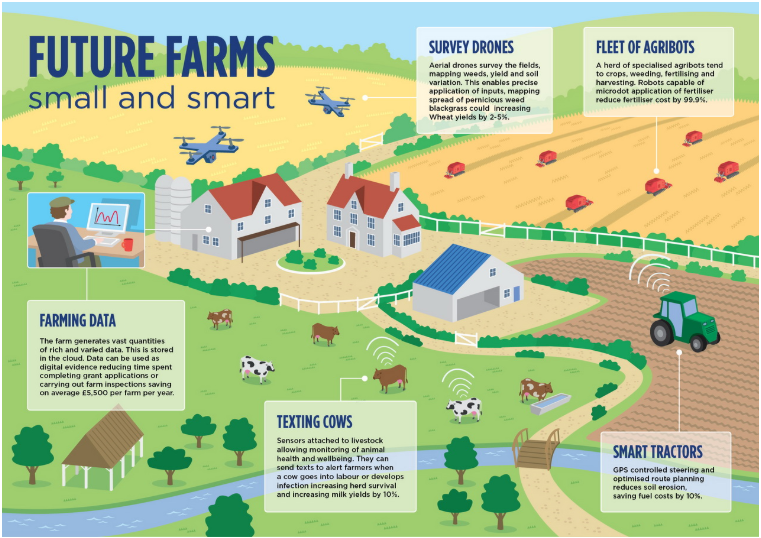
\includegraphics[scale=0.6]{image1/nongtrai.png}
    \end{center}
    \caption{IoT và chăn nuôi gia cầm, sản xuất nông trại.}
    \label{refhinh1}
    \end{figure}
\end{center} 
\end{enumerate}

Trong tương lai những gì IoT mang lại sẽ vượt xa những ứng dụng kể trên. IoT sẽ mang lại sự thay đổi tầm vĩ mô trong cách con người sống và làm việc\cite{tl13}.
\section{Các thách thức hiện tại của mạng IoTs}
Internet of Things - IoT có thể xem là đại diện của mọi thiết bị thông minh nhưng xu hướng này còn gặp nhiều khó khăn trong việc triển khai một cách toàn diện. IoT theo định nghĩa hiểu đơn giản là các bộ cảm biến có thể giao tiếp với Internet mà không cần có sự can thiệp của con người. Định nghĩa đó bao gồm cả các thiết bị đeo và điện thoại thông minh, hay các thiết bị có thể tự động giao tiếp nếu được cấp phép. IoT cũng bao gồm các thiết bị thông minh dành cho xe hơi, nhà ở và kể cả một thành phố hay thiết bị y tế hoặc công cụ trong các ngành công nghiệp. Những lợi ích và tiềm năng phát triển của IoT ở khắp mọi nơi, ở đâu có kết nối đều có khả năng xuất hiện các thiết bị với định danh của riêng mình, mang đến giá trị thông qua truyền tải, trao đổi thông tin, dữ liệu. Có thể thuật ngữ này sẽ biến mất khi IoT trở thành một chuẩn mực, và có thể được thay thế bằng một cái tên gọi khác nhằm ám chỉ những thiết bị không thể giao tiếp. Nhưng một số thách thức có thể làm trì hoãn tương lai của IoT và sau đây là những trở ngại đáng chú ý.\\
\begin{itemize}
\item \textbf{An ninh và bảo mật dữ liệu}: IoT đã trở thành một mốt quan tâm đáng lo ngại về an ninh, nó đã thu hút sự chú ý của các công ty công nghệ nổi tiếng và các cơ quan chính phủ trên toàn thế giới. Việc hack vào các thiết bị IoT như màn hình theo dõi em bé, tủ lạnh thông minh, máy bơm nước, điều hòa nhiệt độ, camera hay thậm chí là radio trong ô tô đang trở thành mối lo ngại về an ninh do sự phát triển của IoT gây ra. Vì vâỵ, các thiết bị mới được thêm vào mạng sẽ là yếu tố để các hacker có thể tấn công và xâm nhập dữ liệu trái phép vì số lượng lỗ hổng bảo mật là khá đáng kể.
Mọi vấn đề bảo mật chỉ tốt khi chúng ta có thể chỉ ra các điểm yếu của thiết bị, và đối với một thế giới kết nối như hiện nay thì điều đó có rất nhiều.\\

Điều này giải thích lý do tại sao Samsung đã dành nỗ lực đáng kể vào nền tảng ARTIK dành cho IoT trong thời gian gần đây. ARTIK có 3 mẫu module chứa tất cả các thành phần – bộ cảm biến, vi xử lý, bộ nhớ tích hợp, và kèm theo đó là khả năng kết nối không dây cần thiết cho các nhà sản xuất để tạo ra thiết bị thông minh. Tất cả các module ARTIK đều được hãng trang bị một khoá an toàn nhằm giúp các nhà phát triển mã hoá dữ liệu tốt hơn so với phần mềm mã hoá mặc định.\\

Đối với các thiết bị cá nhân có khả năng kết nối Internet thì vấn đề an ninh và sự riêng tư là những mối quan tâm hàng đầu. Đây có lẽ là những sản phẩm điển hình để được trang bị hệ thống mã hóa, nhưng vấn đề an ninh và sự riêng tư lại có đặc thù riêng khác nhau. An ninh bảo mật thường gằn liền với công nghệ còn sự riêng tư thì thương liên quan đến con người và tính pháp lý. Các nhà sản xuất thiết bị IoT cần phải hiểu rằng an ninh và sự riêng tư không thể đồng nhất hoặc áp dụng chung mọi quy tắc. Khả năng giao tiếp tự động của thiết bị IoT làm cho việc đảm bảo sự riêng tư khó khăn hơn bởi các mô hình sản phẩm được khuyến khích sử dụng trước khi có sự đồng thuận của người dùng ở những thời điểm khác nhau.\\

\item \textbf{Tiêu chuẩn chung}: Việc thiếu các tiêu chuẩn, đặc biệt là trường hợp sử dụng nhiều giao thức kết nối như hiện nay, là một cản trở cho IoT phát triển. Nhiều giao thức kết nối đặc biệt đang nổi lên với mức tiêu thụ năng lượng thấp như LTE Cat.0, 802.11ah, Sigfox hay OnRamp. Công nghệ bộ xử lý hiện cũng chưa thực sự hào hứng với thị trường IoT khi chuẩn giao thức không thực sự rõ ràng.\\

Các hãng công nghệ như LG, Panasonic, Sharp, Silicon Image, TP-Link, HTC, Qualcomm và hơn 100 thành viên khác đã thành lập nên liên minh AllSeen, dẫn đầu là Hiệp hội Linux. Tiêu chí của liên minh này là xóa bỏ những rào cản cũng như thúc đẩy sự sáng tạo trong việc phát triển Internet of Things. Nhóm này đã xây dựng nên nền tảng nguồn mở AllJoyn cho phép các sản phẩm IoT có thể giao tiếp với nhau thông qua nhiều dạng kết nối từ Wi-Fi, Ethernet, và cả đường dây điện. AllJoyn có thể tương thích với mọi hệ điều hành hiện nay và cũng không bắt buộc các thiết bị phải kết nối vào Internet bởi chúng có thể liên lạc ở cấp độ ngang hàng\\

Open Internet Consortium (OIC): Đây được xem là đối thủ của AllSeen Alliance, tổ chức OIC được các ông lớn công nghệ gồm Intel, Broadcom, Dell và Samsung chống lưng nhằm phát triển các tiêu chuẩn và chứng nhận cho các thiết bị Internet of Things. Các tiêu chuẩn này cũng xoay quanh khả năng giao tiếp và chứng thực thiết bị dựa trên các giao thức kết nối khác nhau gồm Wi-Fi, Bluetooth và cả NFC.\\

Thread Group: Tổ chức phi lợi nhuận này được thành lập bởi Nest Labs (thuộc Google), Samsung, ARM, Freescale, Silicon Labs... Thread Group tạo ra một giao thức mạng không dây dựa trên IP, cho phép các thiết bị phần cứng trong nhà kết nối với đám mây. Mục tiêu mà Thread Group còn nhắm đến việc giảm mức tiêu thụ năng lượng của thiết bị và đảm bảo tính an toàn bảo mật kết nối với IPv6. Tổ chức này dường như chỉ tập trung vào nền tảng hạ tầng hoạt động của IoT chứ không can thiệp quá nhiều vào phần cứng. Điều này cũng giúp dễ dàng tương thích với các tiêu chuẩn khác như AllSeen hay OIC.\\

Industrial Internet Consortium (IIC): Đây là tổ chức thứ 2 mà Intel tham gia vào nhằm phát triển IoT, ngoài ra General Electric, Cisco Systems, IBM và nhà mạng AT\&T là những thành viên thành viên tích cực nhất. Tuy nhiên, IIC tập trung vào mảng thiết bị IoT dùng cho doanh nghiệp và đảm bảo mọi thứ cùng hoạt động tốt ở mọi phân khúc thị trường. Ngoài ra, IIC giúp cải tiến các hệ thống máy móc lỗi thời có thể tham gia vào hệ thống IoT.\\

IEEE P2413: Viện kĩ thuật điện điện tử (IEEE) là một trong những tổ chức chính quy có nhiệm vụ đặt ra các tiêu chuẩn quan trọng trong thế giới công nghệ. Nhưng trong xu hướng IoT thì IEEE bị các công ty công nghệ cho rằng quá chậm chạp trong việc thiết lập tiêu chuẩn. IEEE quy tụ 23 nhà sản xuất có liên quan và cùng nghiên cứu tạo nên bộ chuẩn chung cho thiết bị.\\

\item \textbf{ Kết nối}: Kết nối rất nhiều thiết bị sẽ là một trong những thách thức lớn nhất của tương lai IoT, và sẽ phải tái cấu trúc các mô hình truyền thống hiện tại và công nghệ kết nối. Hiện tại, chúng ta đang dựa và mô hình tập trung, server-client để xác thực, ủy quyền các nút khác nhau trong một mạng.\\

Mô hình này là đủ cho hệ sinh thái IoT hiện tại, khi hàng chục, hàng trăm, hàng nghìn thiết bị kết nối. Nhưng khi IoT phát triển, hàng tỷ và hàng trăm tỷ thiết bị kết nối, hệ thống tập trung hiện tại sẽ bị thắt cổ chai. Các hệ thống lớn để đáp ứng số lượng lớn thiết bị này sẽ yêu cầu sự đầu tư khổng lồ vào các máy chủ đám mây để có thể xử lý lượng trao đổi thông tin khổng lồ.\\

IDC và EMC ước tính rằng tới năm 2020, sẽ có 44 nghìn tỉ gigabyte dữ liệu trên thế giới và 10 trong số đó là đến từ các thiết bị IoT. Mức này tương đương với 4.4 nghìn tỉ gigabyte, đồng thời cũng tương đương với mức dung lượng tất cả dữ liệu trên thế giới ước tính vào năm 2013. Nói cách khác, sức chứa của tất cả các trung tâm dữ liệu trực tuyến trong năm 2013 chỉ đủ để lưu trữ dữ liệu IoT trong năm 2020. Điều này sẽ có ảnh hưởng lớn tới cách các trung tâm dữ liệu làm việc để chúng có thể chịu được lượng dữ liệu lưu trữ trên đám mây khi các dữ liệu này được tạo ra và trao đổi.\\

\begin{figure}[htp]
\begin{center}
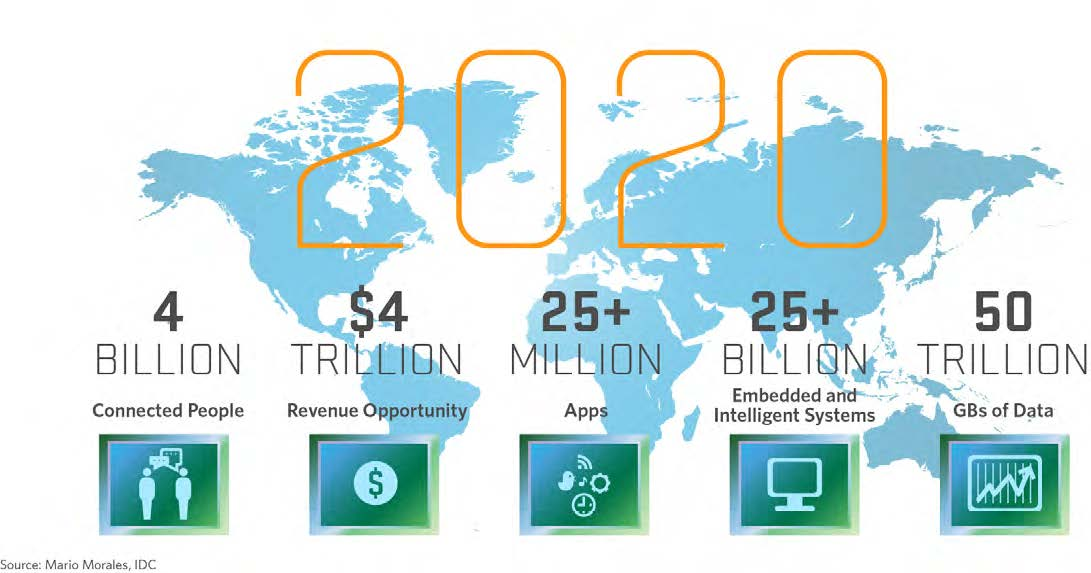
\includegraphics[scale=1]{image1/IoT.jpg}
\end{center}
\caption{Dự đoán IoT đến năm 2020}
\label{IoT2020}
\end{figure}
\newpage
Còn quan trọng hơn cả là yêu cầu kết nối để giúp tất cả các thiết bị này giao tiếp với nhau, để có thể gửi dữ liệu đến và đi khỏi kho lưu trữ dữ liệu trực tuyến. Giao thức IPv6 được tạo đã phần nào nghĩ tới tương lai này khi nó hỗ trợ $2^{128}$ địa chỉ, so với chỉ $2^{32}$ địa chỉ của giao thức IPv4. Lưu lượng dữ liệu trên 1 thiết bị cá nhân có thể không quá nhiều. Bluetooth cũng có thể đủ dùng với nhiều mạng cảm biến đòi hỏi mức năng lượng thấp, và rất nhiều trong số này cũng được tải lên rải rác chứ không stream mọi thông tin cùng 1 lúc.\\

Thế nhưng, tổng hợp hàng tỉ thiết bị trực tuyến vào năm 2020 và tất cả lượng băng thông sẽ là rất lớn. Quản lý dung lượng kết nối mạng một cách cẩn trọng sẽ là việc vô cùng thiết yếu.
\end{itemize}

\section{Giới thiệu đề luận văn}
Với sự phát triển của Internet of Things (IoTs), rất nhiều ứng dụng tiện ích đã được hiện thực. Tuy nhiên, các ứng dụng hiện tại đều tập trung vào việc gửi dữ liệu trực tiếp từ node cảm biến về node trung tâm. Điều này làm cản trở việc triển khai ứng dụng trên diện rộng, khi tầm bao phủ của ứng dụng lớn hơn phạm vi gửi dữ liệu không dây. Do đó, việc phát triển một nền tảng cho phép gửi dữ liệu qua nốt trung gian (multi-hop) sẽ mở ra nhiều cơ hội cho việc triển khai ứng dụng. Bên cạnh đó, node trung tâm cũng cần dựa trên một hệ điều hành, thay vì chủ yếu là nền tảng vi điều khiển như hiện tại, để có thể hỗ trợ nhiều xử lý đa dạng và phức tạp (ví dụ: kết nối 3G, cập nhật firmware từ xa) cũng như nâng cao độ ổn định của hệ thống.\\
\subsection{Mục tiêu của luận văn}
Xây dựng hệ thống thu thập dữ liệu trên nền tảng mạng cảm biến không dây multi-hop và hệ điều hành nhúng phục vụ cho ứng dụng Internet of Things.
\subsection{Mục tiêu cụ thể của giai đoạn thực tập}
Tìm hiểu các chuẩn giao tiếp không dây hiện có, lựa chọn tiêu chuẩn giao tiếp phù hợp dựa vào các tiêu chí: tầm xa, năng lượng, độ ổn định (tỉ lệ lỗi thấp).
\newline
Tìm hiểu các hệ điều hành nhúng đang được hỗ trợ phổ biến cho các mạng cảm biến IoTs (ví dụ: Android things, Windows things,…). Lựa chọn hệ điều hành phù hợp cho đề tài.
\subsection{Các ứng dụng tiềm năng cho kết quả của luận văn}
Xây dựng một ứng dụng giám sát trên phạm vi rộng (ví dụ môi trường nước hoặc môi trường không khí) để kiểm tra tính đúng đắn của đề tài.





\chapter{Kiến trúc tổng quan của hệ thống}
\section{Giới thiệu}
\begin{figure}[ht]
\begin{center}
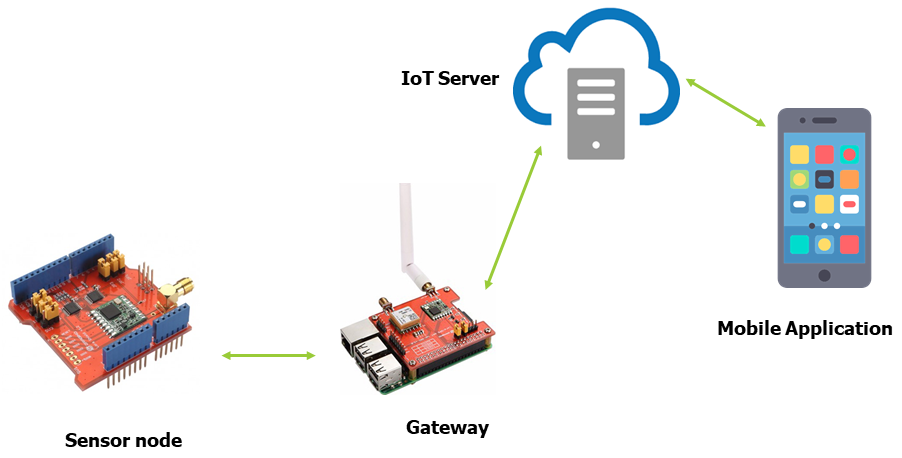
\includegraphics[scale=0.6]{image2/gioi-thieu-chuong-2.png}
\end{center}
\caption{Kiến trúc tổng quan hệ thống}
\end{figure}
Hệ thống Lora được sử dụng trong IOT vì LoRa có thể được áp dụng rộng rãi trong các ứng dụng thu thập dữ liệu như sensor network trong đó các sensor node có thể gửi giá trị đo đạc về trung tâm cách xa hàng km và có thể hoạt động với battery trong thời gian dài trước khi cần thay pin .Một đặc thù riêng biệt, ở môi trường nông nghiệp thì việc truyền dữ liệu từ các cảm biến và trung tâm, và từ trung tâm tới các thiết bị chấp hành sẽ gặp phải các khó khăn về khoảng cách, dễ bị tác động của môi trường,...dẫn đến hệ thống không hoạt động ổn định. Ngoài Zigbee, LoRa là một lựa chọn tuyệt vời. 
Về tổng quan hệ thống bao gồm:
\begin{enumerate}
    \item Các sensor node bao gồm 1 board lora và 1 board arduino. Các node này có nhiệm vụ truyền nhận dữ liệu trong mạng. Giúp dữ liệu từ các cảm biếm có thể đến gateway.
    \item Gateway bao gồm 1 Lora và 1 raspbery. với khả năng tính toán của raspberry thì sẽ đẩy được nhiều dữ liệu lên server cùng một lúc.
    \item Server trức mắt sử dung mqtt.MQTT (Message Queuing Telemetry Transport) là một giao thức gởi dạng publish/subscribe sử dụng cho các thiết bị Internet of Things với băng thông thấp, độ tin cậy cao và khả năng được sử dụng trong mạng lưới không ổn định.

    Bởi vì giao thức này sử dụng băng thông thấp trong môi trường có độ trễ cao nên nó là một giao thức lý tưởng cho các ứng dụng M2M.
    
    \item Application là điện thoại hoặc PC. Giúp người dùng theo dõi dữ liệu trong hệ thống mạng.
\end{enumerate}

\section{Kiến trúc hệ thống}
Hệ thống bao gồm các gateway được đặt ở những nơi có điện và có khả năng kết nối internet. Vì gateway tiếp nhận nhiều dữ liệu nên tiêu tốn nhiều điện cần đặt ở nơi có nguồn điện ổn định.Internet để kết nối lên server.\\
Gateway sẽ kết nối dữ liệu với các node xung quanh để truyền dữ liệu, cấp ID, giúp tìm đường truyền...Các node sẽ thực hiện kết nối với các node xung quanh sao cho dữ liệu truyền đi là tốt nhất.
\newpage
\begin{figure}[ht]
\begin{center}
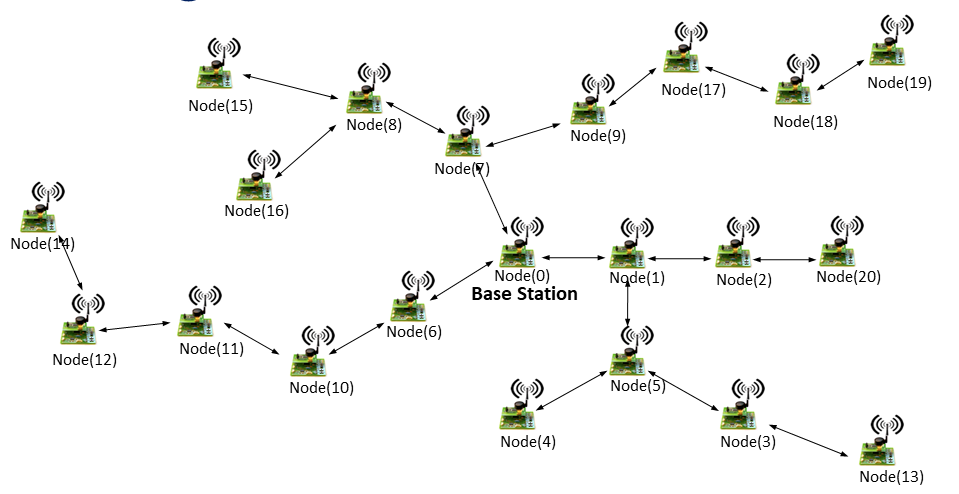
\includegraphics[scale=0.6]{image2/kien-truc-he-thong.png}
\end{center}
\caption{Kiến trúc hệ thống}
\end{figure}

\section{Kiến trúc node cảm biến}

\begin{center}
    \begin{figure}[htp]
    \begin{center}
     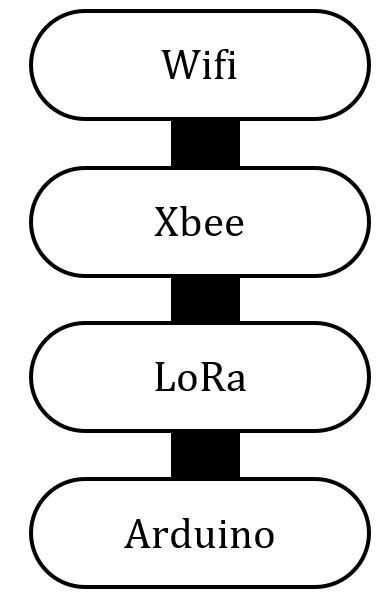
\includegraphics[scale=0.4]{image2/node.JPG}
    \end{center}
    \caption{Kết nối với node cảm biến.}
    \end{figure}
\end{center}

Bao gồm 4 module chính:
\begin{itemize}
    \item Wifi - module giao tiếp không dây, sử dụng mạng wifi. Dùng để cập nhật firmware cho các node cảm biến.
    \item Xbee - module giao tiếp không dây, sử dụng tín hiệu radio có tần sóng ngắn. Dùng để cập nhật firmware cho các node cảm biến.
    \item LoRa - module giao tiếp không dây, sử dụng tín hiệu sóng vô tuyến (radio) với dải băng tần không được cấp phép (433MHz). Dùng để gửi dữ liệu từ các node cảm biến đo đạc được bằng các sensor được gắn trên đó.
    \item Raspberry Pi 3 - Android Things, điều khiển các hoạt động của LoRa (gửi/nhận dữ liệu, quản lý các node cảm biến trong mạng lưới). Đồng thời xử lý dữ liệu nhận được theo chuẩn đã quy định trước khi đưa tất cả dữ liệu lên server.
\end{itemize}

\section{Kiến trúc node gateway}

\begin{center}
    \begin{figure}[htp]
    \begin{center}
     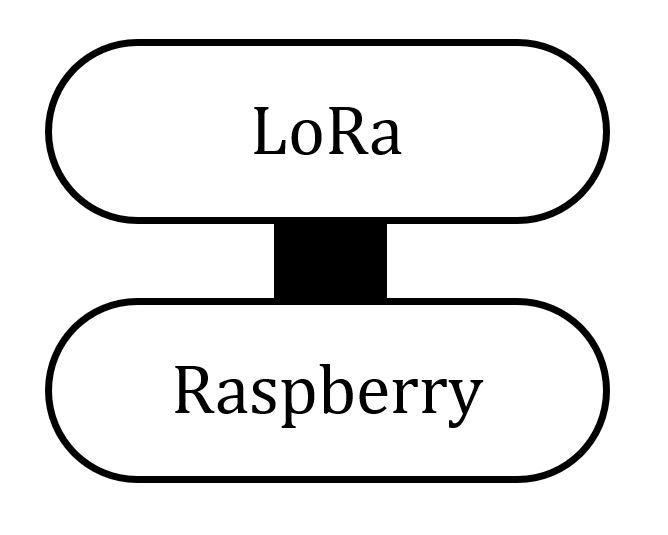
\includegraphics[scale=0.3]{image2/gateway.JPG}
    \end{center}
    \caption{Kết nối với node gateway.}
    \end{figure}
\end{center}

Bao gồm 2 module chính:
\begin{itemize}
    \item LoRa - module giao tiếp không dây, sử dụng tín hiệu sóng vô tuyến (radio) với dải băng tần không được cấp phép (433MHz). Dùng để thu thập dữ liệu từ các node cảm biến đo đạc được bằng các sensor được gắn trên đó.
    \item Raspberry Pi 3 - Android Things, điều khiển các hoạt động của LoRa (gửi/nhận dữ liệu, quản lý các node cảm biến trong mạng lưới). Đồng thời xử lý dữ liệu nhận được theo chuẩn đã quy định trước khi đưa tất cả dữ liệu lên server.
\end{itemize}
 
\section{Mô hình giao tiếp không dây}
\subsection{Giao tiếp ở gateway}
\begin{enumerate}
    \item Ban đầu, Gateway sẽ kết nối với tât cả các node có cường độ tín hiệu thu(RSSI) lớn hơn -70dbm.
\begin{center}
    \begin{figure}[htp]
    \begin{center}
     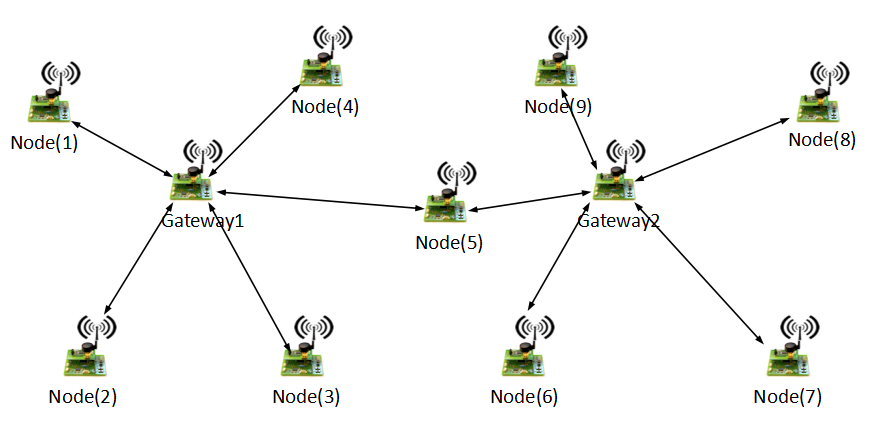
\includegraphics[scale=0.45]{image2/bandau.png}
    \end{center}
    \caption{Gateway kết nối với các node ban đầu.}
    \label{refhinh1}
    \end{figure}
\end{center}
    
    \item Giả sử Node có kết nối với 2 Gateway, thì nó sẽ thực hiện kết nối với node có cường độ tín hiệu thu lớn hơn.
\begin{center}
    \begin{figure}[htp]
    \begin{center}
     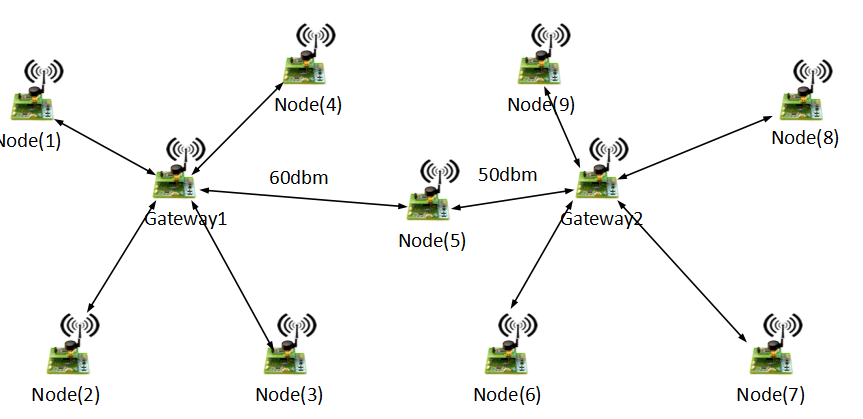
\includegraphics[scale=0.45]{image2/node5.png}
    \end{center}
    \caption{node(5) kết nối với hai Gateway.}
    \label{refhinh1}
    \end{figure}
\end{center}
\newpage
\item với các node ở xa, cường độ tín hiệu thu thấp, nhung không kết nối được với node trung gian nào khác, thì bây giờ thực hiện kết nối với gateway.
\begin{center}
    \begin{figure}[htp]
    \begin{center}
     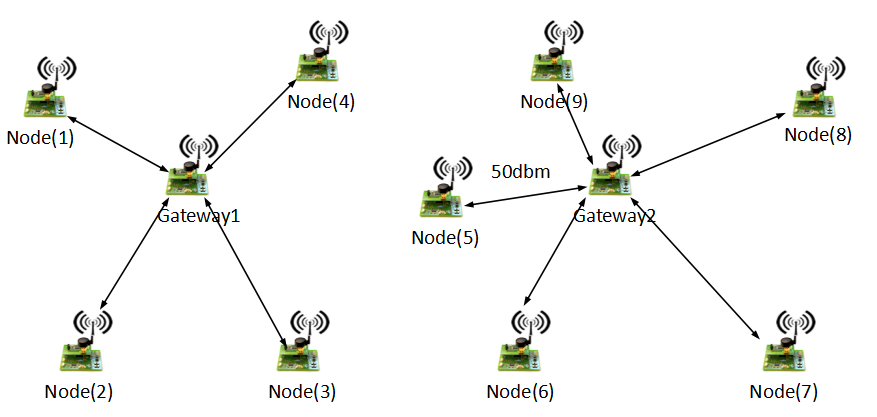
\includegraphics[scale=0.45]{image2/node51.png}
    \end{center}
    \caption{node(5) ngắt kết nối với Gateway1.}
    \label{refhinh1}
    \end{figure}
\end{center}

\item Gateway sẽ cấp địa chỉ IP cho các nối kết nối với nó. Và liên tục cập nhất các node mới, đồng thời kiển tra xem có tất cả có bao nhiêu node kết nối với nó.
\begin{center}
    \begin{figure}[htp]
    \begin{center}
     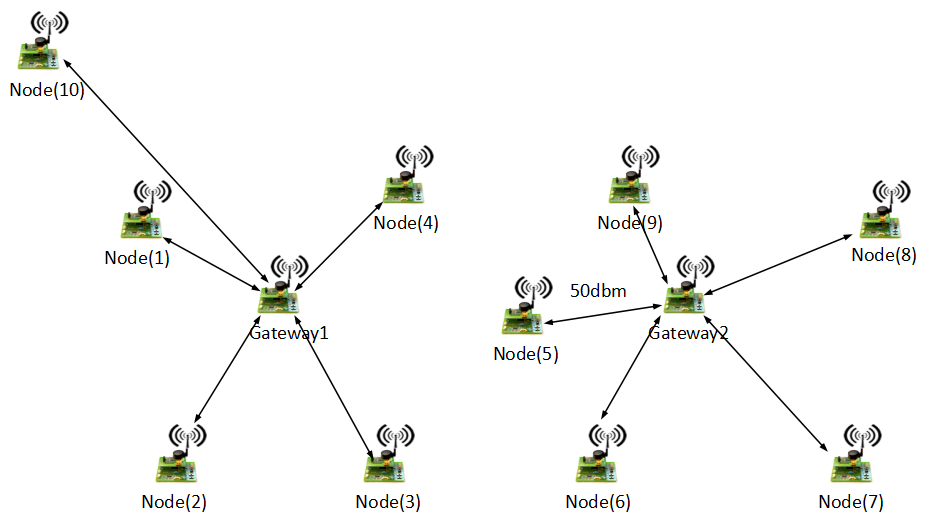
\includegraphics[scale=0.45]{image2/nodexa.png}
    \end{center}
    \caption{các node ở xa kết nối với Gateway.}
    \label{refhinh1}
    \end{figure}
\end{center}
 
    
\end{enumerate}

\subsection{Giao tiếp ở các node}
\begin{enumerate}
    \item các node chưa có kết nối gửi lên Gateway, thì nó sẽ gửi dữ liệu đi đến các node khác, kiển tra xem node đó đã kết nối hay chưa, rồi dựa vào các thông số như cường độ thu tín hiệu, số node trung gian cần phải qua để đến được gateway, số node hiện tại gateway đã kết nối,rồi quyết định kết nối với node phù hợp nhất.

\begin{center}
    \begin{figure}[htp]
    \begin{center}
     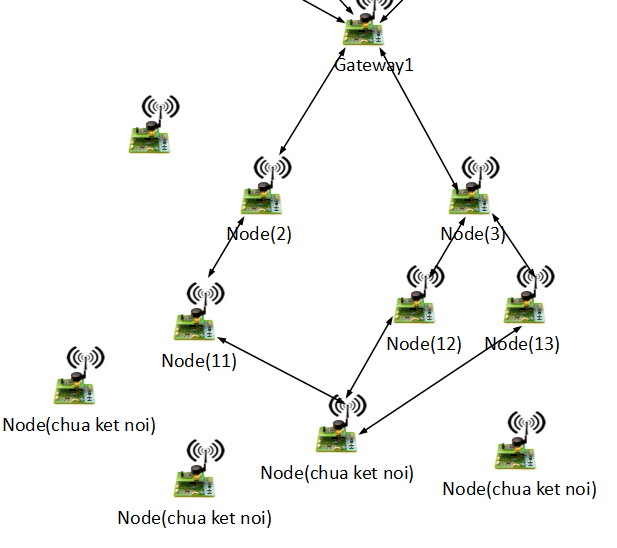
\includegraphics[scale=0.45]{image2/chuaketnoi.png}
    \end{center}
    \caption{Bắt tín hiệu các Gateway bên cạnh.}
    \label{refhinh1}
    \end{figure}
\end{center}

\begin{center}
    \begin{figure}[htp]
    \begin{center}
     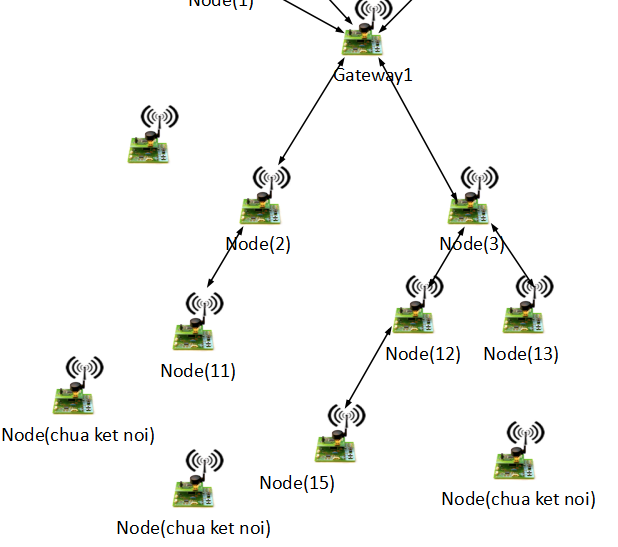
\includegraphics[scale=0.45]{image2/daketnoi.png}
    \end{center}
    \caption{Kết nối với node phù hợp.}
    \label{refhinh1}
    \end{figure}
\end{center}
\end{enumerate}

\chapter{Gateway IoTs dựa trên nền tảng Android Things}
\label{chapter3}
\section{Tại sao phải cần hệ điều hành?}
"Để đạt được giá trị từ Internet of Things (IoT), việc cần phải có một nền tảng (platform) để tạo và quản lý ứng dụng, chạy các phân tích, lưu trữ và bảo mật dữ liệu của bạn là một điều cần thiết. Giống như một hệ điều hành dành cho máy tính xách tay, một nền tảng làm rất nhiều thứ đằng sau đó, giúp cho cuộc sống của các nhà phát triển, nhà quản lý và người dùng dễ dàng hơn và ít tốn kém hơn."\cite{tl4}

\subsection{Vậy nền tảng (platform) là gì?}
"Nói chung, nền tảng (platform) là phần mềm và phần cứng, có thể bao gồm môi trường hoạt động, lưu trữ, sức mạnh máy tính, bảo mật, công cụ phát triển và nhiều chức năng phổ biến khác. Nền tảng được thiết kế để hỗ trợ nhiều chương trình ứng dụng nhỏ hơn mà thực sự giải quyết các vấn đề kinh doanh.\\

Nền tảng hữu ích vì chúng rút ra rất nhiều chức năng chung từ logic ứng dụng cụ thể. Ví dụ, bất kể bạn đang cố gắng viết một ứng dụng để tối ưu hoá mức tiêu hao nhiên liệu hoặc không gian lớp học, cơ bản bạn cần khá nhiều công nghệ giống nhau. Các nhà phát triển ứng dụng chỉ muốn tập trung vào vấn đề cụ thể mà họ đang giải quyết và sử dụng các khả năng chung để tính toán sức mạnh hoặc lưu trữ hoặc bảo mật. Một nền tảng tốt làm giảm đáng kể chi phí phát triển và duy trì các ứng dụng.\\

Trong Internet of Things, các nền tảng được thiết kế để triển khai các ứng dụng giám sát, quản lý và kiểm soát các thiết bị được kết nối (hình bên dưới). Các nền tảng IoT phải xử lý các vấn đề như kết nối và trích xuất dữ liệu từ một số lượng khổng lồ các điểm cuối khác nhau, đôi khi ở các vị trí không thuận tiện với kết nối chập chờn."\cite{tl4}
\subsection{Vậy hệ điều hành là gì?}
Hệ điều hành chính là một nền tảng phần mềm. Chi tiết hơn, nó là một môi trường hoạt động, được thiết kế để hỗ trợ cho các chương trình ứng dụng, hoặc thấm chí là công cụ phát triển.\cite{tl5}\\

Tuy nhiên, với hệ điều hành dành cho IoT sẽ khó sử dụng cho nhiều mục đích hoặc ứng dụng hàng hoạt trên mọi sản phẩm, bởi vậy cần có nhiều hệ điều hành khác nhau trong lĩnh vực IoT để đáp ứng nhu cầu thực tế.\cite{tl5}

\subsection{Tại sao lại cần đến hệ điều hành?}
Trong đề tài luận văn này, hệ điều hành IoT được lựa chọn phải ít phức tạp hơn, đòi hỏi khả năng xử lý dữ liệu có độ trễ thấp nhất có thể, nhưng vẫn có đầy đủ khả năng và đáp ứng được các yêu cầu về tiêu thụ năng lượng, không đòi hỏi nhiều về tài nguyên như bộ xử lý hay bộ nhớ RAM.\cite{tl5}\\

Việc sử dụng hệ điều hành sẽ giúp cho việc cập nhật firmware một cách dễ dàng, thông qua mạng internet - wifi (hoặc công nghệ truyền không dây ZigBee), nếu trong mạng lưới có tới hàng trăm thiết bị đều cần phải cập nhật. Ngoài ra, hệ điều hành sẽ giúp tăng tính bảo mật, tăng sức mạnh, khả năng lưu trữ cho các thiết bị IoT. Đồng thời sẽ giúp quản lý được năng lượng sử dụng.\\

Vậy nên, nhóm đã quyết định sử dụng hệ điều hành Android Things trong đề tài này. Vì hiện nay, Android Things đang phát triển và nhận được sự hỗ trợ rất lớn của Google và cộng đồng mạng (cồng đồng phát triển trên nền tảng Android).

\section{Giới thiệu hệ điều hành Android Things}
"Android things là hệ điều hành được quản lý bởi Google dựa trên nền tảng Android cho phép bạn có thể xậy dựng những ứng dụng IoT mà bạn không cần phải có quá nhiều kiến thức về hệ thống nhúng."\cite{tl6}
\\
"Về cơ bản, Android Things là một bản cập nhật và làm mới lại của Brillo, hệ điều hành dựa trên nền tảng Android dành cho các thiết bị thông minh và các sản phẩm Internet of Things (IoT) được giới thiệu vào năm 2015."\cite{tl7}
\\
"Android Things là một phiên bản rút gọn của Android có thể chạy trên những nguyên mẫu phần cứng khác nhau, để dễ dàng tạo ra thiết bị kết nối Internet of Things (IoT). Điều này làm cho mã nhúng có thể được truy cập đối với các nhà phát triển những người có thể không có kinh nghiệm trước đó. Với Android Things, Google cũng cung cấp một thư viện mà bạn có thể sử dụng để xây dựng các ứng dụng đọc từ và ghi vào các chân nối khác nhau trên bảng mạch, cho phép bạn đấu vào đó các cảm biến và bộ thiết bị điều tiết khác nhau để tương tác với thế giới."\cite{tl8}

\section{Tại sao nên sử dụng Android Things?}
\begin{itemize}
\item Do Android Things là một phân mở rộng của nền tảng Android neen bạn hoàn toàn có thể sử dụng các tool đã quen thuộc với Android Developer như Android Studio và Android SDK để phát triển chúng.
\item Android Things OS được quản lý bởi Google nên nó an toàn.
\item Được hỗ trợ trong hệ sinh thái phong phú của Google : Google Cloud, Tensor Flow, Play Services, Assistant SDK, Firebase...
\item Bạn có thể sử dụng những ngôn ngữ lập trình High-Level như Java, Kotlin để xây dưng ứng dụng IoT.\cite{tl6}
\end{itemize}

\section{Các nền tảng nhúng hỗ trợ Android Things}
"Tại thời điểm này, Android Things hỗ trợ ba nguyên mẫu phần cứng: 
\begin{itemize}
\item Raspberry Pi 3 Model B (hoặc Raspberry Pi 2).
\item Edison Intel cùng với bo mạch Arduino.
\item NXP Pico i.MX6UL.
\end{itemize}
Mặc dù điều này có vẻ như là một sự hạn chế, nhưng một danh sách hạn chế các phần cứng cho phép Google hỗ trợ đầy đủ các nguyên mẫu bo mạch phổ biến và cung cấp cho các nhà phát triển một nền tảng vững chắc đã được thử nghiệm và kiểm chứng.\\

Ngoài ba bảng mạch đã đề cập, Android Things sẽ sớm hỗ trợ Intel Joule 570x và NXP Argon i.MX6UL, đem lại cho bạn nhiều tùy chọn phần cứng cho sự phát triển."\cite{tl8}

 \section{Xây dựng ứng dụng đầu tiên với Androids Things}
 Để xây dụng ứng dụng với Android Things cần phải đáp ứng một số yêu cầu sau,\\
 Về phần mềm:
 \begin{itemize}
 \item Môi trường \href{https://www.oracle.com/technetwork/java}{Java}.
 \item Ứng dụng lập trình Android (\href{https://developer.android.com/studio/}{Android Studio}).
 \item Và một số ứng dụng phụ khác khi mới bắt đầu sử dụng: 	\href{https://sourceforge.net/projects/win32diskimager/}{Win32 Disk Imager}/\href{https://www.balena.io/etcher/}{Etcher}, \href{https://www.sdcard.org/downloads/formatter_4/}{SD Card Formatter}, hoặc \href{https://partner.android.com/things/console/#/tools}{android-things-setup-utility}.
 \item Trình duyệt web \href{https://www.google.com/chrome}{Google Chrome} \textit{(khuyên dùng)}.
 \end{itemize}
 Về phần cứng:
 \begin{itemize}
 \item \href{https://www.raspberrypi.org/products/raspberry-pi-3-model-b/}{Raspberry Pi 3 Model B}.
 \item Thẻ nhớ MicroSD (từ 8GB trở lên).
 \item Đầu đọc thẻ nhớ MicroSD.
 \item Nguồn 5V – 2.5A (khuyên dùng). 
 \item Và một số thiết bị phần cứng khác khi mới bắt đầu sử dụng: màn hình HDMI/cảm ứng, cáp HDMI, chuột, bàn phím rời, cáp Ethernet (nếu không có sẵn mạng wifi).
 \end{itemize}
 \subsection{Cài đặt JDK}
 JDK là một bộ công cụ phát triển Java, nó dành cho những người lập trình Java để phát triển ứng dụng. Về cơ bản nó bao gồm:
 \begin{enumerate}
     \item JRE (Java Runtime Environment) là một môi trường chạy ứng dụng Java.
     \item Javac: Một chương trình để dịch mã mà bạn viết thành mã bytecode, khi ứng dụng Java chạy nó dịch mã bytecode thành mã máy tính và thực thi, điều đó có nghĩa là bytecode chỉ là một mã trung gian.
     \item Archive (jar): Là một chương trình nén các file thành một file duy nhất có đuôi jar. Thường dùng để đóng gói các file class.
     \item Javadoc: Là một công cụ tạo ra tài liệu hướng dẫn sử dụng API.
     \item Và các công cụ khác cần thiết cho phát triển Java.
 \end{enumerate}
 
 Để tiến hành cài đặt JDK chúng ta thực hiện các bước sau.
 \begin{enumerate}
     \item Vào đường dẫn \url{https://www.oracle.com/technetwork/java/javase/downloads/index.html} để download JDK
     \item nhấn vào Oracle JDK để chọn JDK cần download
\begin{center}
    \begin{figure}[htp]
    \begin{center}
     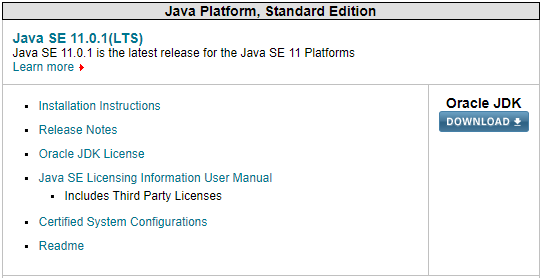
\includegraphics[scale=1.0]{image3/OracleJDK}
    \end{center}
    \caption{Oracle JDK}
    \label{refhinh1}
    \end{figure}
\end{center}
    \item nhấn chọn Accept License Agreement và sau đó chọn phiên bản phù hợp với hệ điều hành mà bạn đang sử dụng
\begin{center}
    \begin{figure}[htp]
    \begin{center}
     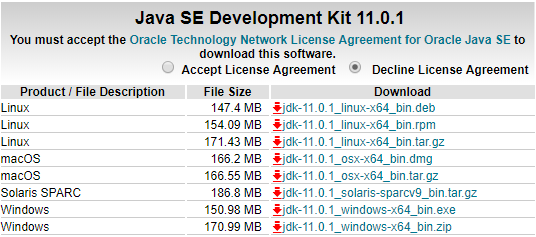
\includegraphics[scale=1.0]{image3/JDK}
    \end{center}
    \caption{Chọn Phiên bản JDK}
    \label{refhinh1}
    \end{figure}
\end{center}
\newpage
    \item Kết quả download được:
\begin{center}
    \begin{figure}[htp]
    \begin{center}
     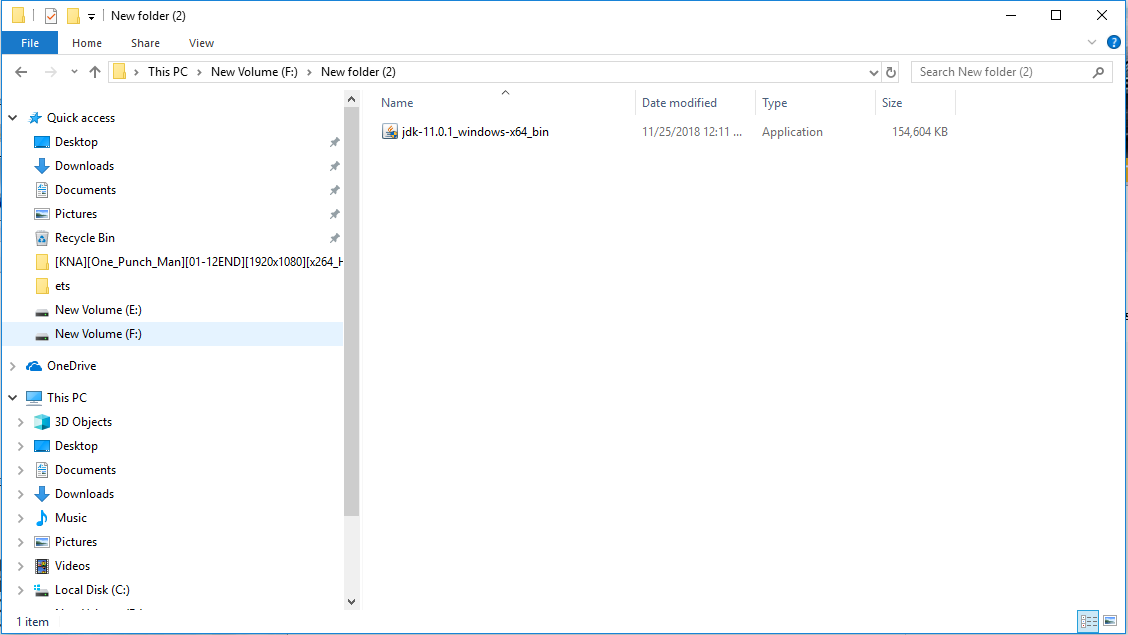
\includegraphics[scale=0.5]{image3/downloadjdk}
    \end{center}
    \caption{File JDK tải về}
    \label{refhinh1}
    \end{figure}
\end{center}
    \item chạy file vừa download về, nhấn next để tiếp tục.
\newpage
\begin{center}
    \begin{figure}[htp]
    \begin{center}
     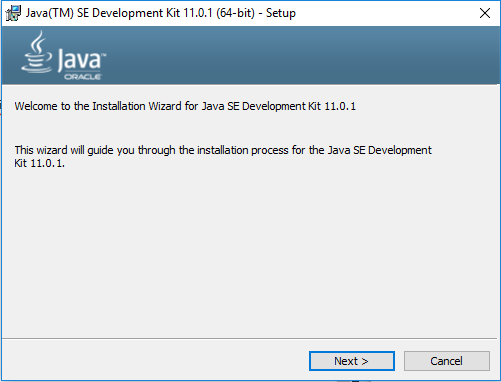
\includegraphics[scale=1.0]{image3/jdksetup}
    \end{center}
    \caption{Chạy File JDK tải về}
    \label{refhinh1}
    \end{figure}
\end{center}
    \item Nhập vào thư mục mà JDK sẽ được cài đặt ra, ở đây tôi đặt là: \textsf{C:Program File/Java/jdk-11.0.1/}
\newpage
\begin{center}
    \begin{figure}[htp]
    \begin{center}
     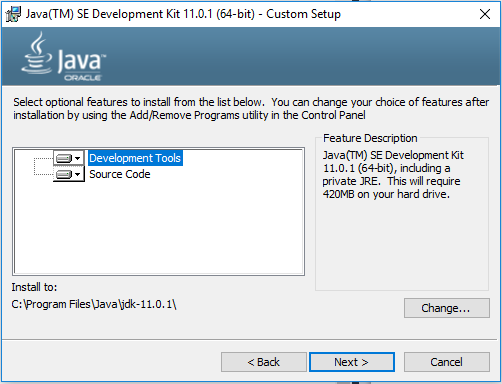
\includegraphics[scale=1.0]{image3/javatm}
    \end{center}
    \caption{Cài đặt đường dẫn file JDK tải về}
    \label{refhinh1}
    \end{figure}
\end{center}
    \item Nhấn next để tiếp tục, sau khi cài đặt xong nhấn close.
    \item Nhấn phải chuột vào Computer, chọn Properties. Sau đó nhấn Advance System Settings. Chon tiếp Advanced. Chọn Environment variables.
\newpage
\begin{center}
    \begin{figure}[htp]
    \begin{center}
     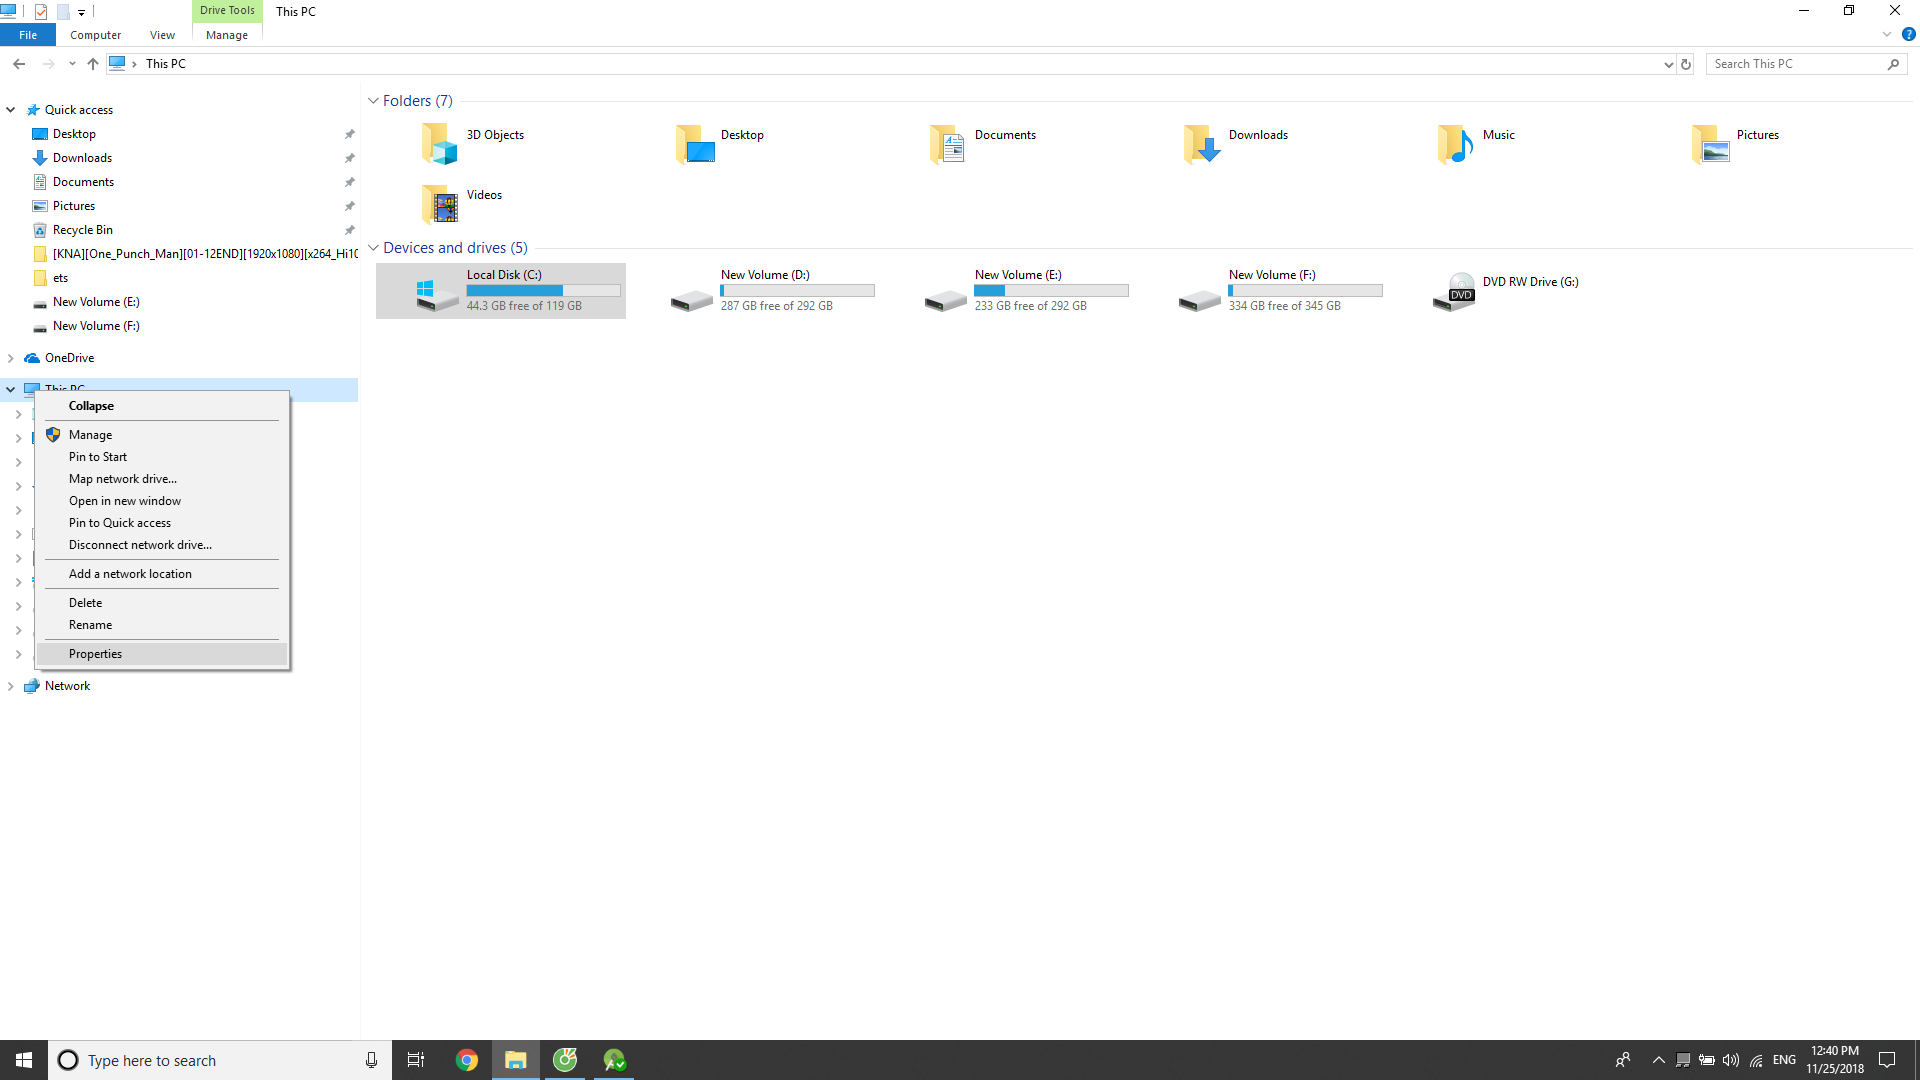
\includegraphics[scale=0.25]{image3/pc}
    \end{center}
    \caption{Chọn Properties.}
    \label{refhinh1}
    \end{figure}
\end{center}
\begin{center}
    \begin{figure}[htp]
    \begin{center}
     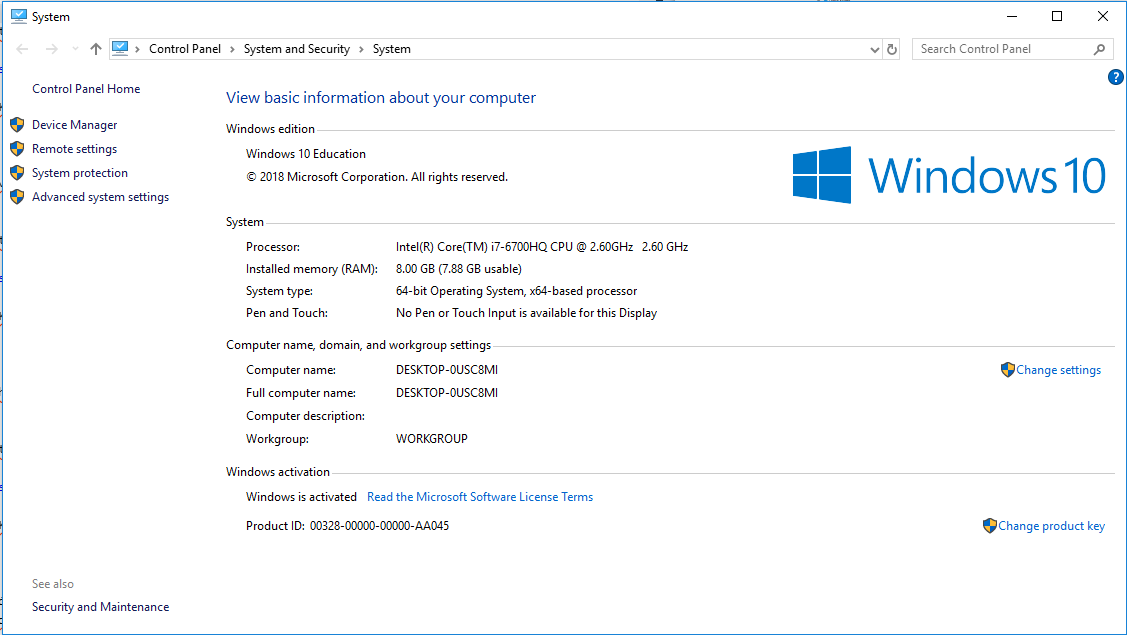
\includegraphics[scale=0.4]{image3/advanced}
    \end{center}
    \caption{Chọn Advanced System Settings.}
    \label{refhinh1}
    \end{figure}
\end{center}
\begin{center}
    \begin{figure}[htp]
    \begin{center}
     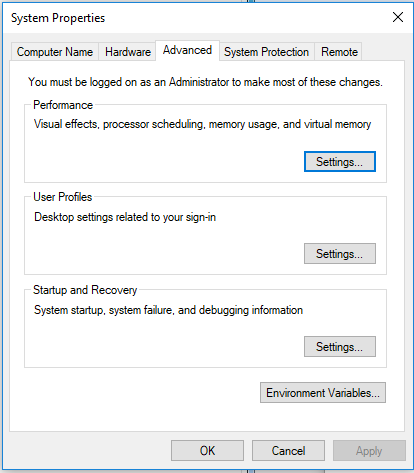
\includegraphics[scale=0.5]{image3/adv}
    \end{center}
    \caption{Chọn Advanced.}
    \label{refhinh1}
    \end{figure}
\end{center}
\newpage
    \item Nhấn New để tạo mới một biến môi trường có tên "JAVA\_HOME".
\begin{center}
    \begin{figure}[htp]
    \begin{center}
     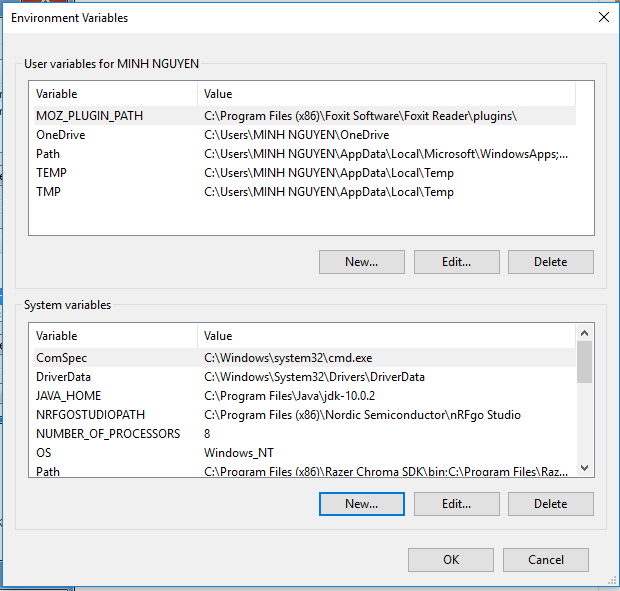
\includegraphics[scale=0.5]{image3/newjava}
    \end{center}
    \caption{Tạo một biến môi trường có tên "JAVA\_HOME".}
    \label{refhinh1}
    \end{figure}
\end{center}
\newpage
    \item Nhập vào đường dẫn tới thư mục JDK.\\
    Variable name: JAVA\_HOME\\
    Variable value: \textsf{C:/Program Files/Java/jdk-11.0.1}
\begin{center}
    \begin{figure}[htp]
    \begin{center}
     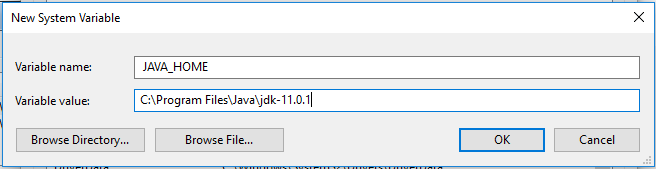
\includegraphics[scale=0.5]{image3/javahome}
    \end{center}
    \caption{Nhập Variable name và Variable value.}
    \label{refhinh1}
    \end{figure}
\end{center}
    \item Tiếp theo sửa đổi biến môi trường path\\
    Nhấn vào Edit, sau đó nhấn vào Edit text. Thêm vào phía trước giá trị của biến môi trường path:\textsf{\%JAVA\_HOME\%/bin;}
\begin{center}
    \begin{figure}[htp]
    \begin{center}
     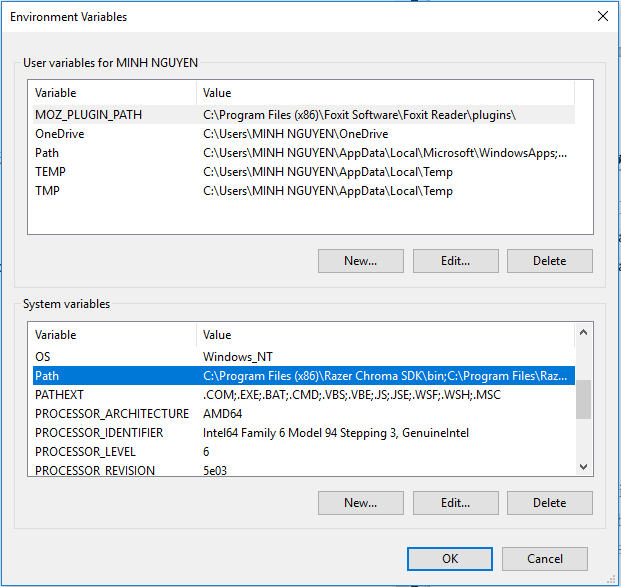
\includegraphics[scale=0.5]{image3/edit}
    \end{center}
    \caption{Nhấn vào Edit.}
    \label{refhinh1}
    \end{figure}
\end{center}
\newpage
\begin{center}
    \begin{figure}[htp]
    \begin{center}
     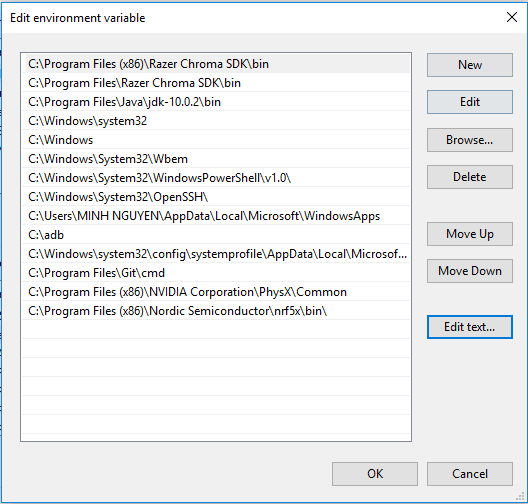
\includegraphics[scale=0.5]{image3/edittext}
    \end{center}
    \caption{Nhấn vào Edit text.}
    \label{refhinh1}
    \end{figure}
\end{center}
\begin{center}
    \begin{figure}[htp]
    \begin{center}
     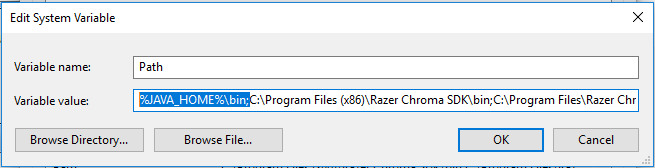
\includegraphics[scale=0.5]{image3/javaedit}
    \end{center}
    \caption{Hoàn tất thêm vào "\%JAVA\_HOME\%/bin".}
    \label{refhinh1}
    \end{figure}
\end{center}
 \end{enumerate}
 \subsection{Cài đặt Android Studio}
 Có nhiều công cụ để phát triển Android nhưng đến nay công cụ chính thức và mạnh mẽ nhất là Android Studio. Đây là IDE (Môi trường phát triển tích hợp) chính thức cho nền tảng Android, được phát triển bởi Google và được sử dụng để tạo phần lớn các ứng dụng mà bạn có thể sử dụng hàng ngày.
 
 Android Studio lần đầu tiên được công bố tại hội nghị Google I/O vào năm 2013 và được phát hành cho công chúng vào năm 2014 sau nhiều phiên bản beta khác nhau. Trước khi được phát hành, các nhà phát triển Android thường sử dụng các công cụ như Eclipse IDE, một IDE Java chung cũng hỗ trợ nhiều ngôn ngữ lập trình khác.
 
 Android Studio khiến việc tạo ứng dụng trở nên dễ dàng hơn đáng kể so với phần mềm không chuyên dụng. Đối với người mới bắt đầu, có rất nhiều thứ để học và nhiều thông tin có sẵn, thậm chí thông qua các kênh chính thức nhưng chúng có thể đã lỗi thời hoặc quá nhiều thông tin khiến họ cảm thấy choáng ngợp.
 
 Chức năng của Android Studio là cung cấp giao diện để tạo các ứng dụng và xử lý phần lớn các công cụ quản lý file phức tạp đằng sau hậu trường. Ngôn ngữ lập trình được sử dụng ở đây là Java và được cài đặt riêng trên thiết bị của bạn. Android Studio rất đơn giản, bạn chỉ cần viết, chỉnh sửa và lưu các dự án của mình và các file trong dự án đó. Đồng thời, Android Studio sẽ cấp quyền truy cập vào Android SDK.
 
 Hãy coi đây là đuôi cho code Java cho phép nó chạy trơn tru trên các thiết bị Android và tận dụng lợi thế của phần cứng gốc. Bạn cần sử dụng ngôn ngữ lập trình Java để viết các chương trình, Android SDK có nhiệm vụ kết nối các phần này lại với nhau. Cùng lúc đó Android Studio kích hoạt để chạy code, thông qua trình giả lập hoặc qua một phần cứng kết nối với thiết bị. Sau đó, bạn cũng có thể “gỡ rối” chương trình khi nó chạy và nhận phản hồi giải thích sự cố, v.v… để bạn có thể nhanh chóng giải quyết vấn đề.
 
 Google đã nỗ lực rất nhiều để làm cho Android Studio trở nên mạnh mẽ và hữu ích nhất có thể. Nó cung cấp những gợi ý trực tiếp trong khi viết code và thường đề xuất những thay đổi cần thiết để sửa lỗi hoặc làm code hiệu quả hơn. Ví dụ, nếu không sử dụng biến, biến đó sẽ được tô đậm bằng màu xám. Và khi bắt đầu gõ một dòng code, Android Studio sẽ cung cấp danh sách gợi ý tự hoàn thành để giúp bạn hoàn thiện dòng code đó. Chức năng này rất hữu ích khi bạn không nhớ được chính xác cú pháp hoặc để tiết kiệm thời gian\cite{tl3}.
 
 Hướng dẫn cài đặt android stuido.
 \begin{enumerate}
     \item Vào trang web \url{https://developer.android.com/studio/} để download android studio.
\newpage
\begin{center}
    \begin{figure}[htp]
    \begin{center}
     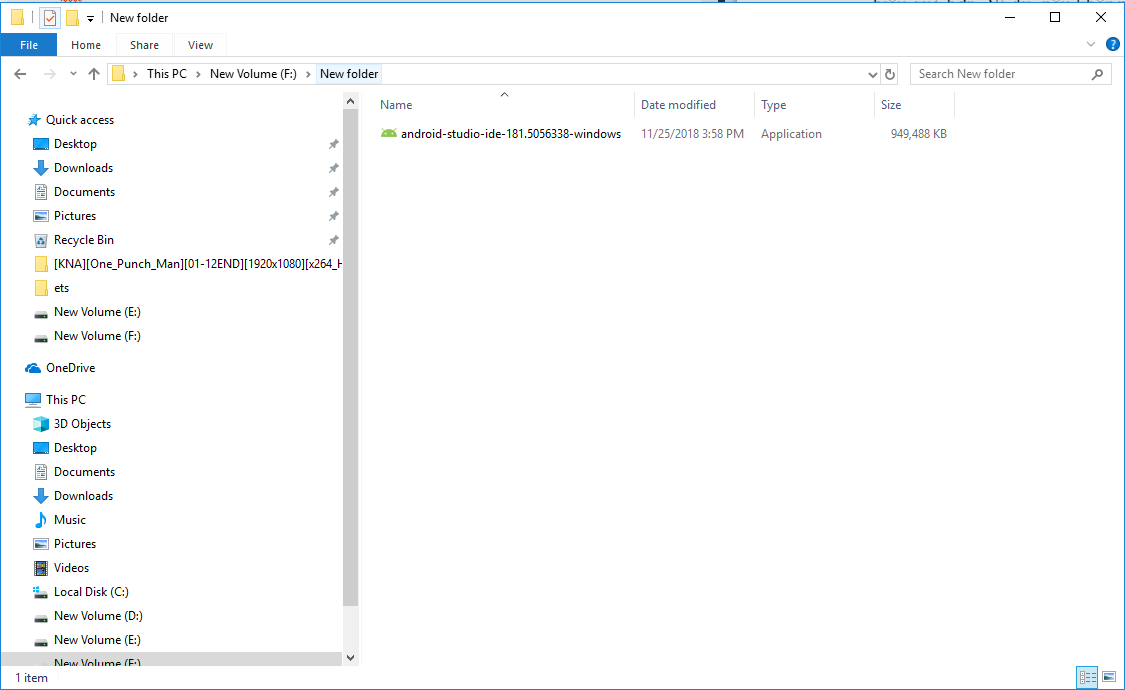
\includegraphics[scale=0.45]{image3/androidstudio}
    \end{center}
    \caption{File android studio.}
    \label{refhinh1}
    \end{figure}
\end{center}
    \item Chạy file android studio tải về 
\begin{center}
    \begin{figure}[htp]
    \begin{center}
     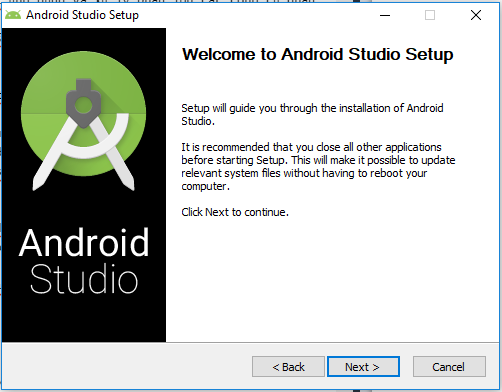
\includegraphics[scale=0.6]{image3/caidat1}
    \end{center}
    \caption{Nhấn Next để cài đặt.}
    \label{refhinh1}
    \end{figure}
\end{center}
\newpage
\begin{center}
    \begin{figure}[htp]
    \begin{center}
     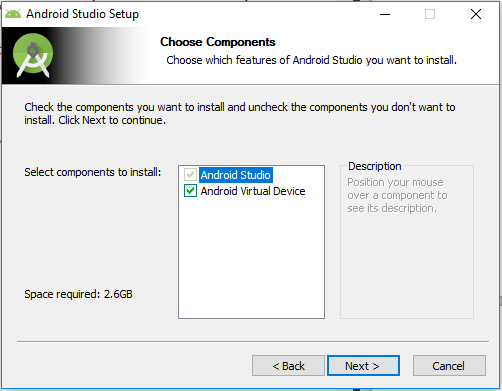
\includegraphics[scale=0.6]{image3/caidat2}
    \end{center}
    \caption{Nhấn Next để cài đặt.}
    \label{refhinh1}
    \end{figure}
\end{center}

\begin{center}
    \begin{figure}[htp]
    \begin{center}
     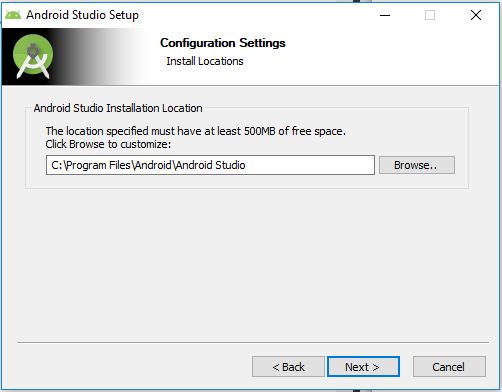
\includegraphics[scale=0.6]{image3/caidat3}
    \end{center}
    \caption{Chọn ví trí lưu, nhấn Next để cài đặt.}
    \label{refhinh1}
    \end{figure}
\end{center}
\newpage
\begin{center}
    \begin{figure}[htp]
    \begin{center}
     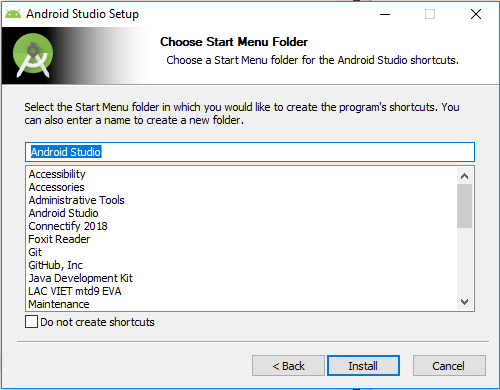
\includegraphics[scale=0.6]{image3/caidat4}
    \end{center}
    \caption{Nhấn Install để cài đặt.}
    \label{refhinh1}
    \end{figure}
\end{center}

\begin{center}
    \begin{figure}[htp]
    \begin{center}
     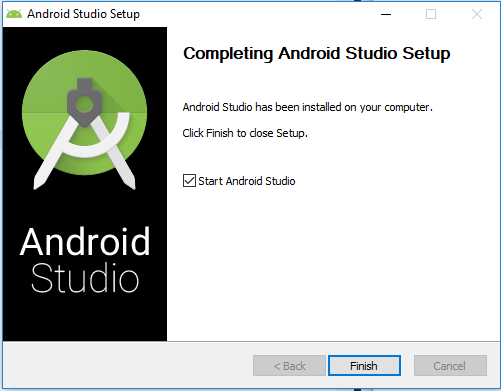
\includegraphics[scale=0.6]{image3/caidat5}
    \end{center}
    \caption{Nhấn Finish để cài đặt.}
    \label{refhinh1}
    \end{figure}
\end{center}
 \end{enumerate}
 
\newpage
\subsection{Cài đặt hệ điều hành Android Things}
Để cài hệ điều hành Android Things, cần thực hiện theo 3 bước sau.\\
Bước 1: Tạo Image Boot cho hệ điều hành Android Things.
\begin{enumerate}
\item Vào trang \url{https://partner.android.com/things/console/}, đăng nhập với tài khoản của Google. Nên sử dụng trình duyệt \href{https://www.google.com/chrome/}{Google Chrome} để tránh trường hơp không vào được trang
\begin{center}
\begin{figure}[htp]
\begin{center}
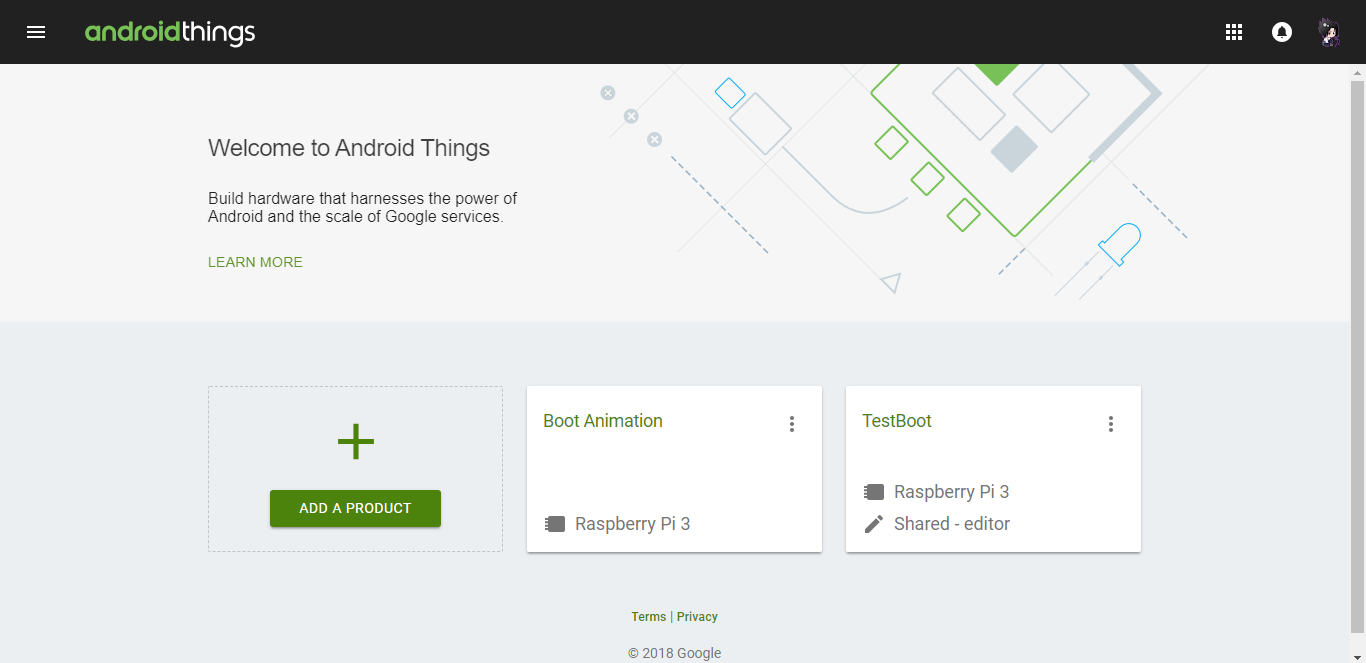
\includegraphics[scale=0.4]{image3/sat1.png}
\end{center}
\caption{Màn hình giao diện - tạo Image Boot.}
\label{refhinh1}
\end{figure}
\end{center}
\item Nhấn vào "ADD A PRODUCT" hoặc biểu tượng dấu cộng "+".
\begin{center}
\begin{figure}[htp]
\begin{center}
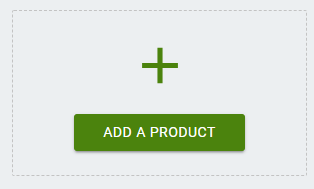
\includegraphics[scale=1]{image3/sat2.png}
\end{center}
\caption{Nhấn + để tạo PRODUCT mới.}
\label{refhinh1}
\end{figure}
\end{center}
\item Bảng "Create new product" hiện lên. Điền thông tin vào các trường: 
\begin{center}
\begin{figure}[htp]
\begin{center}
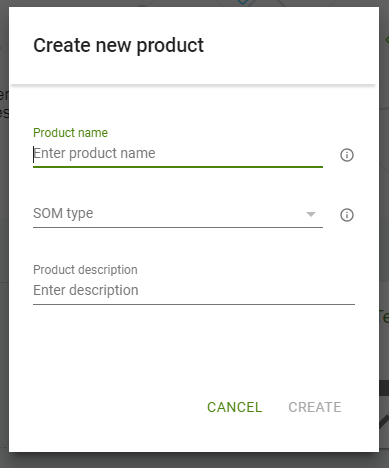
\includegraphics[scale=0.8]{image3/sat3.png}
\end{center}
\caption{Thêm thông tin PRODUCT vào bảng.}
\label{refhinh1}
\end{figure}
\end{center}
\begin{itemize}
\item "Product name" - là tên sản phẩm mà mình sẽ làm việc, yêu cầu có ít nhất một ký tự chữ, ví dụ "Starter".
\item "SOM type" - là mạch phần cứng được sử dụng, ở đây dùng Rpi3 nên chọn "Raspberry Pi 3".
\item "Product description" là mô tả về sản phẩm, trường này không bắt buộc phải điền 
\end{itemize}
\item Sau khi điền xong, nhấn "Create" để tạo sản phẩm.
\begin{center}
\begin{figure}[htp]
\begin{center}
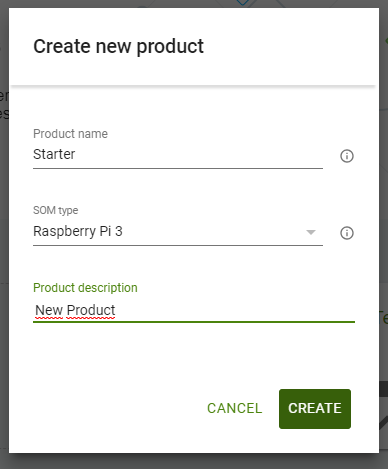
\includegraphics[scale=0.6]{image3/sat4.png}
\end{center}
\caption{Nhấn CREATE để tạo sản phẩm.}
\label{refhinh1}
\end{figure}
\end{center}
\newpage
\item Sau khi tạo xong, màn hình sẽ hiện ra kết quả khi tạo thành công, ấn vô ô ("ei3ri4" - theo ví dụ) ở phần "Models".
\begin{center}
\begin{figure}[htp]
\begin{center}
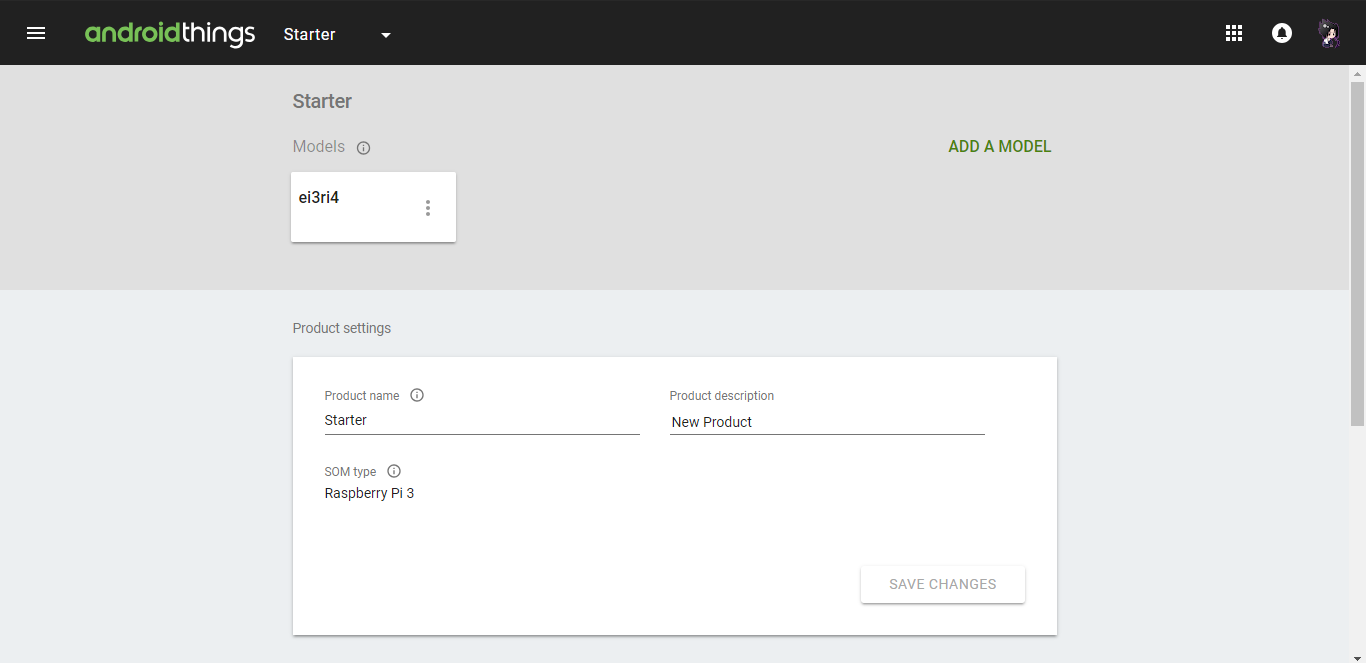
\includegraphics[scale=0.4]{image3/sat5.png}
\end{center}
\caption{Tạo thành công sản phẩm.}
\label{refhinh1}
\end{figure}
\end{center}
\item Tại tab "BUILD", ấn vào nút "NEW" ở gần bên phải giữa màn hình để tạo mới một Image Boot.
\begin{center}
\begin{figure}[!htp]
\begin{center}
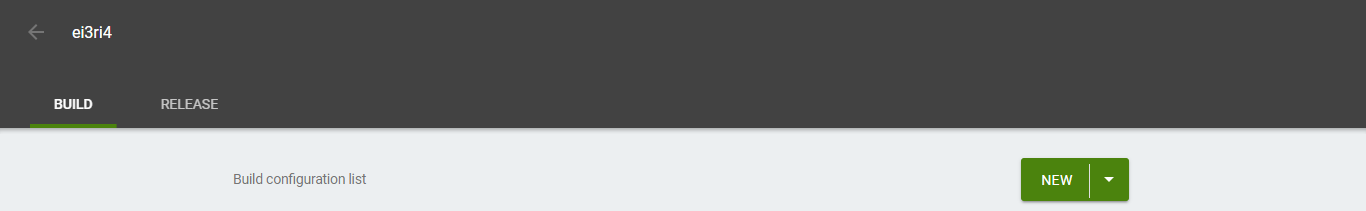
\includegraphics[scale=0.4]{image3/sat6.png}
\end{center}
\caption{Ấn NEW để tạo mới Image Boot.}
\label{refhinh1}
\end{figure}
\end{center}
\newpage
\item Tại khung xổ xuống, chọn "Start from scratch".
\begin{center}
\begin{figure}[htp]
\begin{center}
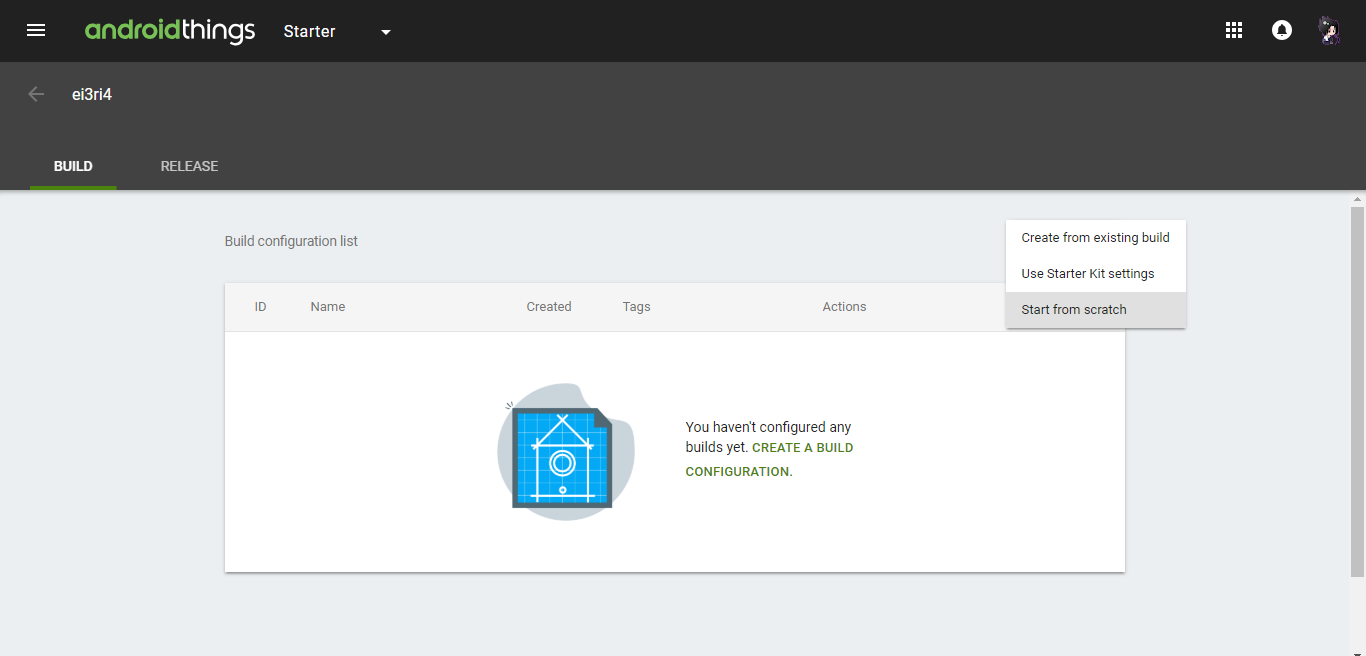
\includegraphics[scale=0.38]{image3/sat7.png}
\end{center}
\caption{Chọn Start from scratch.}
\label{refhinh1}
\end{figure}
\end{center}
\item Tại trường "1", nhập tên Image Boot muốn tạo, ví dụ "New Build". Sau đó ấn "NEXT".
\begin{center}
\begin{figure}[htp]
\begin{center}
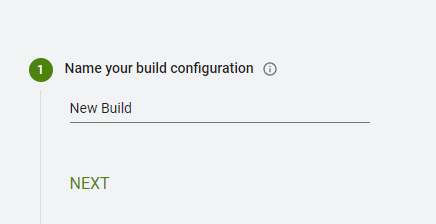
\includegraphics[scale=0.65]{image3/sat8.png}
\end{center}
\caption{Nhập tên Image Boot.}
\label{refhinh1}
\end{figure}
\end{center}
\item Tại trường "2", chọn phiên bản Android Things mới nhất, thường có chữ "(latest)" ở cột "OS version". Sau đó ấn "NEXT".
\begin{center}
\begin{figure}[htp]
\begin{center}
\includegraphics[scale=0.6]{image3/sat9.png}
\end{center}
\caption{Chọn phiên bản Android Things mới nhất.}
\label{refhinh1}
\end{figure}
\end{center}
\item Trường "3" là nơi để upload ứng dụng được chạy tự động đầu tiên sau khi hệ điều hành được khởi động. Nếu muốn thiết lập cho ứng dụng tự khởi chạy thì ấn chọn "SELECT APPS". Nhưng vẫn khuyên không nên chọn và ấn "NEXT".
\begin{center}
\begin{figure}[htp]
\begin{center}
\includegraphics[scale=0.5]{image3/sat10.png}
\end{center}
\caption{Chọn NEXT tại bước này.}
\label{refhinh1}
\end{figure}
\end{center}
\item \label{truong4} Trường "4" sẽ là nơi để cài đặt hình ảnh load đầu tiên khi hệ điều hành được khởi động. Có thể thay đổi hình ảnh này, điều này sẽ được hướng dẫn thêm ở \hyperref[bootanimation]{mục \ref*{bootanimation}}. Sau đó ấn "NEXT".
\begin{center}
\begin{figure}[htp]
\begin{center}
\includegraphics[scale=0.45]{image3/sat11.png}
\end{center}
\caption{Chọn NEXT tại bước này -  \hyperref[bootanimation]{Xem thêm \ref*{bootanimation}}.}
\label{refhinh1}
\end{figure}
\end{center}
\item \label{truong5} Trường "5" là phần chỉnh sửa thông tin về chân cắm của phần cứng. KHÔNG NÊN CAN THIỆP VÀO PHẦN NÀY, chỉ nên can thiệp nếu đã đủ khả năng làm việc với mạch. Sau đó ấn "NEXT".
\begin{center}
\begin{figure}[htp]
\begin{center}
\includegraphics[scale=0.5]{image3/sat12.png}
\end{center}
\caption{Chọn NEXT tại bước này.}
\label{refhinh1}
\end{figure}
\end{center}
\item Tại trường "6" sẽ thống kê lại những thiết lập đã chọn. Ấn "CREATE BUILD" để tạo Image Boot.
\begin{center}
\begin{figure}[htp]
\begin{center}
\includegraphics[scale=0.6]{image3/sat13.png}
\end{center}
\caption{Thông tin về bản Image Boot.}
\label{refhinh1}
\end{figure}
\end{center}
\newpage
\item Vậy là đã tạo xong một bản Image Boot rồi.
\begin{center}
\begin{figure}[htp]
\begin{center}
\includegraphics[scale=0.45]{image3/sat14.png}
\end{center}
\caption{Ấn CREATE BUILD để tạo.}
\label{refhinh1}
\end{figure}
\end{center}
\item Để tải bản Image Boot, tại cột "Actions", ấn vô "Download".
\begin{center}
\begin{figure}[htp]
\begin{center}
\includegraphics[scale=0.52]{image3/sat17.png}
\end{center}
\caption{Ấn Download tại bản Image Boot muốn tải.}
\label{refhinh1}
\end{figure}
\end{center}
\newpage
\item Tiếp tục ấn vô "Development" để thực hiện quá trình tải.
\begin{center}
\begin{figure}[htp]
\begin{center}
\includegraphics[scale=0.7]{image3/sat18.png}
\end{center}
\caption{Chọn Development.}
\label{refhinh1}
\end{figure}
\end{center}
\item Đợi từ 5 đến 10 phút là tải xong (tùy thuộc vào tốc độ mạng).
\begin{center}
\begin{figure}[htp]
\begin{center}
\includegraphics[scale=0.6]{image3/sat19.png}
\end{center}
\caption{Chờ để tải xuống.}
\label{refhinh1}
\end{figure}
\end{center}
\item File Image Boot đã tải xong, dung lượng tầm khoảng 300 - 350 (MB), định dạng file là ".zip".
\begin{center}
\begin{figure}[htp]
\begin{center}
\includegraphics[scale=0.75]{image3/sat20.png}
\end{center}
\caption{Đã tải thành công.}
\label{refhinh1}
\end{figure}
\end{center}
\end{enumerate}
Bước 2: Cài đặt hệ điều hành lên thẻ nhớ (dung lượng từ 8GB trở lên).\\
\hspace*{0.25cm}Cách 1: Sử dụng phần mềm \href{https://www.sdcard.org/downloads/formatter_4/}{SD Card Formatter}, \href{https://sourceforge.net/projects/win32diskimager/}{Win32 Disk Image}.
\newpage
\begin{enumerate}
\item Cắm thẻ nhớ MicroSD vào đầu đọc thẻ, sau đó cắm vào máy tính. Sẽ hiện ra thông báo yêu cầu định dạng lại thẻ nhớ, nhấn "Cancel".
\begin{center}
\begin{figure}[htp]
\begin{center}
 \includegraphics[scale=0.8]{image3/buoc2cach1s1.png}
\end{center}
\caption{Nhấn Cancel sau khi cắm thẻ nhớ vô máy.}
\label{refhinh1}
\end{figure}
\end{center}
\item Chạy phần mềm SD Card Formatter để định dạng thẻ nhớ. Lưu ý, phải chọn đứng ổ đĩa của thẻ nhớ để tránh trường hợp định dạng nhầm ổ cứng máy tính. Ấn "Refresh" để tự động tìm thẻ nhớ đã được kết nối.
\begin{center}
\begin{figure}[htp]
\begin{center}
\includegraphics[scale=0.75]{image3/buoc2cach1s2.png}
\end{center}
\caption{Nhấn Refresh để tự động tìm thẻ nhớ.}
\label{sdcardformat}
\end{figure}
\end{center}
\item Sau khi tìm được, chọn thẻ nhớ dùng để cài hệ điều hành. Nhấn "Format" để định dạng.
\begin{center}
\begin{figure}[htp]
\begin{center}
\includegraphics[scale=0.7]{image3/buoc2cach1s3.png}
\end{center}
\caption{Nhấn Format để định dạng.}
\label{refhinh1}
\end{figure}
\end{center}
\item Thông báo nhắc nhở sẽ hiện lên, nhấn "Yes" để thực hiện quá trình định dạng thẻ nhớ.
\begin{center}
\begin{figure}[htp]
\begin{center}
 \includegraphics[scale=0.65]{image3/buoc2cach1s4.png}
\end{center}
\caption{Nhấn Yes.}
\label{refhinh1}
\end{figure}
\end{center}
\item Định dạng xong, phần mềm sẽ hiển thị như  \hyperref[finishformat]{hình \ref*{finishformat}}. Nhấn "OK" và thoát.
\begin{center}
\begin{figure}[htp]
\begin{center}
\includegraphics[scale=0.7]{image3/buoc2cach1s5.png}
\end{center}
\caption{Nhấn OK.}
\label{finishformat}
\end{figure}
\end{center}
\item Giải nén tập tin Image Boot vừa tải xong. Sau khi giải nén xong sẽ có một tập tin "iot\_rpi3.img".
\begin{center}
\begin{figure}[htp]
\begin{center}
\includegraphics[scale=0.6]{image3/buoc2cach1s6.png}
\end{center}
\caption{Giải nén tập tin Image Boot vừa tải.}
\label{refhinh1}
\begin{center}
\includegraphics[scale=0.73]{image3/buoc2cach1s7.png}
\end{center}
\caption{Nhận được tập tin "iot\_rpi3.img".}
\label{refhinh1}
\end{figure}
\end{center}
\item Chạy phần mềm Win32 Disk Image để cài hệ điều hành lên thẻ nhớ.
\begin{center}
\begin{figure}[htp]
\begin{center}
\includegraphics[scale=0.65]{image3/buoc2cach1s8.png}
\end{center}
\caption{Chạy phần mềm Win32 Disk Image.}
\label{refhinh1}
\end{figure}
\end{center}
\newpage
\item Chọn đường dẫn tới tập tin "iot\_rpi3.img" vừa được giải nén xong. Ví dụ: \textsf{C:/Download/}
\begin{center}
\begin{figure}[htp]
\begin{center}
\includegraphics[scale=0.6]{image3/buoc2cach1s9.png}
\end{center}
\caption{Chọn đường dẫn tới tập tin Image Boot đã được giải nén.}
\label{refhinh1}
\end{figure}
\end{center}
\newpage
\item Chọn thẻ nhớ đã được định dạng.
\begin{center}
\begin{figure}[htp]
\begin{center}
\includegraphics[scale=0.65]{image3/buoc2cach1s10.png}
\end{center}
\caption{Chọn thẻ nhớ.}
\label{refhinh1}
\end{figure}
\end{center}
\item Ấn "Write" để ghi hệ điều hành Android Things vào thẻ nhớ.
\begin{center}
\begin{figure}[htp]
\begin{center}
\includegraphics[scale=0.67]{image3/buoc2cach1s11.png}
\end{center}
\caption{Chọn thẻ nhớ.}
\label{refhinh1}
\end{figure}
\end{center}
\item Chương trình sẽ hiện ra tin nhắn cảnh báo, ấn "Yes" để tiếp tục quá trình.
\begin{center}
\begin{figure}[htp]
\begin{center}
\includegraphics[scale=0.65]{image3/buoc2cach1s12.png}
\end{center}
\caption{Nhấn Yes để tiếp tục.}
\label{refhinh1}
\end{figure}
\end{center}
\newpage
\item Đợi từ 2 - 5 phút (tùy vào máy tính).
\begin{center}
\begin{figure}[htp]
\begin{center}
\includegraphics[scale=0.65]{image3/buoc2cach1s13.png}
\end{center}
\caption{Chờ đợi quá trình ghi hệ đièu hành.}
\label{refhinh1}
\end{figure}
\end{center}
\item Sau khi thực hiện quá trình ghi xong, máy tính sẽ hiển thị thông báo yêu cầu định dạng lại thẻ nhớ, ấn "Cancel" để thoát nhé.
\begin{center}
\begin{figure}[htp]
\begin{center}
\includegraphics[scale=0.65]{image3/buoc2cach1s14.png}
\end{center}
\caption{Nhấn Cancel.}
\label{refhinh1}
\end{figure}
\end{center}
\newpage
\item Thông báo của việc ghi hệ điều hành lên thẻ nhớ được thực hiện thành công, nhấn "OK".
\begin{center}
\begin{figure}[htp]
\begin{center}
\includegraphics[scale=0.65]{image3/buoc2cach1s15.png}
\end{center}
\caption{Nhấn OK để tắt thông báo.}
\label{refhinh1}
\end{figure}
\end{center}
\item Vậy là đã cài đặt xong hệ điều hành Android Things lên thẻ nhớ. Việc tiếp theo là gắn thẻ nhớ vào mạch Rpi3.
\begin{center}
\begin{figure}[htp]
\begin{center}
\includegraphics[scale=0.65]{image3/buoc2cach1s16.png}
\end{center}
\caption{Nhấn Exit để thoát chương trình.}
\label{refhinh1}
\end{figure}
\end{center}
\end{enumerate}
\newpage
\hspace*{0.25cm}Cách 2: sử dụng phần mềm \href{https://partner.android.com/things/console/#/tools}{android-things-setup-utility}.
\begin{enumerate}
\item Cắm thẻ nhớ MicroSD vào đầu đọc thẻ, sau đó cắm vào máy tính.
\begin{center}
\begin{figure}[htp]
\begin{center}
\includegraphics[scale=0.8]{image3/buoc2cach1s1.png}
\end{center}
\caption{Nhấn Cancel sau khi cắm thẻ nhớ vô máy.}
\label{refhinh1}
\end{figure}
\end{center}
\item Tải phần mềm từ trang \url{https://partner.android.com/things/console/#/tools}.
\begin{center}
\begin{figure}[htp]
\begin{center}
\includegraphics[scale=0.27]{image3/buoc2cach2s2.png}
\end{center}
\caption{Nhấn DOWNLOAD để tải phần mềm.}
\label{refhinh1}
\end{figure}
\end{center}
\newpage
\item Giải nén phần mềm vừa tải được, chọn tập tin tương ứng với hệ điều hành mà máy tính đang sử dụng.
\begin{center}
\begin{figure}[htp]
\begin{center}
\includegraphics[scale=0.67]{image3/buoc2cach2s3.png}
\end{center}
\caption{Giải nén phần mềm.}
\label{refhinh1}
\end{figure}
\end{center}
\item Chạy tập tin "android-things-setup-utility-windows.exe" (đối với Windows) bằng quyền Administrator. Ấn "YES" nếu có hiện thông báo.
\begin{center}
\begin{figure}[htp]
\begin{center}
\includegraphics[scale=0.57]{image3/buoc2cach2s4.png}
\end{center}
\caption{Chuột phải, chọn Run as administrator.}
\label{refhinh1}
\end{figure}
\end{center}
\item Chọn "1" để tiến hành cài đặt hệ điều hành Android Things.
\begin{center}
\begin{figure}[htp]
\begin{center}
\includegraphics[scale=0.55]{image3/buoc2cach2s5.png}
\end{center}
\caption{Nhấn 1.}
\label{refhinh1}
\end{figure}
\end{center}
\item Chọn "1" để chọn thiết bị phần cứng, ở đây là "Raspberry Pi 3".
\begin{center}
\begin{figure}[htp]
\begin{center}
\includegraphics[scale=0.55]{image3/buoc2cach2s6.png}
\end{center}
\caption{Nhấn 1 để tiếp tục.}
\label{refhinh1}
\end{figure}
\end{center}
\item Sau vài giây để chương trình tiến hành tải công cụ hỗ trợ. Tại đây, có sự 2 lựa chọn phiên bản hệ điều hành để ghi lên thẻ nhớ.
\begin{center}
\begin{figure}[htp]
\begin{center}
\includegraphics[scale=0.55]{image3/buoc2cach2s7.png}
\end{center}
\caption{Lựa chọn phiên bản để ghi.}
\label{refhinh1}
\end{figure}
\end{center}
\begin{itemize}
\item Nếu chưa tạo bản Image Boot và muốn sử dụng bản mặc định thì ấn "1". Đợi từ 10 - 15 phút để tải bản Image Boot.
\begin{center}
\begin{figure}[htp]
\begin{center}
\includegraphics[scale=0.55]{image3/buoc2cach2s8a.png}
\end{center}
\caption{Nhấn 1 nếu cài bản mặc định.}
\label{refhinh1}
\end{figure}
\end{center}
\item Nếu đã tạo (Bước 1) thì ấn "2" để chọn đường dẫn tới tập tin ".zip". Dán địa chỉ của tập tin ".zip" và ấn ENTER.
\begin{center}
\begin{figure}[htp]
\begin{center}
\includegraphics[scale=0.5]{image3/buoc2cach2s8b.png}
\end{center}
\caption{Nhấn 2 để cài bản đã tải tại Bước 1.}
\label{refhinh1}
\end{figure}
\end{center}
\item Dán địa chỉ của tập tin ".zip" và ấn ENTER. Ở đây, địa chỉ là: \textsf{C:/Users/phuon/Downloads/Starter\_Raspberry Pi 3\_1\_New-
Build\_development\_build.zip} rồi ấn "ENTER".
\begin{center}
\begin{figure}[htp]
\begin{center}
\includegraphics[scale=0.5]{image3/buoc2cach2s8c.png}
\end{center}
\caption{Dán địa chỉ chứa tập tin Image Boot .zip.}
\label{refhinh1}
\end{figure}
\end{center}
\end{itemize}
\newpage
\item Sau tải xong công cụ Etcher-cli, ấn ENTER để nhận thẻ nhớ.
\begin{center}
\begin{figure}[htp]
\begin{center}
\includegraphics[scale=0.5]{image3/buoc2cach2s9.png}
\end{center}
\caption{Nhấn ENTER để chọn thẻ nhớ.}
\label{refhinh1}
\end{figure}
\end{center}
\item Nhấn phím mũi tên để chọn thẻ nhớ cần ghi hệ điều hành. Nhấn "ENTER" để xác nhận thẻ nhớ.
\begin{center}
\begin{figure}[htp]
\begin{center}
\includegraphics[scale=0.53]{image3/buoc2cach2s10.png}
\end{center}
\caption{Chọn thẻ nhớ rồi nhấn ENTER.}
\label{refhinh1}
\end{figure}
\end{center}
\newpage
\item Nhấn "y", rồi nhấn "ENTER" để tiếp tục. \textit{Lưu ý, sau khi cài đặt xong sẽ xuất hiện thông báo yêu cầu định dạng lại thẻ nhớ của Windows, ấn "Cancel" nhé!}
\begin{center}
\begin{figure}[htp]
\begin{center}
\includegraphics[scale=0.52]{image3/buoc2cach2s11.png}
\end{center}
\caption{Nhấn y, rồi nhấn ENTER.}
\label{refhinh1}
\end{figure}
\end{center}
\item Đợi khoảng 5 phút thì cài đặt xong. Sau đó ấn "n" để thoát thiết lập mạng.
\begin{center}
\begin{figure}[htp]
\begin{center}
\includegraphics[scale=0.52]{image3/buoc2cach2s12.png}
\end{center}
\caption{Nhấn n rồi nhấn ENTER.}
\label{refhinh1}
\end{figure}
\end{center}
\item Ấn Enter để thoát chương trình.
\begin{center}
\begin{figure}[htp]
\begin{center}
\includegraphics[scale=0.53]{image3/buoc2cach2s13.png}
\end{center}
\caption{Nhấn ENTER để thoát.}
\label{refhinh1}
\end{figure}
\end{center}
\end{enumerate}
\textit{\hspace*{0.25cm}Lưu ý: Sau khi cài hệ điều hành xong, gắn thẻ nhớ vào Rpi3, rồi mới được cắm nguồn. Tuy nhiên nếu có kết nối màn hình HDMI thì nên cắm cáp HDMI trước rồi mới cắm nguồn để tránh trường hợp hình ảnh hiển thị bị sai độ phân giải.}\\

Bước 3: Kết nối mạng cho Raspberry Pi 3 để lấy địa chỉ IP.\\
\hspace*{0.25cm}Cách 1: Kết nối wifi và có màn hình. 
\begin{enumerate}
\item Cắm cáp HDMI với màn hình, gắn bàn phím và chuột vào để điều khiển (nếu màn hình cảm ứng thì không cần thực hiện bước này). Sau đó cắm nguồn cho Rpi3.
\begin{center}
\begin{figure}[htp]
\begin{center}
\includegraphics[scale=0.065]{image3/buoc3s1.JPG}
\end{center}
\caption{Cắm các kết nối trước rồi mới cắm nguồn.}
\label{refhinh1}
\end{figure}
\end{center}
\item Đợi từ 2 - 5 phút cho lần khởi chạy ban đầu, các lần khởi chạy tiếp theo thì thời gian sẽ nhanh hơn.
\begin{center}
\begin{figure}[htp]
\begin{center}
\includegraphics[scale=0.075]{image3/buoc3s2.JPG}
\end{center}
\caption{Chờ hệ điều hành khởi động.}
\label{refhinh1}
\end{figure}
\end{center}
\newpage
\item Tại màn hình chính của Android Things, kéo chuột và nhấp vào phần "Networks".
\begin{center}
\begin{figure}[htp]
\begin{center}
\includegraphics[scale=0.1]{image3/buoc3s3.JPG}
\end{center}
\caption{Chọn Networks.}
\label{refhinh1}
\end{figure}
\end{center}
\item Chọn phần Wi-Fi để kết nối với mạng wifi.
\begin{center}
\begin{figure}[htp]
\begin{center}
\includegraphics[scale=0.15]{image3/buoc3s4.JPG}
\end{center}
\caption{Chọn Wi-Fi.}
\label{refhinh1}
\end{figure}
\end{center}
\item Nếu mới lần đầu kết nối, thì sẽ hiện chữ "Off". Để bật wifi, ấn vào nút cùng hàng với "Off" ở phía bên phải màn hình.
\begin{center}
\begin{figure}[htp]
\begin{center}
\includegraphics[scale=0.12]{image3/buoc3s5.JPG}
\end{center}
\caption{Ấn nút bên phải để bật wifi.}
\label{refhinh1}
\end{figure}
\end{center}
\newpage
\item Sau khi bật wifi, danh sách các wifi khả dụng sẽ được hiện ra.
\begin{center}
\begin{figure}[htp]
\begin{center}
\includegraphics[scale=0.12]{image3/buoc3s6.JPG}
\end{center}
\caption{Danh sách wifi khả dụng.}
\label{refhinh1}
\end{figure}
\end{center}
\item Chọn wifi, và nhập vào mật khẩu của wifi mà muốn thiết bị kết nối. Nhấn "CONNECT".
\begin{center}
\begin{figure}[htp]
\begin{center}
\includegraphics[scale=0.12]{image3/buoc3s7.JPG}
\end{center}
\caption{Nhập mật khẩu và nhấn CONNECT.}
\label{refhinh1}
\end{figure}
\end{center}
\item Nếu thấy hiện chữ "Connected", tức là đã kết nối wifi thành công. Ấn dấu mũi tên \b{<} để quay lại màn hình chính, địa chỉ của thiết bị sẽ được hiện ra. Ở đây là: "192.168.2.55".
\begin{center}
\begin{figure}[htp]
\begin{center}
\includegraphics[scale=0.15]{image3/buoc3s8.JPG}
\end{center}
\caption{Nhấn < để về màn hình chính.}
\label{refhinh1}
\end{figure}
\end{center}
\newpage
\item Địa chỉ IP của thiết bị sẽ được hiện ra trong phần "Networks". Ở đây là: "192.168.2.55".
\begin{center}
\begin{figure}[htp]
\begin{center}
\includegraphics[scale=0.17]{image3/buoc3s9.JPG}
\end{center}
\caption{Networks hiển thị IP của mạch Rpi3.}
\label{refhinh1}
\end{figure}
\end{center}
\end{enumerate}
\hspace*{0.25cm}Cách 2: Kết nối mạng dây và không có màn hình. 
\begin{enumerate}
\item Cắm cáp Ethernet vào mạch Rpi3, sau đó cắm nguồn.
\begin{center}
\begin{figure}[htp]
\begin{center}
\includegraphics[scale=0.08]{image3/buoc3s10.JPG}
\end{center}
\caption{Cắm dây Ethernet và cắm nguồn.}
\label{refhinh1}
\end{figure}
\end{center}
\item Đợi từ 2 - 5 phút cho lần khởi chạy ban đầu, các lần khởi chạy tiếp theo thì thời gian sẽ nhanh hơn.
\item Kết nối laptop/desktop cùng với mạng đã kết nối với Rpi3. Sử dụng phần mềm \hyperref[scanip]{Advanced IP Scanner}, tìm với tên tại cột "Nhà sản xuất" là "Raspberry Pi Fundation" để lấy địa chỉ IP (192.168.2.55).
\begin{center}
\begin{figure}[htp]
\begin{center}
\includegraphics[scale=0.65]{image3/buoc3s11.png}
\end{center}
\caption{Chạy chương trình \hyperref[scanip]{Advanced IP Scanner} để quét địa chỉ IP của Rpi3.}
\label{refhinh1}
\end{figure}
\end{center}
\end{enumerate}
Bước 4: Kết nối với Raspberry Pi 3 bằng địa chỉ IP.
\begin{enumerate}
\item Sau khi có được địa chỉ của mạch Rpi3. Chạy ứng dụng \hyperref[ADB]{ADB} để thực hiện việc kết nối.
\begin{center}
\begin{figure}[htp]
\begin{center}
\includegraphics[scale=0.62]{image3/buoc3s12.png}
\end{center}
\caption{Truy cập thư mục platform-tools.}
\end{figure}
\end{center}
\item Chạy "Command Prompt" (Windows) hoặc "Terminal" (Mac/Linux), tại thư mục (platform-tools) chứa tập tin "adb".
\begin{center}
\begin{figure}[htp]
\begin{center}
\includegraphics[scale=0.6]{image3/buoc3s13.png}
\end{center}
\caption{Chạy Command Prompt tại thư mục platform-tools.}
\end{figure}
\end{center}
\item Nhập lệnh "adb connect <IP>", với <IP> là địa chỉ IP của mạch Rpi3. Ví dụ "adv connect 192.68.2.55".
\begin{center}
\begin{figure}[htp]
\begin{center}
\includegraphics[scale=0.55]{image3/buoc3s14.png}
\end{center}
\caption{Kết nối với thiết bị "adb connect <IP>".}
\label{refhinh1}
\end{figure}
\end{center}
\newpage
\item Kết nối thành công với địa chỉ IP 192.168.2.55 thông qua port 5555.
\begin{center}
\begin{figure}[htp]
\begin{center}
\includegraphics[scale=0.65]{image3/buoc3s15.png}
\end{center}
\caption{Kết nối với mạch Raspberry Pi 3 thành công.}
\label{refhinh1}
\end{figure}
\end{center}
\item Nếu muốn huỷ kết nối với một thiết bị thì dùng lệnh "adb disconnect <IP>.
\begin{center}
\begin{figure}[htp]
\begin{center}
\includegraphics[scale=0.6]{image3/buoc3s16.png}
\end{center}
\caption{Hủy kết nối với một thiết bị "adb disconnect <IP>".}
\end{figure}
\end{center}
\item Còn nếu muốn huỷ hết các thiết bị đang kết nối thì nhập lệnh "adb disconnect".
\begin{center}
\begin{figure}[htp]
\begin{center}
\includegraphics[scale=0.6]{image3/buoc3s17.png}
\end{center}
\caption{Hủy kết nối với tất cả thiết bị "adb disconnect".}
\end{figure}
\end{center}
\end{enumerate}
\newpage
\subsection{Các công cụ hỗ trợ}
\subsubsection{Thay đổi hình ảnh của Image Boot}
\label{bootanimation}
Để thay đổi hình ảnh của Image Boot khi chạy hệ điều hành Android Things, thì phải sử dụng tập tin "bootanimation.zip" tại bước tạo Image Boot.\\
Phần hướng dẫn về cách tạo "bootadnimation.zip" hoặc có thể tải các tập tin bootanimation.zip từ trên mạng:

\begin{enumerate}
\item Chọn một đoạn clip từ 5 - 10 giây.
\item Sử dụng công cụ DVDVideoSoft Free Studio để tách đoạn clip thành hình ảnh.
\item Chia ảnh vào các thư mục phù hợp.
\item Dùng công cụ Boot Animation Creator để tạo ra file "bootanimation.zip".
\item Tại \hyperref[truong4]{trường "4"}, nhấn "UPLOAD" để tải lên tập tin "bootanimation.zip".

\begin{center}
\begin{figure}[htp]
\begin{center}
\includegraphics[scale=0.5]{image3/sat11.png}
\end{center}
\caption{Chọn UPLOAD.}
\end{figure}
\end{center}
\item Hiện lên thông báo "Upload a build resource", nhấn chọn biểu tượng thư mục.
\begin{center}
\begin{figure}[htp]
\begin{center}
\includegraphics[scale=0.5]{image3/sat21.png}
\end{center}
\caption{Chọn biểu tượng thư mục.}
\end{figure}
\end{center}
\item Chọn tập tin "bootanimation.zip" cần tải lên.
\begin{center}
\begin{figure}[htp]
\begin{center}
\includegraphics[scale=0.5]{image3/sat22.png}
\end{center}
\caption{Chọn file "bootanimation.zip", nhấn OK.}
\end{figure}
\end{center}
\item Tập tin được tải lên thành công, sau đó ấn "NEXT" để tiếp tục \hyperref[truong5]{trường "5"}.
\begin{center}
\begin{figure}[htp]
\begin{center}
\includegraphics[scale=0.5]{image3/sat23.png}
\end{center}
\caption{Tải tập tin thành công, ấn NEXT để \hyperref[truong5]{tiếp tục}.}
\end{figure}
\end{center}
\end{enumerate}
\newpage
\subsubsection{Advanced IP Scanner (Windows)}
\label{scanip}
\href{https://www.advanced-ip-scanner.com/}{Advanced IP Scanner} là ứng dụng quét mạng miễn phí, hoạt động nhanh và rất dễ sử dụng dành cho người dùng Windows. Chỉ trong vài giây, công cụ này sẽ tìm ra tất cả các máy trong mạng và cung cấp cách truy cập dễ dàng vào các nguồn tài nguyên của chúng, ví dụ như HTTP, HTTPS, FTP hoặc folder đã chia sẻ. Với Advanced IP Scanner, người dùng có thể bật và tắt máy từ xa.
\begin{itemize}
\item Tải \href{https://www.advanced-ip-scanner.com/}{tại đây}: \url{https://www.advanced-ip-scanner.com/}
\item Hướng dẫn sử dụng:
\begin{enumerate}
\item Chạy "Command Prompt" (Windows) nhập lệnh "ipconfig" hoặc "Terminal" (Mac/Linux) nhập lệnh "ifconfig" để lấy địa chỉ IPv4 hiện tại.
\begin{center}
\begin{figure}[htp]
\begin{center}
\includegraphics[scale=0.5]{image3/ipconfig.jpg}
\end{center}
\caption{Lệnh "ipconfig" trên Windows.}
\label{refhinh1}
\end{figure}
\end{center}
\begin{center}
\begin{figure}[htp]
\begin{center}
\includegraphics[scale=0.6]{image3/ifconfig.png}
\end{center}
\caption{Lệnh "ifconfig" trên Mac/Linux.}
\label{refhinh1}
\end{figure}
\end{center}
\newpage
\item Nhập khoảng địa chỉ mà máy tính đang kết nối để quét. Ví dụ: IP máy tính 192.168.0.30, thì sẽ nhập khoảng 192.168.0.1 - 192.168.0.254. 
\item Sau đó ấn "Scan". Kết quả sau khi quét sẽ được trả về như \hyperref[ips]{hình \ref*{ips}}.
\begin{center}
\begin{figure}[htp]
\begin{center}
\includegraphics[scale=0.6]{image3/ipscanner.png}
\end{center}
\caption{Nhấn Scan để quét.}
\label{ips}
\end{figure}
\end{center}
\end{enumerate}
\end{itemize}
 
 \subsubsection{ADB}
 \label{ADB}ADB thường được sử dụng khi cố gắng chạy các ứng dụng dành cho điện thoại trên máy tính, do đó bạn có thể debug (gỡ lỗi) các lỗi trên các ứng dụng của mình, ứng dụng mà bạn đang tạo. ADB được sử dụng cho các thiết bị Android root.\\
 Lý do bởi vì ADB cho phép bạn giao tiếp với một điện thoại Android ở mức độ phát triển nào đó, do đó nó rất tiện dụng trong một số trường hợp chẳng hạn như khi chúng ta muốn ra lệnh cho phép mình chuyển các tập tin vào thiết bị và sau đó thực thi tất cả các tập tin trong điện thoại đã root.\\
 Cài đặt ADB:
 \begin{enumerate}
     \item vào trang wed này để tải ADB:  \url{https://forum.xda-developers.com/showthread.php?p=48915118#post48915118}
 \begin{center}
    \begin{figure}[htp]
    \begin{center}
     \includegraphics[scale=0.35]{image3/adb1}
    \end{center}
    \caption{Tệp adb được tải về.}
    \label{refhinh1}
    \end{figure}
\end{center}
    \item Chạy file adb vừa tải về. sau đó nhấn Y để cài đặt.
\newpage
 \begin{center}
    \begin{figure}[htp]
    \begin{center}
     \includegraphics[scale=0.35]{image3/giaodienadb}
    \end{center}
    \caption{Giao diện adb.}
    \label{refhinh1}
    \end{figure}
\end{center}
 \end{enumerate}
 
 \subsection{Project LED Blinky}
 Chuẩn bị:\\
 - 1 board raspberry pi 3.\\
 - 1 điện trở 200 Ohm\\
 - 1 led.\\
 - 1 breadboard.\\
 \newline
 Thực hiện nối mạch như hình.
 \begin{center}
    \begin{figure}[htp]
    \begin{center}
     \includegraphics[scale=0.35]{image3/blinkled}
    \end{center}
    \caption{Mạch blink led.}
    \label{refhinh1}
    \end{figure}
\end{center}
\newpage
Vào trang web \url{https://github.com/HungSoma/Android-Things-vs-Raspberry-PI-3?fbclid=IwAR0tdUJqoOSLQh-S8M65RqXznjtD_5BN9wdSy-MtYrcwdeIticqTMrJ4bVc}.\\

Mở android studio, mở project blink led, màn hình xuất hiện như sau.
 \begin{center}
    \begin{figure}[htp]
    \begin{center}
     \includegraphics[scale=0.3]{image3/androidblinkled}
    \end{center}
    \caption{Giao diện android.}
    \label{refhinh1}
    \end{figure}
\end{center}

Bạn xem địa chỉ IP của raspberry, ở đây của mình là 192.168.2.18
\begin{center}
    \begin{figure}[htp]
    \begin{center}
     \includegraphics[scale=0.15]{image3/ip.jpg}
    \end{center}
    \caption{IP raspberry.}
    \label{refhinh1}
    \end{figure}
\end{center}
 
 Mở Command Prompt sau đó gõ lenh adb để khởi động adb.
\newpage
\begin{center}
    \begin{figure}[htp]
    \begin{center}
     \includegraphics[scale=0.5]{image3/ADB}
    \end{center}
    \caption{Gõ lệnh adb.}
    \label{refhinh1}
    \end{figure}
\end{center}

Tiếp tục gõ lệnh: abc connect 192.168.2.18 để kêt nối, 192.168.2.18 là địa chỉ ip hiện tại của mình, các bạn hay thay địa chỉ ip của các bạn.\\
Kích vào nút run app trên android studio để xem kết nối.Sau đó nhân ok để nạp.
\begin{center}
    \begin{figure}[htp]
    \begin{center}
     \includegraphics[scale=0.5]{image3/adbketnoi}
    \end{center}
    \caption{Kết nối PC với raspberry.}
    \label{refhinh1}
    \end{figure}
\end{center}
\newpage
\begin{center}
    \begin{figure}[htp]
    \begin{center}
     \includegraphics[scale=0.5]{image3/androidketnoi}
    \end{center}
    \caption{Hiển thị kết nối trên androidstudio.}
    \label{refhinh1}
    \end{figure}
\end{center}

\begin{center}
    \begin{figure}[htp]
    \begin{center}
     \includegraphics[scale=0.25]{image3/ketqua.jpg}
    \end{center}
    \caption{Kết quả hiển thị trên raspberry.}
    \label{refhinh1}
    \end{figure}
\end{center}

\chapter{Hiện thực giao tiếp không dây cho node cảm biến}
\section{Giới thiệu}
Sử dụng công nghệ truyền thông không dây LoRa \cite{tl12} (Long Range Radio).\\
\begin{center}
\begin{figure}[htp]
\begin{center}
\includegraphics[scale=0.12]{image4/lora.jpg}
\end{center}
\caption{Gateway LoRa}
\end{figure}
\end{center}
Mạch \href{http://www.dragino.com/products/module/item/102-lora-shield.html}{LoRa Shield v1.3} kết hợp với mạch  \href{https://store.arduino.cc/usa/arduino-uno-rev3}{Arduino Uno R3} và sử dụng các cảm biến (sensor) - phụ thuộc vào nhu cầu mà sử dụng các loại cảm biến phù hợp.
\subsection{LoRa}
\label{chapterlora}
Điểm quan trọng của ứng dụng IoT yêu cầu chỉ truyền rất ít bit dữ liệu để theo dõi (monitor) các thiết bị tầm xa. Hệ thống mạng di động thì không phù hợp với vấn đề năng lượng pin (battery) và hiệu quả kinh tế khi gửi ít dữ liệu đi. Vì vậy, Low Power Wide Area Network (LPWAN) được đưa ra cho những ứng dụng này. LPWAN thích hợp cho việc gửi một lượng nhỏ dữ liệu với khoảng cách xa, trong khi thời lượng pin dài.
\begin{center}
\begin{figure}[htp]
\begin{center}
\includegraphics[scale=0.55]{image4/introlora.jpg}
\end{center}
\caption{Giới thiệu công nghệ LoRa \cite{tl15}}
\end{figure}
\end{center}
\subsubsection{LoRa là gì?}
LoRa™ \cite{tl14} (Long Range) là một kỹ thuật điều chế (modulation) dựa trên kỹ thuật Spread-Spectrum và một biến thể của Chirp Spread Spectrum (CSS), nó cho một khoảng cách xa hơn đáng kể cách kỹ thuật khác. Kỹ thuật không dây LoRa được phát triển bởi Cycleo SAS (sau này được mua lại bởi Semtech).

\subsubsection{LoRaWAN là gì?}
Điều chế LoRa nằm ở lớp vật lý (physical layer) của LoRaWAN, nó là một MAC protocol cho high capacity long range và Low Power Wide Area Networks (LPWAN). LoRa Alliance là một tổ chức mở phi lợi nhuận với các thành viên làm việc để chuẩn hóa LoRa Wide Area Network protocol (a.k.a LoRaWAN) cho LPWAN. LoRaWAN chú trong vào những nhu cầu cơ bản của IoT như bảo mật giao tiếp 2 chiều (bidirection communication), tính di động và các dịch vụ nội địa.\\
\begin{center}
\begin{figure}[htp]
\begin{center}
\includegraphics[scale=0.55]{image5/lora.jpg}
\end{center}
\caption{Giới thiệu LoRaWan}
\end{figure}
\end{center}
Hơn nữa, LoRaWAN network server quản lý data rate và RF output cho mỗi end-device một cách độc lập bằng giá trị trung bình (mean) của biểu đồ data rate thích nghi (adaptive data rate (ADR)), nó có thể mở rộng thời lượng pin và điều khiển thiết bị cuối lên tới 10 năm, và còn gia tăng tổng dung lượng network tới mức độc rất lớn.
\subsection{Arduino}
"Arduino là một bo mạch xử lý được dùng để lập trình tương tác với các thiết bị phần cứng như cảm biến, động cơ,… Điểm hấp dẫn ở Arduino với người lập trình là ngôn ngữ cực kì dễ học (giống C/C++), các ngoại vi trên bo mạch đều đã được chuẩn hóa, nên không cần biết nhiều về điện tử, chúng ta cũng có thể lập trình được những ứng dụng thú vị. Thêm nữa, vì Arduino là một platform đã được chuẩn hóa, nên đã có rất nhiều các bo mạch mở rộng (gọi là shield) để cắm chồng lên bo mạch Arduino, có thể hình dung nôm na là “library” của các ngôn ngữ lập trình." \cite{tl16}\\
\begin{center}
\begin{figure}[htp]
\begin{center}
\includegraphics[scale=0.1]{image4/arduinologo.png}
\end{center}
\caption{Giới thiệu Arduino}
\end{figure}
\end{center}
\newpage
Hiện tại, \href{http://arduino.vn/}{cộng đồng Arduino Việt Nam} và \href{https://www.arduino.cc/}{trên thế giới} là rất lớn mạnh. 

\section{Cài đặt công cụ hỗ trợ}
\subsection{Arduino IDE}
\begin{enumerate}
\item Truy cập vào địa chỉ \href{https://www.arduino.cc/en/Main/Software/}{https://www.arduino.cc/en/Main/Software/}. Bấm vào mục "Windows Installer, for Windows XP and up" để tải trực tiếp hoặc "Windows app" để tải thông qua Store.
\begin{center}
\begin{figure}[htp]
\begin{center}
\includegraphics[scale=0.33]{image4/arduino1.png}
\end{center}
\caption{Truy cập trang \href{https://www.arduino.cc/en/Main/Software/}{tải Arduino}}
\end{figure}
\end{center}
\item Bấm "JUST DOWNLOAD" để tải bản cài đặt mới nhất cho Windows.
\begin{center}
\begin{figure}[htp]
\begin{center}
\includegraphics[scale=0.33]{image4/arduino2.png}
\end{center}
\caption{Chọn JUST DOWNLOAD}
\end{figure}
\end{center}
\item Tải về xong và khởi chạy file setup. Click "I Agree" đề đồng ý các điều khoản.
\begin{center}
\begin{figure}[htp]
\begin{center}
\includegraphics[scale=0.7]{image4/arduino3.png}
\end{center}
\caption{Chọn I Agree}
\end{figure}
\end{center}
\newpage
\item Chọn các công cụ cần cài đặt và "Next".
\begin{center}
\begin{figure}[htp]
\begin{center}
\includegraphics[scale=0.7]{image4/arduino4.PNG}
\end{center}
\caption{Chọn Next}
\end{figure}
\end{center}
\item  Chọn thư mục cài đặt Arduino IDE, đề nghị nên giữ mặc định thư mục cài đặt. Chọn "Install".
\begin{center}
\begin{figure}[htp]
\begin{center}
\includegraphics[scale=0.7]{image4/arduino5.PNG}
\end{center}
\caption{Chọn Install}
\end{figure}
\end{center}
\newpage
\item Chờ quá trình cài đặt hoàn tất.
\begin{center}
\begin{figure}[htp]
\begin{center}
\includegraphics[scale=0.7]{image4/arduino6.PNG}
\end{center}
\caption{Chờ đợi cài đặt Arduino IDE}
\end{figure}
\end{center}
\item Khi cài gần xong, sẽ hiện các thông báo cài driver, bạn chỉ cần  tích vào "Always trust software from 'Adafruit Industries'" và chọn "Install".
\begin{center}
\begin{figure}[htp]
\begin{center}
\includegraphics[scale=0.6]{image4/arduino7.png}
\end{center}
\caption{Chọn Install để cài đặt driver}
\end{figure}
\end{center}
\item Sau khi việc cài đặt driver kết thúc là đã cài đặt thành công Arduino IDE trên Windows.
\end{enumerate}
\subsection{Thêm thư viện RadioHead}
\begin{enumerate}
\item Truy cập vào địa chỉ \href{https://github.com/adafruit/RadioHead}{https://github.com/adafruit/RadioHead}. Nhấp vào "Clone or download" $\rightarrow$ chọn "Download ZIP".
\begin{center}
\begin{figure}[htp]
\begin{center}
\includegraphics[scale=0.5]{image4/arduino8.png}
\end{center}
\caption{Tải tập thư viện từ \href{https://github.com/adafruit/RadioHead}{Github}}
\end{figure}
\end{center}
\item Tải về tập tin "RadioHead-master.zip".
\begin{center}
\begin{figure}[htp]
\begin{center}
\includegraphics[scale=0.8]{image4/arduino9.png}
\end{center}
\caption{Nhấn OK để tải}
\end{figure}
\end{center}
\item Mở Arduino IDE, vào "Sketch" $\rightarrow$ "Include Library" $\rightarrow$ "Add .ZIP Library" để thêm tập tin thư viện.
\begin{center}
\begin{figure}[htp]
\begin{center}
\includegraphics[scale=0.75]{image4/arduino10.png}
\end{center}
\caption{Thêm thư viện cho Arduino IDE}
\end{figure}
\end{center}
\item Chọn tập tin "RadioHead-master.zip" $\rightarrow$ nhấn "OK".
\begin{center}
\begin{figure}[htp]
\begin{center}
\includegraphics[scale=0.515]{image4/arduino11.png}
\end{center}
\caption{Chọn OK để thêm}
\end{figure}
\end{center}
\newpage
\item Vào "Sketch" $\rightarrow$ "Include Library" $\rightarrow$ tìm "RadioHead-master". Nếu đã có thì việc thêm thư viện đã hoàn tất.
\begin{center}
\begin{figure}[htp]
\begin{center}
\includegraphics[scale=0.7]{image4/arduino12.png}
\end{center}
\caption{Kiểm tra thư viện đã được thêm}
\end{figure}
\end{center}
\end{enumerate}
\newpage
\section{Hướng dẫn chi tiết}
Nạp chương trình mẫu cho bên gửi gói tin (client).
\begin{enumerate}
\item Mở Arduino IDE, vào "File" $\rightarrow$ "Examples" $\rightarrow$ "RadioHead-master" $\rightarrow$ "rf95" $\rightarrow$ chọn "rf95\_client" để mở code mẫu của bên gửi gói tin.
\begin{center}
\begin{figure}[htp]
\begin{center}
\includegraphics[scale=0.8]{image4/arduino13.png}
\end{center}
\caption{Mở code bên gửi "rf95\_client"}
\end{figure}
\end{center}
\newpage
\item Nhấn dấu mũi tên \textbf{$\Rightarrow$} hoặc "CTRL + U" để Upload code lên mạch.
\begin{center}
\begin{figure}[htp]
\begin{center}
\includegraphics[scale=0.8]{image4/arduino14.png}
\end{center}
\caption{Nhấn dấu mũi tên \textbf{$\Rightarrow$} để Upload}
\end{figure}
\end{center}
\end{enumerate}
\newpage
Nạp chương trình mẫu cho bên nhận gói tin (server).
\begin{enumerate}
\item Mở Arduino IDE, vào "File" $\rightarrow$ "Examples" $\rightarrow$ "RadioHead-master" $\rightarrow$ "rf95" $\rightarrow$ chọn "rf95\_server" để mở code mẫu của bên nhận gói tin.
\begin{center}
\begin{figure}[htp]
\begin{center}
\includegraphics[scale=0.7]{image4/arduino15.png}
\end{center}
\caption{Mở code bên nhận "rf95\_server"}
\end{figure}
\end{center}
\newpage
\item Tại dòng thứ 22, đổi \lstinline{int led = 9;} thành \lstinline{int led = 8;} vì chân số 9 của LoRa Shield v1.3 là chân RESET.
\begin{center}
\begin{figure}[htp]
\begin{center}
\includegraphics[scale=0.8]{image4/arduino16.png}
\end{center}
\caption{Thay đổi chân số 9 thành số 8}
\end{figure}
\end{center}
\newpage
\item Nhấn dấu mũi tên \textbf{$\Rightarrow$} hoặc "CTRL + U" để Upload code lên mạch.
\begin{center}
\begin{figure}[htp]
\begin{center}
\includegraphics[scale=0.8]{image4/arduino17.png}
\end{center}
\caption{Nhấn dấu mũi tên \textbf{$\Rightarrow$} để Upload}
\end{figure}
\end{center}
\end{enumerate}
\section{Các lỗi thường gặp và cách khắc phục}
\begin{enumerate}
\item Lỗi cú pháp.\\
\textbf{Cách khắc phục:} Đọc phần gợi ý màu cam của chương trình để xem và sửa lỗi.
\begin{center}
\begin{figure}[htp]
\begin{center}
\includegraphics[scale=0.9]{image4/loi1.png}
\end{center}
\caption{Xem phần thông báo lỗi}
\end{figure}
\end{center}
\newpage
\item Lỗi logic.\\
\textbf{Cách khắc phục:} Xem xét lại tuần tự thực hiện lệnh, hướng đi đã hợp lý hay chưa.
\item Chọn sai board.\\
\textbf{Cách khắc phục:} Vào phần "Tools" $\rightarrow$ "Board" $\rightarrow$ kiểm tra board đã chọn là "Arduino/Genuino Uno".
\begin{center}
\begin{figure}[htp]
\begin{center}
\includegraphics[scale=0.9]{image4/loi3.png}
\end{center}
\caption{Kiểm tra "Tools" $\rightarrow$ "Board: Arduino/Genuino Uno"}
\end{figure}
\end{center}
\item Chưa chọn Port.\\
\textbf{Cách khắc phục:} Vào phần "Tools" $\rightarrow$ "Port" hoặc "Serial Port" $\rightarrow$ kiểm tra đã chọn đúng Port chưa.
\begin{center}
\begin{figure}[htp]
\begin{center}
\includegraphics[scale=1.1]{image4/loi4.png}
\end{center}
\caption{Kiểm tra "Tools" $\rightarrow$ "Port" hoặc "Serial Port"}
\end{figure}
\end{center}
\item Chưa nối chân jump trên mạch.\\
\textbf{Cách khắc phục:} Nối tất cả 6 chân jump như \ref{pinjump} (các chân được khoanh khung màu vàng) thì LoRa mới có thể hoạt động.
\begin{center}
\begin{figure}[htp]
\begin{center}
\includegraphics[scale=0.7]{image4/loi5.png}
\end{center}
\caption{Nối chân jump cho mạch LoRa}
\label{pinjump}
\end{figure}
\end{center}
\item Sử dụng nhầm chân RESET\\
\textbf{Cách khắc phục:} Không sử dụng chân số 9 với LoRa Shield v1.3 kết hợp với Arduino Uno R3 vì đó là chân reset của LoRa.
\item Cấu hình sai tần số hoạt động hoặc sai chế độ truyền dữ liệu.\\
\textbf{Cách khắc phục:} Nếu không thiết lập tần số thì cấu hình mặc định cho tần số và chế độ truyền là \lstinline{// Defaults after init are 434.0MHz, 13dBm, Bw = 125 kHz, Cr = 4/5, Sf = 128chips/symbol, CRC on}.\\
Tuy nhiên, có thể thay đổi bằng việc sử dụng các lệnh:
\begin{lstlisting}[label={list:sixth},caption=Các lệnh để thiết lập cấu hình]
setFrequency(434.0); //About 415~453MHz, default 434MHz
setTxPower(13); //Powers from 5 to 23 dBm, default 13dBm
setModemConfig(0); //Default 0
//0 < Bw = 125 kHz, Cr = 4/5, Sf = 128chips/symbol, CRC on. Medium range
//1 < Bw = 500 kHz, Cr = 4/5, Sf = 128chips/symbol, CRC on. Fast+short range
//2 < Bw = 31.25 kHz, Cr = 4/8, Sf = 512chips/symbol, CRC on. Slow+long range
//3 < Bw = 125 kHz, Cr = 4/8, Sf = 4096chips/symbol, CRC on. Slow+long range
\end{lstlisting}
Tham khảo các thông số cấu hình tại \href{https://www.semtech.com/uploads/documents/LoraDesignGuide\_STD.pdf}{đây} \cite{tl17}
\item Kích thước dữ liệu quá lớn.\\
\textbf{Cách khắc phục:} Nên lưu ý về kích thước tối đa của một gói tin là 256 bytes, trừ đi 4 bytes đầu (chứa các thông tin khác của gói tin) sẽ còn lại 252 bytes dành cho dữ liệu nội dung.
\item Ký tự kết thúc chuỗi dữ liệu\\
\textbf{Cách khắc phục:} Thường thì ký tự kết thúc chuỗi sẽ là '$\backslash$0' hoặc '$\backslash$r' hoặc '$\backslash$n'. Nên để ý khi thêm hoặc phân tích dữ liệu chuỗi trong một gói tin.
\item Kiểu dữ liệu.\\
\textbf{Cách khắc phục:} Do LoRa hoạt động trên thanh ghi, nên việc quản lý sẽ dựa vào chuỗi bit (từng byte). Vì thế tất cả các dữ liệu muốn gửi đi đều phải chuyển hóa thành từng \textbf{byte} hoặc chuỗi \textbf{char} hoặc kiểu số nguyên \textbf{int}.
\item Trùng gói tin khi có nhiều thiết bị gửi dữ liệu.\\
\textbf{Cách khắc phục:} Sử dụng các giao thức để quản lý như "Stop-n-wait", hàng đợi "Queue" \... và các giao thức quản lý khác giống trong network. 
\item Tham khảo cách khắc phục các lỗi thường gặp khác tại  \href{http://arduino.vn/reference/cac-loi-thuong-gap-tren-Arduino-va-cach-khac-phuc}{"http://arduino.vn/ reference/cac-loi-thuong-gap-tren-Arduino-va-cach-khac-phuc"}.
\end{enumerate}
\newpage
\section{Đo đạc hiệu suất của hệ thống}
%
%\subsection{Năng lượng tiêu thụ trung bình}
%
\subsection{Khoảng cách gửi nhận dữ liệu}
Dựa trên kết quả đo đạc thực tế, các thông số cấu hình đều sử dụng mặc định.
\begin{center}
\begin{table}[!h]
\begin{center}
\begin{tabular}{|c|c|c|c|}
\hline
\textbf{Lần} & \textbf{Điểm cố định} & \textbf{Điểm di động} & \textbf{Khoảng cách ước tính (m)}\\ 
\hline
1 & 105C6-CS1 & Solar Cafe-CS1 & 100\\
\hline
2 & 105C6-CS1 & Sân banh C2-CS1 & 150\\
\hline
3 & 420AH1-KTXA & Phía sau KTXXHH & 205\\
\hline
4 & 420AH1-KTXA & Sau nhà AG4-KTXA & 234\\
\hline
5 & 911AH1-KTXA & Tòa nhà H2-CS2 & 395\\
\hline
6 & 413AH1-KTXA & Tòa nhà H1-CS2 & 436\\
\hline
7 & 611H6-CS2 & Tòa nhà AH1-KTXA & 348\\
\hline
8 & 611H6-CS2 & Nhà Thi Đấu-CS2 & 264\\
\hline
9 & 709H6-CS2 & Tòa nhà AH1-KTXA & 378\\
\hline
10 & 709H6-CS2 & Nhà Thi Đấu-CS2 & 260\\
\hline
11 & 709H6-CS2 & Đường A4 & 430\\
\hline
12 & Sảnh tầng 7 H6-CS2 & Đại Học Quốc Tế & 432\\
\hline
\end{tabular}
\caption{Khoảng cách gửi nhận dữ liệu đo đạc được}
\label{dislora}
\end{center}
\end{table}
\end{center}
Từ bảng \ref{dislora}, trừ hao tổn năng lượng do vật cản (nhà, cây cối\...), ước lượng khoảng cách trung bình mà LoRa có thể gửi nhận với thông số cấu hình mặc định là \textbf{300m}, trong khoảng \textbf{250m - 350m}.\\
\textit{Khoảng cách có thể tăng thêm hoặc giảm nếu có sự thay đổi về cấu hình truyền nhận của LoRa.}
\subsection{Ước lượng thời gian hoạt động của node cảm biến}
Thời gian hoạt động có thể lên đến 10 năm khi sử dụng pin. \cite{tl18}
\chapter{Hiện thực nhận dữ liệu cho gateway}
\section{Giới thiệu}
Sử dụng công nghệ truyền thông không dây LoRa \cite{tl12} (Long Range Radio) và nền tảng Android Things cho gateway.
\begin{center}
\begin{figure}[htp]
\begin{center}
\includegraphics[scale=0.55]{image5/lorahat.jpg}
\end{center}
\caption{Gateway LoRa}
\end{figure}
\end{center}
\subsection{LoRa}
\textit{Xem thêm \hyperref[chapterlora]{LoRa - Mục \ref{chapterlora}}}

\subsection{Android Things}
\textit{Xem thêm \hyperref[chapter3]{Chương 3}}

\section{Phát triển driver cho gateway: SPI}
\subsection{Giới thiệu SPI}
SPI viết tắt của Serial Peripheral Interface \cite{tl10}, SPI bus – Giao diện ngoại vi nói tiếp, bus SPI. Chuẩn SPI được phát triển bởi Motorola. Đây là một chuẩn đồng bộ nối tiếp để truyền dữ liệu ở chế độ song công toàn phần (full- duplex) tức trong cùng một thời điểm có thể xảy ra đồng thời quá trình truyền và nhận. Đôi khi SPI còn được gọi là chuẩn giao tiếp 4 dây (Four-wire).\\
SPI là giao diện đồng bộ, bất cứ quá trình truyền nào cũng được đồng bộ hóa với tín hiệu clock chung. Tín hiệu này sinh ra bởi master.\\
\begin{figure}[htp]
\begin{center}
\includegraphics[scale=1]{image5/khainiem.png}
\end{center}
\caption{Khái niệm SPI}
\end{figure}
Trong giao diện SPI có bốn tín hiệu số:
\begin{itemize}
\item MOSI hay SI – cổng ra của bên Master ( Master Out Slave IN). Đây là chân dành cho việc truyền tín hiệu từ thiết bị chủ động đến thiết bị bị động.
\item MISO hay SO – Công ra bên Slave (Master IN Slave Out). Đây là chân dành cho việc truyền dữ liệu từ Slave đến Master.
\item SCLK hay SCK là tín hiệu clock đồng bộ (Serial Clock). Xung nhịp chỉ được tạo bởi Master.
\item CS hay SS là tín hiệu chọn vi mạch ( Chip Select hoặc Slave Select). SS sẽ ở mức cao khi không làm việc. Nếu Master kéo SS xuông thấp thì sẽ xảy ra quá trình giao tiếp. Chỉ có một đường SS trên mỗi slave nhưng có thể có nhiều đường điều khiển SS trên master, tùy thuộc vào thiết kế của người dùng.
\end{itemize}
\begin{figure}[htp]
\begin{center}
\includegraphics[scale=0.6]{image5/nguyenly3.jpg}
\end{center}
\caption{Sơ đồ đường đi của SPI}
\end{figure}
\newpage
\subsection{Nguyên lý hoạt động}
Để bắt đầu hoạt động thì kéo chân SS xuống thấp và kích hoạt clock ở cả Maser và Slave.
\begin{center}
\begin{figure}[htp]
\begin{center}
\includegraphics[scale=1]{image5/nguyenly1.jpg}
\end{center}
\caption{Nguyên lý hoạt động của SPI}
\end{figure}
\end{center}
Mỗi chip Master hay Slave có một thanh ghi dữ liệu 8 bits.\\
Cứ mỗi của xung nhịp do Master tạo ra trên đường giữ nhịp SCK, một bit trong thanh ghi dữ liệu của Master được truyền qua Slave trên đường MOSI, đồng thời một bit trong thanh ghi dữ liệu của chip Slave cũng được truyền qua Master trên đường MISO.\\
Lưu ý, có thể config tín hiệu đồng bộ clock theo sườn, theo mức ….\\
Hiện tại có 4 mode cơ bản (MODE 0. 1,2,3) của SPI dựa vào config SCLK như sau:\\
\begin{center}
\begin{figure}[htp]
\begin{center}
\includegraphics[scale=1]{image5/nguyenly2.jpg}
\end{center}
\caption{Dạng sóng của 4 mode SPI}
\end{figure}
\end{center}
\newpage
Cực của xung giữ nhịp, phase và các chế độ hoạt động: cực của xung giữ nhịp (Clock Polarity) được gọi tắt là CPOL .Đây là khái niệm dùng chỉ trạng thái của chân SCK ở trạng thái nghỉ.\\
Ở trạng thái nghỉ (Idle), chân SCK có thể được giữ ở mức cao (CPOL=1) hoặc thấp (CPOL=0).\\
Phase (CPHA) dùng để chỉ cách mà dữ liệu được lấy mẫu (sample) theo xung giữ nhịp.\\
Dữ liệu có thể được lấy mẫu ở cạnh lên của SCK (CPHA=0) hoặc cạnh xuống (CPHA=1).\\

\begin{table}[!h]
\begin{center}
\begin{tabular}{|c|c|c|}
\hline
\textbf{SPI Mode} & \textbf{SCK (Cạnh bắt đầu)} & \textbf{SCK (Cạnh kết thúc)} \\ 
\hline
0 & Lấy mẫu dữ liệu tại cạnh lên & Truyền dữ liệu mới tại cạnh xuống\\
\hline
1 & Truyền dữ liệu mới tại cạnh lên & Lấy mẫu dữ liệu tại cạnh xuống\\
\hline
2 & Lấy mẫu dữ liệu tại cạnh xuống & Truyền dữ liệu mới tại cạnh lên\\
\hline
3 & Truyền dữ liệu mới tại cạnh xuống & Lấy mẫu dữ liệu tại cạnh lên\\
\hline
\end{tabular}
\caption{Các mode trong giao tiếp SPI \cite{tl11}}
\end{center}
\end{table}

\subsection{Driver SPI của Raspberry Pi 3 và LoRa HAT}
Sử dụng ngôn ngữ JAVA đễ thiết kế Driver SPI trên nền tảng Andoird Things.
\subsubsection{Cấu hình kết nối SPI}
Dựa vào \href{https://www.mouser.com/ds/2/761/sx1276-944191.pdf}{Datasheet LoRa}  của SEMTECH, có thể xác định được các thông số sau:
\begin{itemize}
    \item SPI Mode: MODE 1.
    \item SPI Frequency: 32,000,000Hz (32MHz).
    \item SPI First Bit: Bit MSB - bit có trọng số cao.
    \item SPI Bits Per Word: 8 bits.
\end{itemize}
\begin{lstlisting}[label={list:first},caption=Cấu hình SPI cho việc giao tiếp]
void configSPIDevice(SpiDevice device) throws IOException {
    device.setMode(SpiDevice.MODE1);
    device.setFrequency(32000000); // 32MHz
    device.setBitJustification(SpiDevice.BIT_JUSTIFICATION_MSB_FIRST);
    device.setBitsPerWord(8);
    Log.d(TAG,"SPI OK now ....");
}
\end{lstlisting}
\subsubsection{Khởi động giao tiếp giữa LoRa và Rpi3}
Đầu tiên, cần chạy lệnh \lstinline{begin();}.
\begin{enumerate}
\item Tín hiệu tại chân RESET tích cực thấp để thiết lập giá trị của các thanh ghi về 0x00.
\item Sau đó sẽ đưa LoRa vào trạng thái ngủ (Sleep mode: 0x00) để tiến hành thiết lập các thông số cần thiết.\vspace*{0.5cm}\\
\textit{Việc thiết lập trạng thái hoạt động của LoRa phải thực hiện lệnh GHI (\lstinline{writeRegister()}) lên thanh ghi REG\_OP\_MODE, địa chỉ 0x01.}
\item Thiết lập tần số hoạt động (thường dùng 434MHz), giá trị thanh ghi TX (gửi), RX (nhận) về 0x00, năng lượng truyền (thường dùng 13dBm),...
\item Sau khi thiết lập xong, chuyển LoRa vào trạng thái chờ (chuẩn bị hoạt động - Standby mode: 0x01).
\end{enumerate}
\begin{lstlisting}[label={list:second},caption=Khởi động việc điều khiển board LoRa]
public int begin(long frequency) throws IOException {

    // perform reset
    digitalWrite(pinReset, LOW);
    delay(10);
    digitalWrite(pinReset, HIGH);
    delay(10);

    // start SPI
    configSPIDevice(mDevice);

    // check version
    byte version = readRegister(REG_VERSION);
    if (version != 0x12) {
        return 0;
    }

    // put in sleep mode to set LoRa mode
    sleep();

    // set frequency, usually 434MHz
    setFrequency(frequency);

    // set base addresses
    writeRegister(REG_FIFO_TX_BASE_ADDR, (byte) 0);
    writeRegister(REG_FIFO_RX_BASE_ADDR, (byte) 0);

    // set LNA boost
    writeRegister(REG_LNA, (byte) (readRegister(REG_LNA) | 0x03));

    // set auto AGC
    writeRegister(REG_MODEM_CONFIG_3, (byte) 0x04);

    // set output power to 17 dBm
    setTxPower(13, PA_OUTPUT_PA_BOOST_PIN);

    // put in standby mode to start working
    idle();

    return 1;
}
\end{lstlisting}

Để gửi gói tin, dùng lệnh \lstinline{LoRaSender(string);}.
\begin{enumerate}
\item Đầu tiên, LoRa sẽ kiểm tra có đang trong trạng thái gửi gói tin nào không. Nếu không thì một gói tin mới sẽ được tạo ra với kích thước là 0 (REG\_PAYLOAD\_LENGTH = 0x00).
\item Nội dung cần được gửi đi sẽ thêm vào gói tin vừa được tạo bằng lệnh \lstinline{write(string)}.
\item LoRa chuyển sang chế độ gửi tin (MODE\_TX: 0x03). Gói tin được gửi đi. LoRa sẽ chờ cho đến khi gói tin hoàn toàn gửi xong mới kết thúc quá trình gửi.
\end{enumerate}
\begin{lstlisting}[label={list:third},caption=Hàm gửi gói tin]
public void LoRaSender(String string){
    beginPacket(0);
    write(string.getBytes());
    endPacket(false);
    delay(5000);
}
\end{lstlisting}

Để nhận gói tin, dùng lệnh \lstinline{LoRaReceive();}.
\begin{enumerate}
\item Hàm \lstinline{parsePacket()} sẽ chuyển LoRa về chế độ nhận gói tin \newline(MODE\_RX\_SINGLE: 0x06).
\item Nếu có tin hiệu của gói tin đang được gửi đến (thường là Header), tiếp tục chuyển sang chế độ MODE\_RX\_CONTINOUS: 0x05 để nhận tất cả phần còn lại của gói tin.
\item Toàn bộ dữ liệu của gói tin vừa nhận được lưu ở thanh ghi REG\_FIFO (địa chỉ 0x00). Nội dung sẽ được đọc lên bởi lệnh \lstinline{read()}, dữ liệu được lưu ở dạng "byte" nên cần phải dùng kiểu "char" để chuyển thành ngôn ngữ bình thường.
\end{enumerate}
\begin{lstlisting}[label={list:fourth},caption=Hàm nhận gói tin]
public void LoRaReceive(){
    int packetSize = parsePacket(0);
    if (packetSize > 0) {
        String dataTemp = "";
        // received a packet
        dataTemp += "Received packet '";
        // read packet
        while (available() > 0) {
            dataTemp += (char)read();
        }
        // print string
        Log.d(TAG,dataTemp);
    }
}
\end{lstlisting}

Khi không cần sử dụng nữa, chỉ cần dùng lệnh \lstinline{end();} để ngắt kết nối giao tiếp SPI giữa mạch Rpi3 và LoRa HAT.
\begin{lstlisting}[label={list:fifth},caption=Kết thúc việc điều khiển board LoRa]
public void end(){
    if (mDevice != null) {
        try {
            mDevice.close();
            mDevice = null;
        } catch (IOException e) {
            Log.w(TAG, "Unable to close SPI device", e);
        }
    }
}
\end{lstlisting}

\href{https://github.com/phuongnam0907/ConfigLoRa}{[GITHUB] https://github.com/phuongnam0907/ConfigLoRa} 
%
%
%\section{Xây dựng chương trình nhận dữ liệu}
%
%
%\section{Xây dựng chương trình gửi dữ liệu lên Cloud}
%
%
\chapter{Tổng kết}
\section{Các kết quả đạt được trong giai đoạn thực tập}
\subsection{Thực hiện kết nối giữa raspberry và Lora}
\begin{center}
    \begin{figure}[htp]
    \begin{center}
     \includegraphics[scale=.2]{image6/loraras.jpg}
    \end{center}
    \caption{Kết nối giữa Lora và raspberry}
    \label{refhinh1}
    \end{figure}
\end{center}
Gateway bao gồm raspberry kết nối với Lora. Lora có nhiệm vụ kết nối với các node khác bằng sóng radio,Lora sẽ nhận tín hiệu từ các node xung quanh gửi về hoặc nó gửi giữ liệu đến các node xung quanh.Raspberry có nhiệm vụ sử lí các dữ liệu mà lora nhận được hoặc gửi đi.Raspberry kết nối với internet gửi dữ liệu lên server.\\
Nhóm đã kết nối giữa Lora và Raspberry thông qua giao thức SPI, dữ liệu có gữi và nhận giữa hai thiết bị.
\newpage
\subsection{Thực hiện kết nối giữa arduino và Lora}
\begin{center}
    \begin{figure}[htp]
    \begin{center}
     \includegraphics[scale=.2]{image6/loraar.jpg}
    \end{center}
    \caption{Kết nối giữa Lora và arduino}
    \label{refhinh1}
    \end{figure}
\end{center}
Node bao gồm arduino kết nối với Lora. Lora có nhiệm vụ kết nối với các node khác bằng sóng radio,Lora sẽ nhận tín hiệu từ các node xung quanh gửi về hoặc nó gửi giữ liệu đến các node xung quanh. Arduino có nhiệm vụ sử lí các dữ liệu mà lora nhận được hoặc gửi đi.\\
Nhóm đã kết nối giữa Lora và arduino thông qua giao thức SPI trong thư viện có sẵn của ardunio, dữ liệu có gữi và nhận giữa hai thiết bị. Hiện tại nhóm đang viết lại thư viện cho arduino và Lora
\subsection{Truyền nhận giữ liệu ở các node Lora}
Nhóm thực hiện truyền nhận dữ liệu của các node trong các trường hợp
\begin{enumerate}
    \item Thực hiện truyền nhận giữa một node server và node client.
\begin{center}
    \begin{figure}[htp]
    \begin{center}
     \includegraphics[scale=.8]{image6/2node.png}
    \end{center}
    \caption{Tuyền dữ liệu giữa 2 node}
    \label{refhinh1}
    \end{figure}
\end{center}
    \item Thực hiện kết nối giữa 1 node server và 2 node client
\begin{center}
    \begin{figure}[htp]
    \begin{center}
     \includegraphics[scale=.8]{image6/3node.png}
    \end{center}
    \caption{Tuyền dữ liệu giữa 3 node}
    \label{refhinh1}
    \end{figure}
\end{center}
    \item Thực hiện kết nối giữa 1 node server và 3 node client
Trong trường hợp này gặp vấn đề là dữ liệu bị mất do có quá nhiều dữ liệu gửi đến và nhóm đã khác phục được
\begin{center}
    \begin{figure}[htp]
    \begin{center}
     \includegraphics[scale=.8]{image6/4node.png}
    \end{center}
    \caption{Tuyền dữ liệu giữa 3 node}
    \label{refhinh1}
    \end{figure}
\end{center}
\newpage
    \item Thực hiện truyền qua các node trung gian
\begin{center}
    \begin{figure}[htp]
    \begin{center}
     \includegraphics[scale=.8]{image6/trunggian.png}
    \end{center}
    \caption{Tuyền dữ liệu qua node trung gian}
    \label{refhinh1}
    \end{figure}
\end{center}
\end{enumerate}
\section{Hướng phát triển trong giai đoạn luận văn}
\subsection{Hiện thực server}
- Trước tiên nhóm sẽ dùng các server co sẵn để thực hiện ví dụ MQTT và Firebase\\
- Sau đó nhóm sẽ thực hiện server riêng cho mình như my sql...
\subsection{Hiện thực ứng dụng người dùng bằng ngôn ngữ hai nền tảng}
Nhóm sẽ viết phần mềm để người dùng có thể theo dõi được giữ liệu, phần có thể được phát triển ở dạng wed đối với máy tính và app đối với điện thoại.\\
Đôi với điện thoại, nhóm sẽ viết trên hai nền tảng là android và IOS.Vì đây là hai nền tảng phổ biến nhất hiện tại.\\
Dữ liệu sẽ được máy tính và điện thoại lấy từ server, cấu trúc dữ liệu bao gồm:
\begin{enumerate}
    \item Nhiệt độ
    \item Độ ẩm
    \item Thời gian
    \item Địa chỉ ID
\end{enumerate}
Dữ liệu sẽ được lưu trữ và được vẽ biểu đồ để người sử dụng có thể dễ quan sát và đưa ra nhận định.
\subsection{Thực hiện kết nối nhiều node}
Nhóm sẽ thực hiện kết nối nhiều node lora trong tự nhiên.\\
Đo xem giá trị cường độ tín hiệu nào phù hợp để kết nối.\\
Tìm thêm các thiết bị giúp sóng truyền xa hơn.\\
tìm hiểu về nguồn năng lượng mà các node sẽ sử dụng.\\
Thiết kế vỏ hộp cho các node.
%\subsection{Làm mạch}
\renewcommand{\bibname}{Tài liệu tham khảo}
\begin{thebibliography}{10}
\addcontentsline{toc}{chapter}{Tài liệu tham khảo}
\baselineskip
21pt

%
%Tên tác giả (năm). Tên tài liệu [online], ngày tháng năm truy cập nguồn thông tin, từ <URL>.
%


\bibitem{tl1} 
DTT. Internet of things là gì? [online], viewed 25 September 2018, from: <\href{http://iot.dtt.vn/InternetofThings.html}{http://iot.dtt.vn/InternetofThings.html}>.


\bibitem{tl2}
Ho Nguyen (May 2018). Định nghĩa khái niệm Internet of Things (IoT) - Internet Vạn Vật [online], viewed 25 September 2018, from: <\href{https://blog.trginternational.com/vi/dinh-nghia-khai-niem-internet-of-things-iot-internet-van-vat}{https://blog.trginternational.com/vi/dinh-nghia-khai-niem-internet-of-things-iot-internet-van-vat}>.

\bibitem{tl3}
Tỷ Phú (April 2018). Android Studio là gì? [online], viewed 1 October 2018, from: <\href{https://quantrimang.com/android-studio-la-gi-149713}{https://quantrimang.com/android-studio-la-gi-149713}>.

\bibitem{tl4}
Eric Lamarre, McKinsey \& Company (May 2017). Making sense of Internet of Things platforms [online], viewed 1 October 2018, from: <\href{https://www.mckinsey.com/business-functions/digital-mckinsey/our-insights/making-sense-of-internet-of-things-platforms}{https://www.mckinsey.com/business-functions/digital-mckinsey/our-insights/making-sense-of-internet-of-things-platforms}>.

\bibitem{tl5}
Thạch An (August 2016). Những hệ điều hành cho IoT trong tương lai [online], viewed 1 October 2018, from: <\href{http://www.pcworld.com.vn/articles/cong-nghe/cong-nghe/2016/08/1249319/nhung-he-dieu-hanh-danh-cho-iot-trong-tuong-lai/}{http://www.pcworld.com.vn/articles/cong-nghe/cong-nghe/2016/08/1249319/nhung-he-dieu-hanh-danh-cho-iot-trong-tuong-lai/}>.

\bibitem{tl6}
Bùi Danh Nam (May 2018). Giới thiệu về Android Things 1.0 [online], viewed 1 October 2018, from: <\href{https://viblo.asia/p/gioi-thieu-ve-android-things-10-maGK7M4xlj2}{https://viblo.asia/p/gioi-thieu-ve-android-things-10-maGK7M4xlj2}>.

\bibitem{tl7}
Lưu Hoàng Trúc (December 2016). [Android Things] Phần 1: Tổng quan về IoT và AT - Cài đặt môi trường cho Android Things với kit Raspberry Pi 3 [online], viewed 2 October 2018, from: <\href{https://viblo.asia/p/android-things-phan-1-tong-quan-ve-iot-va-at-cai-dat-moi-truong-cho-android-things-voi-kit-raspberry-pi-3-jvlKaqqDKVr}{https://viblo.asia/p/android-things-phan-1-tong-quan-ve-iot-va-at-cai-dat-moi-truong-cho-android-things-voi-kit-raspberry-pi-3-jvlKaqqDKVr}>.

\bibitem{tl8}
Paul Trebilcox-Ruiz (January 2017), Vietnamese translation by Dai Phong. Giới thiệu về Android Things [online], viewed 2 October 2018, from: <\href{https://code.tutsplus.com/vi/articles/introduction-to-android-things--cms-27892}{https://code.tutsplus.com/vi/articles/introduction-to-android-things--cms-27892}>.

\bibitem{tl9}
Duy Luân (February 2018). Discussion in "Thông tin công nghệ": Cách mạng công nghiệp 4.0 là gì, nó ảnh hưởng tới bản thân các bạn ra sao? [online], viewed 5 October 2018, from: <\href{https://tinhte.vn/threads/cach-mang-cong-nghiep-4-0-la-gi-no-anh-huong-toi-ban-than-cac-ban-ra-sao.2770055/}{https://tinhte.vn/threads/cach-mang-cong-nghiep-4-0-la-gi-no-anh-huong-toi-ban-than-cac-ban-ra-sao.2770055/}>.

\bibitem{tl10}
Trung Kiên (April 2015). Chuẩn giao tiếp SPI [online], viewed 10 October 2018, from: <\href{https://kienltb.wordpress.com/2015/04/05/chuan-giao-tiep-spi/}{https://kienltb.wordpress.com/2015/04/05/chuan-giao-tiep-spi/}>.

\bibitem{tl11}
Ý Tưởng Nhanh (2017). Giao tiếp SPI với vi điều khiển PIC (Phần 1) [online], viewed 12 October 2018, from: <\href{http://ytuongnhanh.vn/chi-tiet/giao-tiep-spi-voi-vi-dieu-khien-pic-phan-1-144.html}{http://ytuongnhanh.vn/chi-tiet/giao-tiep-spi-voi-vi-dieu-khien-pic-phan-1-144.html}>.

\bibitem{tl12}
AloChip. CÔNG NGHỆ TRUYỀN THÔNG KHÔNG DÂY LORA [online], viewed 15 October 2018, from: <\href{https://alochip.com/blog/cong-nghe-truyen-thong-khong-day-lora\_8.html}{https://alochip.com/blog/cong-nghe-truyen-thong-khong-day-lora\_8.html}>.

\bibitem{tl13}
BKAII. 10 ứng dụng thế giới thực của Internet of Things [online], viewed 1 November 2018, from: <\href{https://bkaii.com.vn/tin-tuc/222-10-ung-dung-the-gioi-thuc-cua-internet-of-things}{https://bkaii.com.vn/tin-tuc/222-10-ung-dung-the-gioi-thuc-cua-internet-of-things}>.

\bibitem{tl14}
LoRa Alliance™. About the LoRaWAN™ Specification [online], viewed 20 November 2018, from: <\href{https://lora-alliance.org/lorawan-for-developers}{https://lora-alliance.org/lorawan-for-developers}>.

\bibitem{tl15}
MAKER.IO STAFF (October 2016). Introduction to LoRa Technology – The Game Changer [online], viewed 24 November 2018, from: <\href{https://www.digikey.com/en/maker/blogs/introduction-to-lora-technology}{https://www.digikey.com/en/maker/blogs/introduction-to-lora-technology}>.

\bibitem{tl16}
Hunghv (October 2017). Arduino là gì? Lập trình Arduino bằng C/C++ [online], viewed 18 November 2018, from: <\href{http://hanhtranglaptrinh.vn6.vn/arduino-la-gi-lap-trinh-arduino-bang-c-c-plus-plus/}{http://hanhtranglaptrinh.vn6.vn/arduino-la-gi-lap-trinh-arduino-bang-c-c-plus-plus/}>.

\bibitem{tl17}
Semtech Corporation (July 2013). SX1272/3/6/7/8: LoRa Modem - Designer’s Guide [online], viewed 2 November 2018, from: <\href{https://www.semtech.com/uploads/documents/LoraDesignGuide\_STD.pdf}{https://www.semtech.com/uploads/documents/LoraDesignGuide \_STD.pdf}>.

\bibitem{tl18}
Jhon\_Control (2017). Introduction LoRa \& Module RFM95/RFM95W Hoperf [online], viewed 7 December 2018, from: <\href{https://www.instructables.com/id/Introduction-LoRa-Module-RFM95-RFM95W-Hoperf/}{https://www.instructables.com/id/Introduction-LoRa-Module-RFM95-RFM95W-Hoperf/}>.

\end{thebibliography}

\end{document}

%%21:16:49 1/9/2012Last Modification of contents